% Sent to Dr. Bon March 26, 2026

% ============================================================================
% SECTION 0: DOCUMENT CLASS AND PREAMBLE
% ============================================================================
\documentclass[12pt, letterpaper]{report}% "letterpaper" matches US standard paper size.
\setcounter{tocdepth}{3}
% --- PACKAGES: Each one adds a capability to LaTeX ---
% Think of packages like Python imports or C #includes.
%Isaiah has entered the chat


% ---------- Page Layout ----------
\usepackage[top=1in,bottom=1in,left=1in,right=1in]{geometry} % geometry lets you set margins. 1-inch all around is standard for reports.
% ---------- Encoding & Fonts ----------
\usepackage[utf8]{inputenc}% Allows special characters (é, ü, °) to be typed directly.
\usepackage[T1]{fontenc} % Ensures proper font encoding in the output PDF. Without this, copy-pasting from the PDF can produce garbled characters.
% ---------- Graphics & Figures ----------
\usepackage{graphicx}% THE core package for inserting images.
% Usage: \includegraphics[width=0.8\textwidth]{filename.png}
\graphicspath{{figures/}}
\usepackage{float}% Gives you the [H] placement option for figures/tables. [H] means "put it HERE, not where LaTeX thinks is best." Very useful when you need a figure right after the text that references it.
\usepackage{subcaption}% Lets you put multiple images side-by-side in a single figure environment. Example: Figure 3(a) and Figure 3(b) next to each other.
% ---------- Tables ----------
\usepackage{booktabs} % Provides \toprule, \midrule, \bottomrule for professional-looking tables.
% Rule of thumb: NEVER use vertical lines in tables. Use booktabs rules instead.
\usepackage{tabularx}% Adds the tabularx environment, which lets columns auto-expand to fill width. Great for tables that need to span the full page width.
\usepackage{multirow}% Allows cells that span multiple rows in tables.
\usepackage{longtable}% For tables that are too long to fit on one page (like a Bill of Materials).
% ---------- Math ----------
\usepackage{amsmath}% The standard package for equations. Adds align, equation*, etc.
\usepackage{amssymb}% Extra math symbols (e.g., \therefore, \because, \pm).
\usepackage{siunitx}% Proper formatting for SI units.
% Usage: \SI{100}{\celsius}, \SI{10000}{psi}, \SI{10}{\centi\meter}
% This ensures consistent unit formatting throughout the document.
% ---------- Cross-Referencing & Links ----------
\usepackage[
    colorlinks=true,
    linkcolor=blue,      % Internal links (sections, figures)
    citecolor=blue,      % Citation links
    urlcolor=blue         % URL links
]{hyperref}
% Makes all references, citations, and URLs clickable in the PDF.
% Set colorlinks=false if you want boxes instead of colored text.
% ---------- Bibliography ----------
\usepackage[numbers, sort&compress]{natbib}
% IEEE-style numeric citations: [1], [2,3], [4-7]
% "sort&compress" turns [3,1,2] into [1-3]
% ---------- Captions ----------
\usepackage[
    font=small,           % Caption text slightly smaller than body
    labelfont=bf,         % "Figure 1:" is bold
    textfont=it            % The caption description is italic
]{caption}% Makes figure/table captions look more professional.
% ---------- Headers & Footers ----------
\usepackage{fancyhdr}% Customizable headers and footers.
\pagestyle{fancy}% Activate the fancy header/footer style.
\fancyhf{}% Clear all default header/footer content.
\fancyhead[L]{\small Team 16 --- Noble Aggie Labs}% Left header: team name.
\fancyhead[R]{\small EME 185}% Right header: course number.
\fancyfoot[C]{\thepage}% Center footer: page number.
\renewcommand{\headrulewidth}{0.4pt}% Thin line under the header. Set to 0pt to remove.
% ---------- Paragraph Formatting ----------
\usepackage{parskip}% Adds space between paragraphs instead of indenting the first line. This is more common in engineering reports than academic papers.
\setlength{\parindent}{0pt}% Explicitly remove paragraph indentation (parskip should handle this, but belt-and-suspenders doesn't hurt for readability).
% ---------- Line Spacing ----------
\usepackage{setspace}
\onehalfspacing% 1.5 line spacing is easier to read and mark up than single spacing. Change to \doublespacing if required.
%-------- For Box diagrams
\usepackage{tikz}
\usetikzlibrary{arrows.meta, positioning}
% ---------- Appendix Support ----------
\usepackage[title,titletoc,page]{appendix} % Adds "Appendices" header and includes appendices in the Table of Contents. [title, titletoc] ensures they are labeled A, B, C
%----------- Title/Chapter formatting -----------------
\usepackage{titlesec}
% Format \chapter to look simple (no giant text, no separate page)
\usepackage{pdfpages}
% Allows you to insert entire PDF Pages (e.g., for Gantt charts, concept screening matrices) with \includepdf.
\usepackage{geometry}
%allows you to set margins and page size. 
\titleformat{\chapter}
  {\LARGE\bfseries}  % format
  {}                % label
  {0em}                         % sep between label and title
  {}                            % before-code
\titlespacing*{\chapter}{0pt}{20pt}{10pt}  % left, before, after


\makeatletter
\g@addto@macro\appendix{%
  \titleformat{\chapter}[block]
    {\huge\bfseries\centering}
    {\appendixname\ \thechapter}
    {0em}
    {\vspace{0.5em}\\}%
}
\makeatother

% ---------- PDF Metadata ----------
\hypersetup{
    pdftitle={Preliminary Machine Architecture Report -- Passive Temperature Compensation Device},
    pdfauthor={Team 16: Noble Aggie Labs},
    pdfsubject={EME-185A/B Senior Design, UC Davis},
}
%-----------For landscape pages----------
\usepackage{pdflscape}
\usepackage{tikz}
    \usetikzlibrary{patterns}
    \usetikzlibrary{patterns,intersections}
\usepackage{pgfplots}
    \pgfplotsset{compat=1.18}
\usepackage{multirow}
\usepackage{array}      % for >{\raggedright\arraybackslash}
\usepackage{makecell}   % for \makecell
\usepackage{calc}
\usepackage{amsmath}

% In your preamble
\newcounter{mycounter}           % creates a counter, initialized to 0
\newcounter{sub}[mycounter]      % resets 'sub' when 'mycounter' increments
% ============================================================================
% SECTION 0.5: CUSTOM COMMANDS (Modular Helpers)
% ============================================================================
% These are reusable shortcuts. Define them once, use them everywhere.
% If a name or term changes, you only edit it in ONE place.


% --- Project-specific shortcuts ---
\newcommand{\projecttitle}{Passive Temperature Compensation Device}
\newcommand{\teamname}{Noble Aggie Labs}
\newcommand{\teamnumber}{16}
\newcommand{\sponsor}{Dr.\ Bradley Bon}
\newcommand{\organization}{Sandia National Laboratories}
\newcommand{\coursename}{EME 185}
\newcommand{\instructor}{Professor Jonathan Schofield}
\newcommand{\ta}{Xiangpu Wang}
\newcommand{\duedate}{20 March 2026}
% --- Convenience commands for common terms ---
% Using these ensures consistent terminology throughout the report.
\newcommand{\device}{PTCD}
\newcommand{\tcd}{TCD}              % Temperature Compensation Device
\newcommand{\degC}{^{\circ}C}    % Degree Celsius symbol, properly formatted
\newcommand{\psid}{\text{psid}}      % Pressure differential unit
\newcommand{\sbsInterface}{Interface}
\newcommand{\sbsValve}{Valve Mechanism}
\newcommand{\sbsActuator}{Actuator}
\newcommand{\requiredRelationship}{D_{\text{effective}} = A_1 (T_{\text{ambient}} - T_{\text{reference}}) + A_0}
\newcommand{\transferFunction}{D_{\text{eff}}=\frac{dD_{\text{eff}}}{dX} \left[\frac{dL}{dT}\frac{dX}{dL}(T-T_{\text{ref}})+X\left(T_{\text{ref}} \right) \right]}
\newcommand{\coldBoundary}{D_{\text{effective}}(-60\degC) = 383.5 \pm 14.3\ \mu m}
\newcommand{\hotBoundary}{D_{\text{effective}}(80\degC) = 170.2 \pm 13.4\ \mu m}
\newcommand{\DTref}{D_{\text{effective}} = 292.1 \pm 12.7\ \mu m}
\newcommand{\govErrorProp}{u_x = \sqrt{\frac{\pi(\sigma_x^2+\sigma_y^2)}{2}}}
\newcommand{\govActuator}{\Delta L = L_0 \Delta T \alpha}
\newcommand{\govInterface}{\Delta S = \frac{R}{r}\Delta L}
\newcommand{\govValve}{D_{\text{eff}} = \sqrt{\frac{2}{\pi}}}
\newcommand{\govthermalStress}{\Delta L = L_0 \int \alpha(T)\, dt} %idk
\newcommand{\specTempHigh}{80} %Celcius
\newcommand{\specTempLow}{-60} %Celcius
\newcommand{\specTempRef}{25} %Celcius
\newcommand{\specVol}{10} % Maximum volume in cm^3
\newcommand{\specPressure}{68.95}%  68.94757 MPa
\newcommand{\specDeffLow}{0.17018} %mm
\newcommand{\specDeffHigh}{0.38354} %mm
\newcommand{\specTolerancePercent}{\pm 5\%}
\newcommand{\specDeffConstOne}{-1.524(10)^{-3}} %mm/degC
\newcommand{\specDeffConstTwo}{0.254} %mm
\newcommand{\specStroke}{0.267} %mm
\newcommand{\specPressureForceAxial}{\textbf{placeholderaxialforce}} % N
\newcommand{\specActuatorMaterial}{\textbf{placeholderactuatormaterial}} % No units
\newcommand{\specActuatorCTE}{22.9 \times 10^{-6} \si{\per\celsius}} % 10^-6/ºC
\newcommand{\specFriction}{\textbf{placeholderFrictionForce}} % N
\newcommand{\imageHeight}{4in} % Default image height for figures. Adjust as needed.
\newcommand{\specYoungMActuator}{69 GPa}
\newcommand{\specCrossSectArea}{0.00090 m^2}
\newcommand{\specOrigActuatorLength}{84.335 mm}
\newcommand{\specTempChange}{140 \si{\celsius}}
\newcommand{\specLengthChange}{0.2674 mm}

% --- Tolerance values for specifications. --- 
% Fill in with real numbers as we find the relevant values 

%Valve tolerances
\newcommand{\dDdXTol}{$0.1\ \mu m$}
\newcommand{\dXdLTol}{$2.75\ \mu m$}
\newcommand{\pressureSF}{1.4}
\newcommand{\dXdTTol}{$0.01\ \mu m$}
\newcommand{\dLdTTolValve}{$0.1\ \mu m$}
\newcommand{\dTTol}{$1\ \degC$}
\newcommand{\FTolValve}{170 N}
\newcommand{\valveMEX}{100 mm}
\newcommand{\valveMEY}{5 mm}
\newcommand{\valveMEZ}{100 mm}

%Actuator tolerances
\newcommand{\dLdTTolAct}{$0.3\ \mu m$}
\newcommand{\FTolAct}{\FTolValve}

%Mount tolerances
\newcommand{\mountdLTol}{$12.5\ \mu m$}
\newcommand{\calRange}{$15\ \mu m$}
\newcommand{\calTol}{$5\ \mu m$}
\newcommand{\mountMEX}{100 mm}
\newcommand{\mountMEY}{130 mm}
\newcommand{\mountMEZ}{100 mm}

% --- Figure insertion helper ---
% This command simplifies inserting a figure with a caption and label.
% Usage: \insertfigure{width}{filename}{caption text}{fig:label}
%
% Parameters:
%   #1 = width relative to text width (e.g., 0.8 for 80%)
%   #2 = filename (without path if images are in the same directory)
%   #3 = caption text
%   #4 = label for cross-referencing (use fig: prefix by convention)
\newcommand{\insertfigure}[4]{%
    \begin{figure}[H]
        \centering
        \includegraphics[width=#1\textwidth]{#2}
        \caption{#3}
        \label{#4}
    \end{figure}
}

% --- TODO marker for draft mode ---
% Prints a bold red "TODO" so you can easily spot incomplete sections.
\usepackage{xcolor}
\newcommand{\todo}[1]{{\bfseries\color{red}[TODO: #1]}}

% --- Spec tables. Defined here so they can be used twice. ---

\newcommand{\valveSpecs}
{%
    \renewcommand{\arraystretch}{1.4}
    \begin{tabular}{|m{0.45\textwidth}|m{0.5\textwidth}|}

        \hline

            \textbf{Core responsibility}
                & 
            \textbf{Specification} \\ 
            
        \hline

        \vspace{0pt}
            Must govern
            $D_{\text{effective}} = \sqrt{\frac{2}{\pi}} \cdot X$
            to within \dDdXTol
                &
            Maintain all dimensional tolerances to $1\ \mu m$ where specified in drawings V4 and V5 \\
            
        \hline

        \vspace{0pt}
            Must govern
            $\frac{dX}{dL} = -1$
            to within \dXdLTol
                &
            Must limit total thermal expansion and forced compression to \dXdLTol \\
            
        \hline

            Must not rupture
                &
            Withstand a minimum of \specPressure\ MPa internal pressure \\
            
        \hline

            \multirow[c]{2}{0.45\textwidth}
                {%
                    Must not change the control derivative
                    of the actuator $\frac{dL}{dT}$
                    by more than \dLdTTolValve%
                }

                    &

            \rule{0pt}{1.5em}
                Prevent a temperature gradient of less than \dTTol\ between the internal gas and the point of contact with the actuator \\
            \cline{2-2}
        
                    &
        
            \rule{0pt}{2.5em}Prevent a reaction force of more than \FTolValve \\
            
        \hline

            Must not exceed its portion of the Mechanical Envelope
                &
            Must not exceed a \valveMEX\ lateral, \valveMEY\ vertical, or \valveMEZ\ longitudinal mechanical envelope \\

        \hline

    \end{tabular}
}

\newcommand{\actSpecs}
{%
    \renewcommand{\arraystretch}{1.4}
    \begin{tabular}{|m{0.45\textwidth}|m{0.5\textwidth}|}
    \hline
    \textbf{Core responsibility} & \textbf{Specification} \\ \hline

    \multirow[c]{2}{0.45\textwidth}{%
        Must govern $\frac{dL}{dT} = \sqrt{\frac{\pi}{2}} A_1$ to within \dLdTTolAct%
    }
    &
    Limit the error of $\alpha$ and $L_0$ such that 
        $\sqrt{ \left( L_0 u_{\alpha} \right) ^2 + \left( \alpha u_{L_0} \right) ^2} \leq$ \dLdTTolAct
    \\ \cline{2-2}
    &
    Deflect less than \FTolAct\ to any specified reaction force provided by the valve subsystem
    \\ \hline

    \end{tabular}

}

\newcommand{\mountSpecs}
{%
    \renewcommand{\arraystretch}{1.4}
    \begin{tabular}{|m{0.45\textwidth}|m{0.5\textwidth}|}
    
        \hline
        \textbf{Core responsibility} & \textbf{Specification} \\ \hline

        \multirow[c]{3}{0.45\textwidth}{Must fix the relation between the actuator and valve subsystems such that $X(T_{\text{ref}}) = \sqrt{\frac{2}{\pi}} A_0$}
        &
        Maintain all dimensional tolerances to $0.005\ \mu m$ where specified in drawing M2
        \\ \cline{2-2}
        &
        Allow adjustment of the mount's critical dimension from within \calRange\ above the target value to within \calTol\ above or below said target
        \\ \cline{2-2}
        &
        Limit thermal expansion to \mountdLTol \\ \hline

        Must fit within its portion of the Mechanical Envelope
        &
        Must not exceed a \mountMEX\ lateral, \mountMEY\ vertical, or \mountMEZ\ longitudinal mechanical envelope \\
        \hline

    \end{tabular}
}

% ============================================================================
% BEGIN DOCUMENT
% ============================================================================
\begin{document}
\begin{titlepage}
    \thispagestyle{empty}   % No header/footer on the title page

    % --- Cover Photo: Sandia National Laboratories Aerial View ---
    \begin{center}
        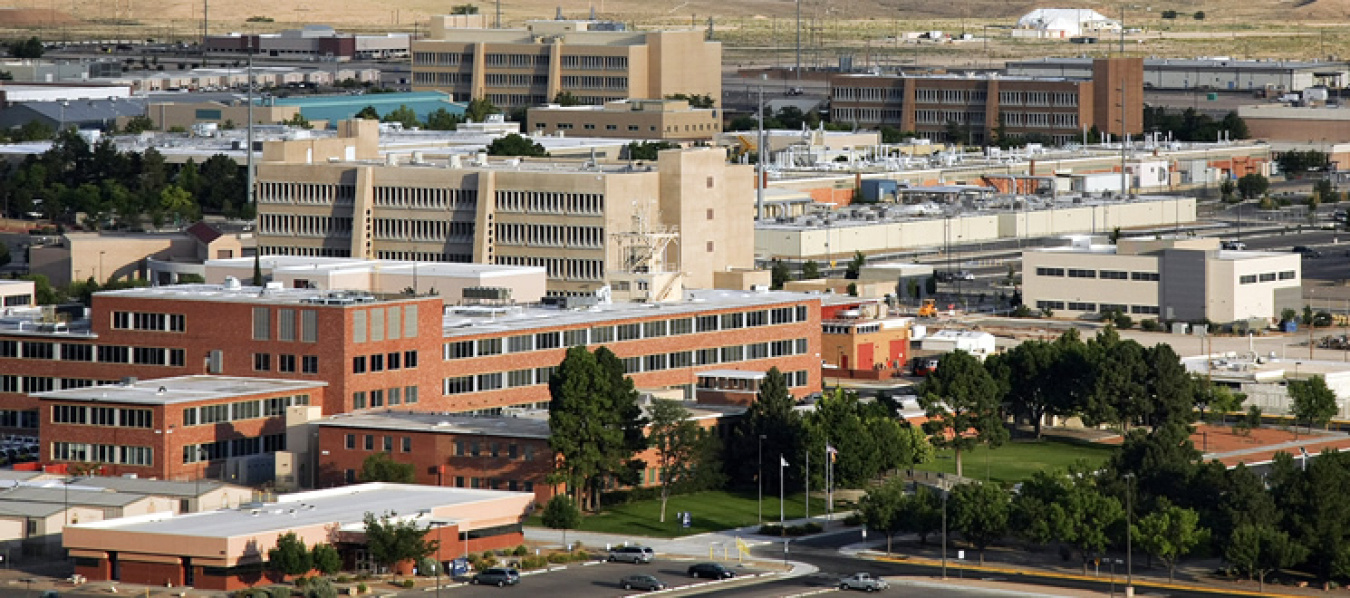
\includegraphics[width=\textwidth]{SandiaNationalLabCoverPhoto2.jpg}
    \end{center}
    \vspace{0.4in}
    % --- UC Davis College of Engineering Logo ---
    \begin{center}
        
\includegraphics[width=3in]{COE.png}
    \end{center}
    \vspace{0.6in}
    % --- Project Title ---
    \begin{center}
        {\LARGE\bfseries\color{blue!70!black} \projecttitle}\\[12pt]
        {\large\bfseries SPONSORED BY: \MakeUppercase{\sponsor, \organization}}
    \end{center}
    \vfill  % Push the following content to the vertical center/bottom

    % --- Report Type ---
    \begin{center}
        {\large\bfseries PRELIMINARY MACHINE ARCHITECTURE REPORT}
    \end{center}

    \vspace{0.4in}

    % --- Course Information ---
    \begin{center}
        {\large \coursename}\\[4pt]
        {\large \MakeUppercase{\instructor}}\\[4pt]
        {\large \MakeUppercase{\ta, Teaching Assistant}}
    \end{center}

    \vspace{0.4in}

    % --- Submission Deadline ---
    \begin{center}
        {\large\bfseries SUBMISSION DEADLINE: \MakeUppercase{\duedate}}
    \end{center}

    \vspace{0.5in}
\end{titlepage}


% ============================================================================
% TEAM MEMBER PAGE
% ============================================================================
% This page lists all team members, as shown in the Report 2 Template.
% The grading rubric (Section I) checks that all names are present.
% ============================================================================

\newpage
\thispagestyle{empty}  % No header/footer on this page either

\vspace*{1in}
\begin{center}
    {\Large\bfseries Team \teamnumber}\\[24pt]

    % --- List all team members ---
    % TODO: Verify spelling of all names
    {\large
        Isaiah Mathew\\[8pt]
        Jon Pizarro\\[8pt]
        Nicholas Metta\\[8pt]
        John Bodine\\[8pt]
        Miguel Cuaycong\\[8pt]
        Sam van der Veen\\[8pt]
    }

    \vspace{0.6in}

    {\Large\itshape \projecttitle}\\[12pt]
    {\large By the}\\[12pt]
    {\Large\bfseries \teamname}\\[24pt]
    {\large Sponsored by \sponsor, \organization}\\[36pt]
    {\large Preliminary Machine Architecture Report}\\[12pt]
    {\large \coursename}\\[6pt]
    {\large \instructor}\\[6pt]
    {\large TA \ta}\\[12pt]
    {\large Due \duedate}
\end{center}


% ============================================================================
% TABLE OF CONTENTS
% ============================================================================
% GRADING: Section 1.3 — 5.0 points
%   "Accurate page numbers, headings and sub-headings used"
%
% LaTeX generates this automatically from \section and \subsection commands.
% You MUST compile TWICE for page numbers to update correctly.
% ============================================================================

\newpage
\tableofcontents
\listoffigures
\listoftables

\newpage  % Start the body of the report on a fresh page

\chapter{Abstract}
\label{sec:abstract}

%--- BEGIN CONTENT ---

Sandia National Laboratories has tasked our senior design team, 
the \teamname, to design a passive temperature compensation device (\device) that regulates gas flow. 
The device must restrict its orifice as the ambient temperature of the surrounding air increases.
The \device\ must be purely thermo-mechanically driven, functioning without reliance on embedded systems (electronics and controls) or user input.
The required mathematical relationship between the ambient temperature and a characteristic orifice geometry, as provided by Sandia National Labs (SNL, a.k.a. the "sponsor"),
stipulates that the orifice maintain an effective diameter that varies with temperature between 200 and 500 $\mu$m, or half the width of the ballpoint on a pen,
with an average tolerance of $\pm 13\ \mu$m, about one fifth the thickness of a human hair.
Our team designed three interconnected subsystems to accomplish this objective:

\begin{itemize}
    \item A square valve orifice, comprising two overlapping square holes
    \item A passive thermal actuator, which expands with rising temperature and drives the valve
    \item A mount, which fixes the relative positions of the other subsystems
\end{itemize}

After presentation of our initial design concepts, SNL awarded our team \$2,000 to purchase, manufacture, assemble, and test the \device.
This Preliminary Machine Architecture Report explains and dimensions each subsystem in detail, outlines our design criteria, and demonstrates requirement satisfaction.

\chapter{System Architecture}
\label{sec:system_architecture}

    \section{System Requirements}
    \label{sec:initial_system_requirements}
        Sandia National Labs provided us with exactly two system requirements, 
        defined precisely as follows:

        \begin{enumerate}
            \item The device must passively restrict the provided flow of gas without external input or control such that the effective diameter of its orifice obeys the following relationship with the ambient temperature of the outside environment:
            
                \begin{equation}
                    \requiredRelationship
                    \label{eq: required_relationship}
                \end{equation}

                Where:
                \begin{align*}
                    &A_1 = \specDeffConstOne \specTolerancePercent\ \frac{\text{mm}}\degC
                    \\
                    &A_0 = \specDeffConstTwo \specTolerancePercent\ \text{mm}
                    \\
                    &T_{\text{reference}} = \specTempRef \degC
                    \\
                    &T_{\text{ambient}}\ \in\ [\specTempLow, \specTempHigh] \degC 
                \end{align*}

            \item The device must remain within a mechanical envelope of 10 cm x 10 cm x 10 cm
        \end{enumerate}
        
        These will be referred to as the “Required Relationship” and the “Mechanical Envelope” throughout the remainder of the report. They are a strict requirement and a soft guideline, respectively.
        A mechanical envelope is the total volume that the device is allowed to occupy at all times.
        When defining specifications that comply with this requirement, the required dimensions will vary for each principal axis.
        Thus, for clarity, the system axes will be defined as follows:

        \newpage

        % NOTE - These are consistent with the main CAD assembly axes
        \begin{itemize}
            \item The "Longitudinal" axis (z-axis) runs upstream along the direction of gas flow
            \item The "Vertical" axis (y-axis) points directly upwards
            \item The "Lateral" axis (x-axis) is perpendicular to each other axis and points right as one looks downstream
        \end{itemize}

        These are depicted in Figure \ref{fig:mainIsometric}.

        Equation \eqref{eq: required_relationship} is characterized by a linear relationship with the following extrema:

        \begin{equation}
            \coldBoundary
            \label{eq: coldBoundary}
        \end{equation}
        
        \begin{equation}
            \hotBoundary
            \label{eq: hotBoundary}
        \end{equation}

        \begin{equation}
            \DTref
            \label{eq: DTref}
        \end{equation}

        These tolerance values are derived in Appendix \ref{app:errorProp}.
        The effective diameter of an orifice of any geometry is the diameter of a circle with equivalent area, such that
        
        \begin{equation}
            A = \frac{\pi}{4}D_{\text{effective}}^2
            \label{eq:d_eff}
        \end{equation}
        
        In order to passively drive the valve orifice diameter by ambient temperature change, 
        our team developed three sub-architectures:
        a valve, to restrict the flow;
        an actuator, to drive the valve movement,
        and a mount, to fix the relative positions of the two.

        In addition to these requirements, our sponsor supplied us with the following design conditions:
        
        \begin{enumerate}
            \item The upstream gas pressure $P$ will lie within the range $0.6895\ \text{MPa} \leq P \leq \specPressure\ \text{MPa}$.
            \item The ambient temperature will vary within the range $-60 \degC \leq T_{\text{ambient}} \leq 80 \degC$.
            \item The provided gas will be up to 20 $\degC$ hotter than the ambient air.
            \item The gas will be a noble gas or Hydrogen.
            \item The gas will be supplied by a stainless steel pipe between 1.524 mm and 25.4 mm in diameter.
            \item The ambient temperature will remain fixed during operation.
            \item The device will be tested by the sponsor to validate required compliance, both without gas flow and for up to 60 seconds with gas flow
        \end{enumerate} 
        
        The \device\ must withstand the extreme pressure, operate within a wide temperature range, 
        and isolate the temperature-sensitive device controller
        from heat transfer from the internal gas for a full minute during operation.
        Hydrogen is apt to diffuse through flexible surfaces; thus, all wetted parts must be compatible with Hydrogen and prevent its diffusion.
        This leaves little room for additional design criteria. Each subsystem must accomplish its mission to extremely small tolerance
        despite these conditions and any errors introduced by every other subsystem.
        
        Thus, to maximize the \device 's potential for success, we proceeded with one chief criterion beyond the necessary specifications:
        the selected architecture should be as simple as possible. Through several iterative changes,
        we developed the following system architecture.

    \section{System Architecture Overview}
    \label{sec:sys_arch_overview}
        
        The \device\ (Figures \ref{fig:mainIsometric}, \ref{fig:mainExploded}, and \ref{fig:SubAssemblyID})
        comprises the following subassemblies:

        \begin{itemize}
            \item Valve: the central orifice, its valve stem, and a hermetically sealed bellows sit in the central housing component.
                    These are welded to the housing inlet and outlet, which will connect to the provided gas flow pipes, to make the complete housing structure.
            \item Actuator: the thermal expansion block sits nested inside the mount superstructure. 
                    It is welded between the upper interior of the mount and the tip of the valve stem.
            \item Mount: the device superstructure is welded and bolted together to hold the actuator from its top at a fixed distance from the valve orifice.
        \end{itemize}
       
       

        \begin{figure}[H]
            \centering
            \begin{tikzpicture}
                \node[anchor=south west, inner sep=0] (image) {
                    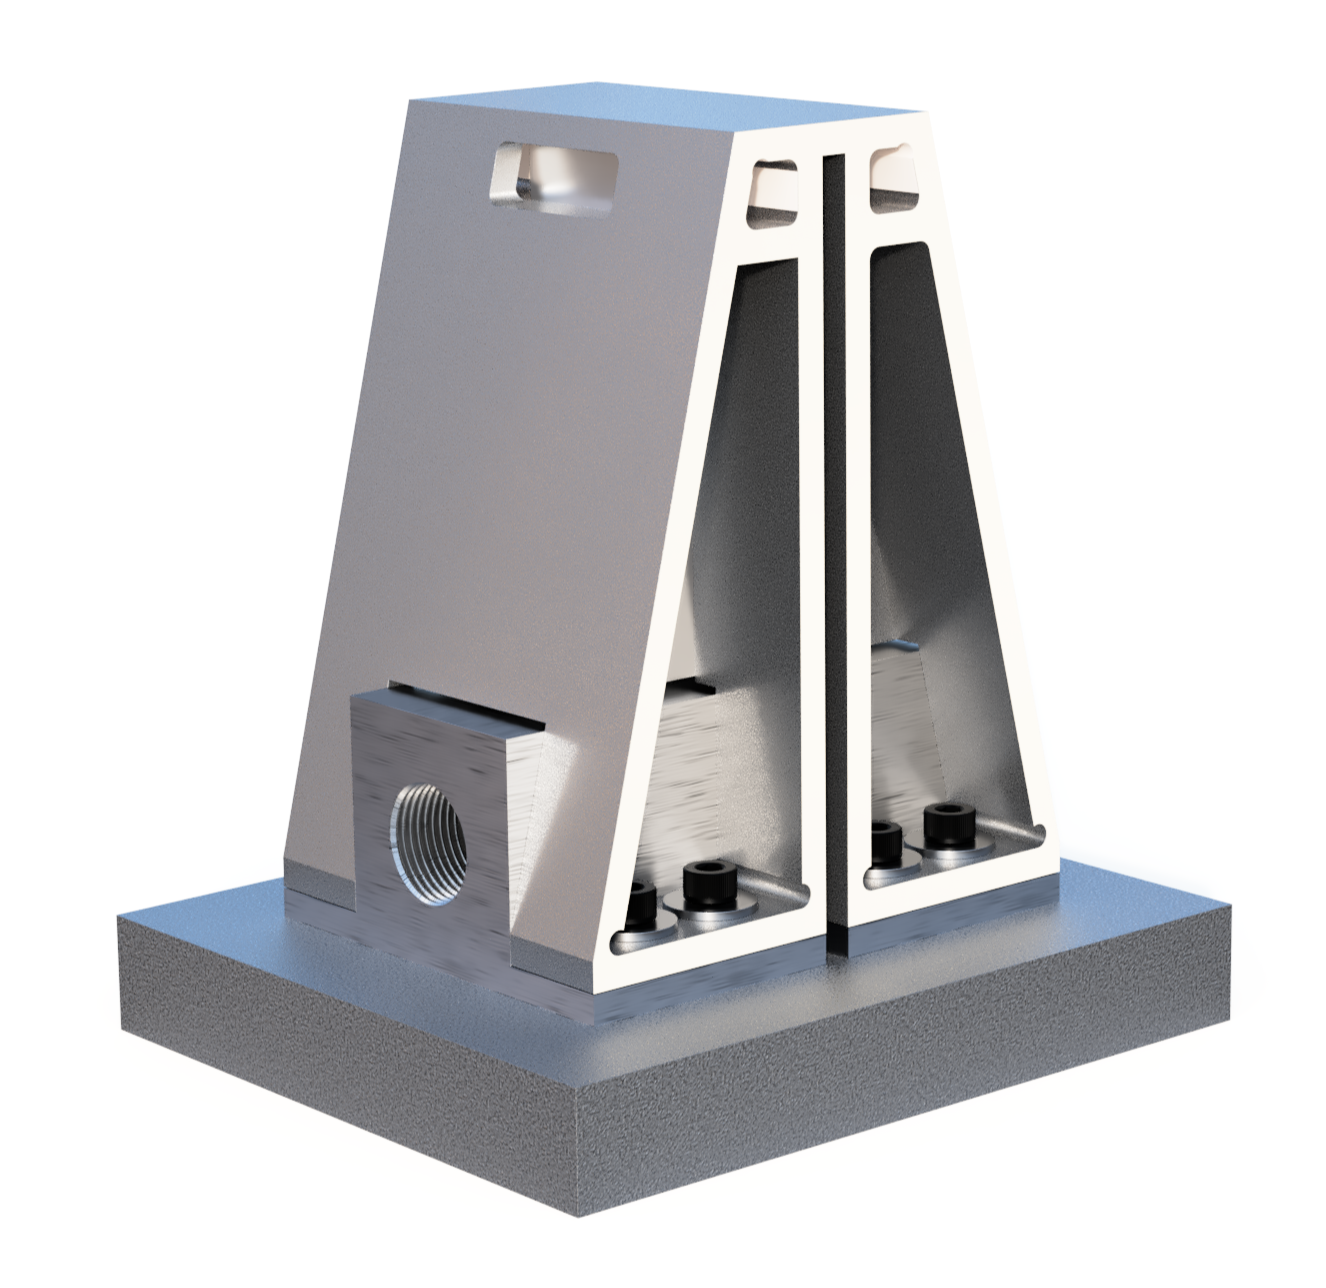
\includegraphics[height=4in, width=6in, keepaspectratio]{Complete_Assembly_Render.png}
                };
                % 3D axes overlay — adjust (0.8, 0.8) to reposition
                \begin{scope}[shift={(1,8)}, thick, >=Stealth]
                    \draw[->] (0,0) -- ({cos(20)},{-sin(20)}) node[right] {$X$};
                    \draw[->] (0,0) -- (0,{1}) node[above] {$Y$};
                    \draw[->] (0,0) -- ({-cos(20)},{-sin(20)}) node[below left] {$Z$};
                \end{scope}
            \end{tikzpicture}
            \caption{Complete assembly}
            \label{fig:mainIsometric}
        \end{figure}

        \begin{figure}[H]
            \centering
            \begin{tikzpicture}
                \node[anchor=south west, inner sep=0] (image) {
                    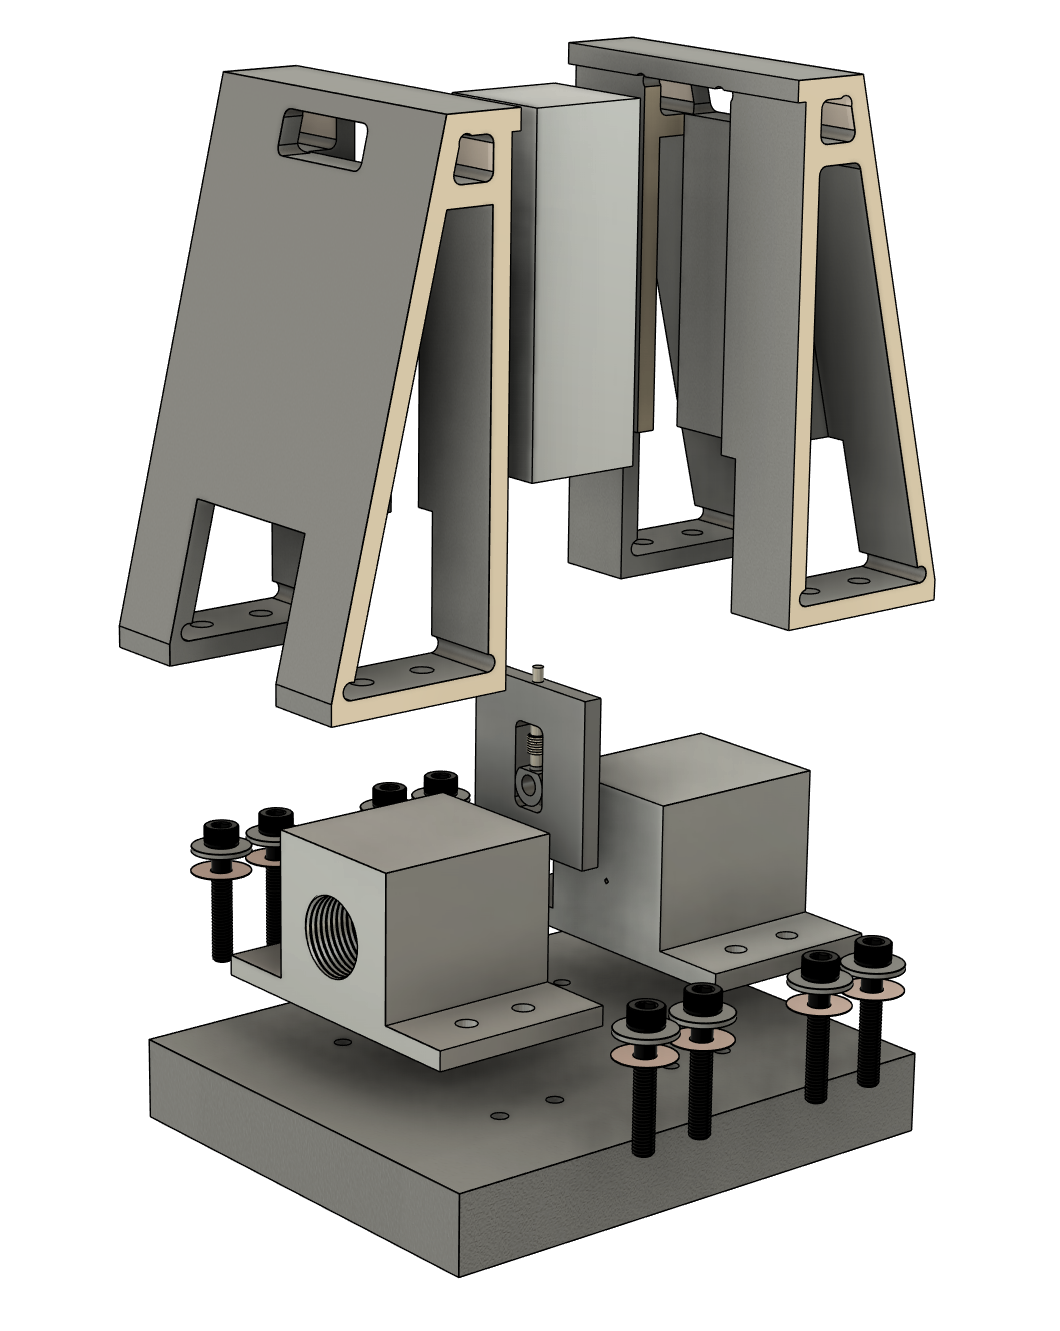
\includegraphics[height=4in, width=6in, keepaspectratio]{CompleteAssemblyExploded.png}
                };
            \end{tikzpicture}
            \caption{Complete assembly exploded view}
            \label{fig:mainExploded}
        \end{figure}

        \begin{figure}[H]
            \centering
            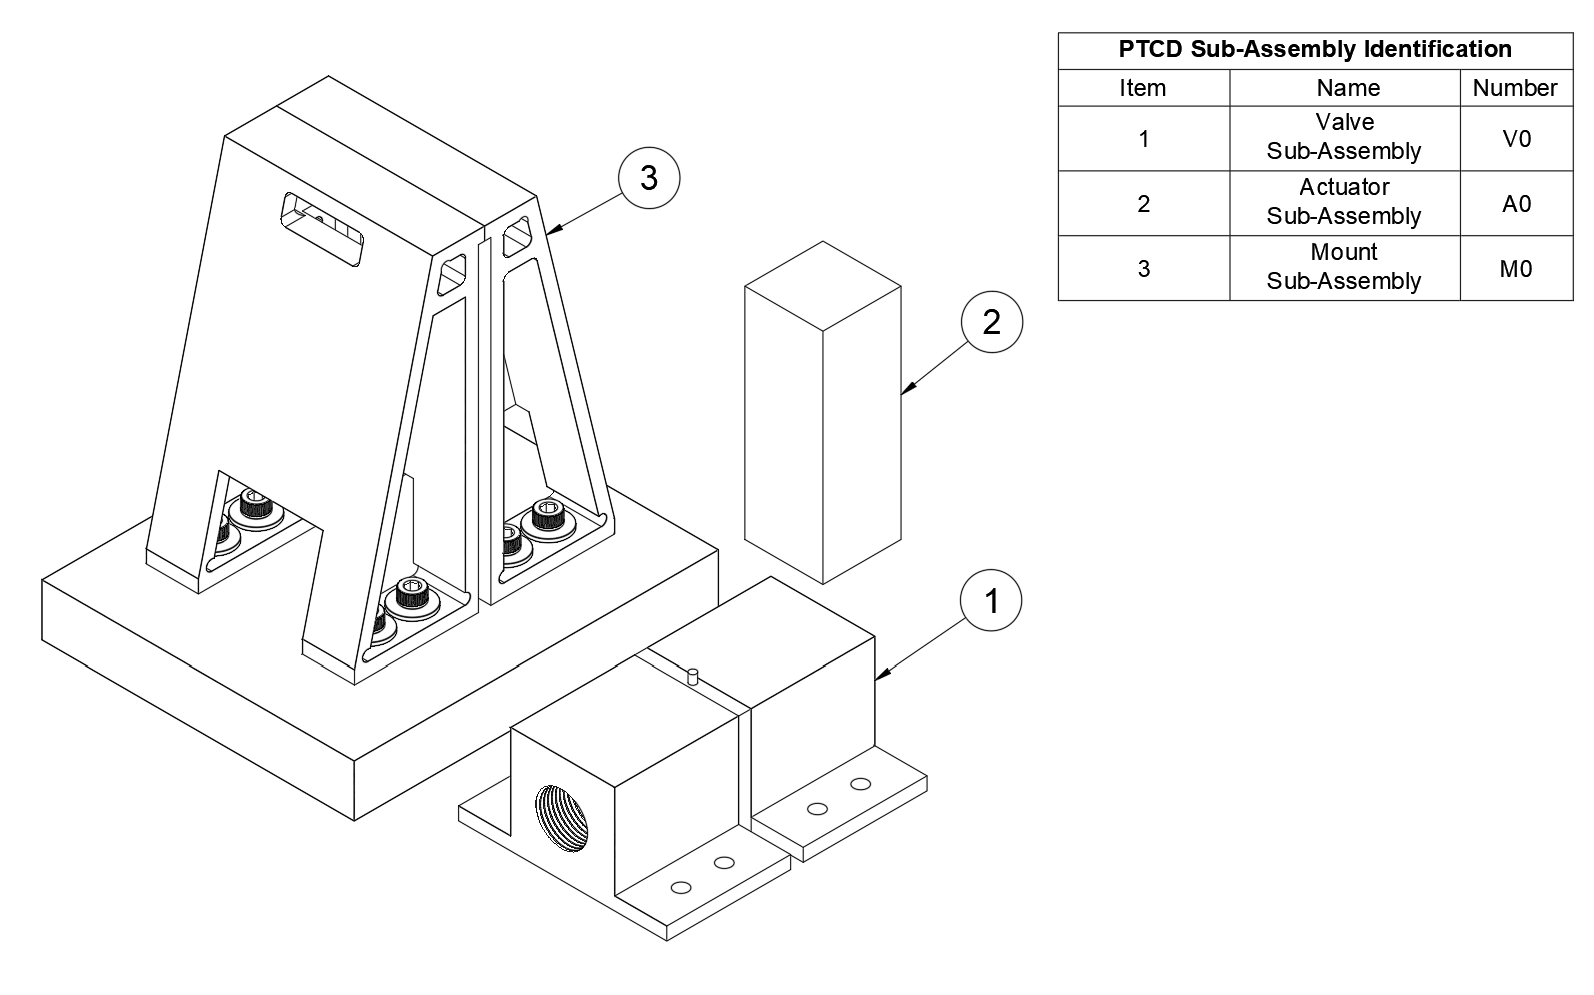
\includegraphics[height=4in, width=6in, keepaspectratio]{SubAssemblyID.png}

            \caption{Sub-assembly identification}
            \label{fig:SubAssemblyID}
        \end{figure}
    
        The valve orifice at the heart of the PTCD comprises two plates with identical square holes cut in them. 
        One plate is fixed to the valve housing; the other is free to move vertically as driven by the valve stem. 
        The two square holes lie flush against one another and are vertically offset such that only a small square opening appears between the valve inlet and its outlet. 
        If the two holes were circles, they would resemble a Venn diagram; thus, as pictured in Figure \ref{fig: orifice}, the overlap between these squares constitutes the valve orifice. 
        The lower (blue) square is cut into the moving plate, referred to as the “central plate” in this report, such that as the valve stem drives the plate downwards, the valve orifice (represented by the gray square) constricts.
        
        A rigid mount suspends the thermal actuator, a block of aluminum, above the assembly. 
        The valve stem is welded to the free base of the actuator such that, as the ambient temperature increases, the actuator base extends downwards, driving the valve stem and central plate downwards with it and closing the valve orifice. 
        As the temperature decreases, the actuator pulls the central plate back up, opening the orifice again. Across the total design temperature range, the actuator expands 267 $\mu$m, driving the valve an equal distance.

        \begin{figure}[H]
            \centering
            
\includegraphics[height=2in]{orifice.png}
            \caption{Orifice geometry}
            \label{fig: orifice}
        \end{figure}

        Thus, the entire system can be summarized by the open-loop control diagram represented by Figure \ref{fig:controls_diagram}, where X is the vertical distance between the two central vertices.
        According to control systems theory\cite{ref_Nise}, a passive device is represented by an open-loop control diagram with no sensor feedback.
        The system transfer function inputs $T_{\text{ambient}}$, outputs $D_{\text{effective}}$, and can be represented by the general equation \ref{eq: transfer_function}:
        
        \begin{equation}
            D = \frac{dD}{dT} \Delta T + D_0
        \end{equation}

        which can be expanded,
        
        \begin{equation}
            \transferFunction
            \label{eq: transfer_function}
        \end{equation}

        This must equal the Required Relationship in equation \ref{eq: required_relationship}. 
        Therefore,

        \begin{equation}
            \frac{dD_{\text{eff}}}{dX} \cdot \frac{dL}{dT}\frac{dX}{dL} = A_1
            \label{eq:actuator_control}
        \end{equation}

        The control derivative $\frac{dL}{dT}$ will be governed by the actuator. 
        $\frac{dX}{dL}$ will be governed by the valve subsystem.

        \begin{equation}
            \frac{dD_{\text{eff}}}{dX} \cdot X(T_{\text{ref}}) = A_0
            \label{eq:mount_control}
        \end{equation}

        The constant $X(T_{\text{ref}})$ is governed by the mount subassembly.
        Finally,

        \begin{equation}
            D_{\text{effective}} = - \sqrt{\frac{2}{\pi}} \cdot X
            \label{eq:D_X}
        \end{equation}

        \begin{equation}
            \frac{dD_{\text{eff}}}{dX} = - \sqrt{\frac{2}{\pi}}
            \label{eq:valve_control}
        \end{equation}

         as calculated in Appendix \ref{app:orifice_geometry}. The control derivative $\frac{dD_{\text{eff}}}{dX}$ is governed by the valve subassembly.


        \begin{figure}[H]
            \centering
            \includegraphics[height=3in]{controls_diagram.png}
            \caption{\device\ open-loop control diagram}
            \label{fig:controls_diagram}
        \end{figure}

        In the context of these governing equations, the following sections define the selection criteria for each subsystem and qualitatively describes the optimal architecture we selected to meet these specifications.
        Subsystem specifications, if properly defined, guarantee that a device whose subsystems keep their requirements will in turn keep the requirements.
        These serve three purposes:

        \begin{enumerate}
            \item To define the component of the system-control transfer function (eq. \ref{eq: transfer_function}) for which that subsystem is responsible
            \item To limit deviation from that transfer function such that the total error remains within the tolerance allowed by eq. \ref{eq: required_relationship}
            \item To limit error that affects the specifications of other subsystems
        \end{enumerate}

        Several specifications serve two other purposes: two limit the mechanical envelope of each respective sub-component
        such that the total mechanical envelope does not exceed the required Mechanical Envelope by more than 35$\%$ 
        (because Requirement 2 was specified as a soft requirement by our sponsor),
        and one prevents catastrophic failure by rupture due to the high-pressure gas.
 


    \section{Valve Subsystem}
    \label{sec:valve_sub_description}

        \subsection{Valve Selection Criteria}
        \label{subsec:valve_sel_crit}

            As detailed in the above section, each subsystem must maintain its portion of the transfer function within enough tolerance such that the whole system satisfies the Required Relationship.
            Tables \ref{tab:valve_specs}, \ref{tab:act_specs}, and \ref{tab:mount_specs} itemize the selection criteria required to keep this relationship for the valve, actuator, and mount subsystems respectively.
            Each table lists the subsystem's core responsibilities on the left, which dictate the behavior of the transfer function or the total mechanical envelope,
            and the individual subsystem specifications necessary to fulfill these responsibilities. The subsequent discussion proves that each subsystem meets the specifications on the right of the table.

            Appendix \ref{app:requirements} lists the full rolldown of requirements to core responsibilities to design specifications.

            \begin{table}[H]
                \centering
                \caption{Valve Selection Criteria}
                \valveSpecs
                \label{tab:valve_specs}
            \end{table}

        \subsection{Valve Architecture}
        \label{subsec:valve_architecture}

            The valve subsystem (Figures \ref{fig:valve_isometric} and \ref{fig:valve_exploded}), colloquially referred to as the "pizza cutter" valve, controls the effective diameter as it is driven by the actuator.
            It consists of the following components, as identified in Figure \ref{fig:valve_id}:

            \begin{itemize}
                \item Housing elements. The housing inlet (V2) and outlet (V3) thread into the pipe providing gas flow.
                         The thread size can be adjusted according to the size of pipe used.
                         These are laser-welded to the housing center (V1), which holds the central valve assembly.
                         Flanges extend from either side of the housing to connect to the mount subassembly via its fasteners.
                \item Central valve assembly. Pictured in more detail in Figure \ref{fig:valve_wireframe}, the valve stem (V4) is welded to the top of the valve orifice (V5). It protrudes through a hole bored in the top of the housing center to connect to the actuator. A bellows (V6) is used to hermetically seal this hole.
            \end{itemize}
            
            \begin{figure}[H]
                \centering
                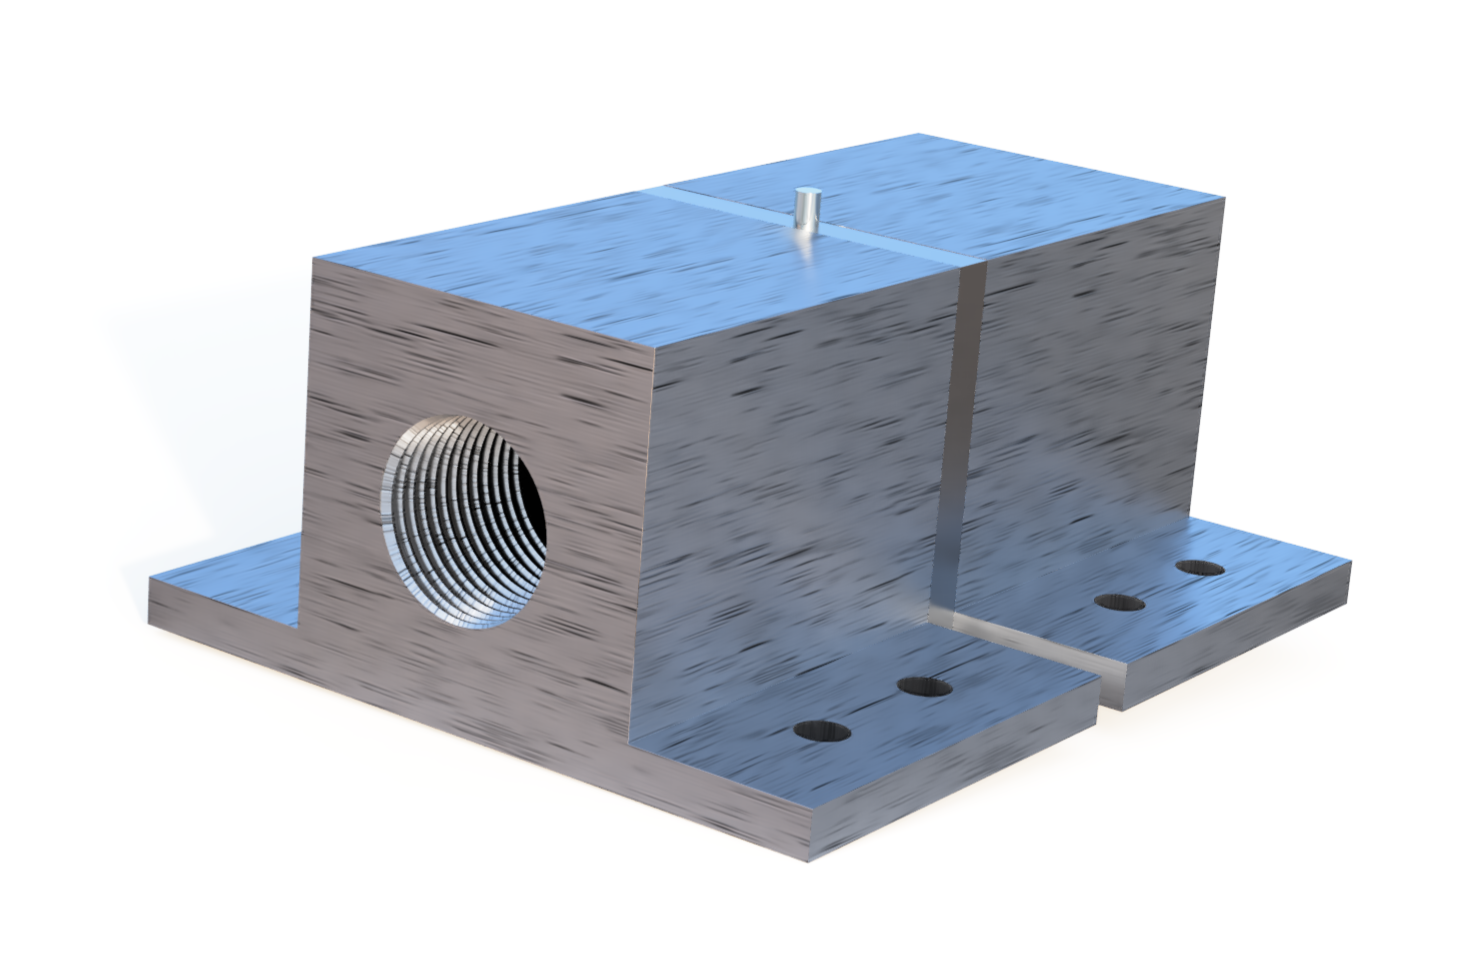
\includegraphics[height=3.5in, width=5.5in, keepaspectratio]{Valve_Subsystem_Render.png}
                \caption{Valve subsystem isometric view}
                \label{fig:valve_isometric}
            \end{figure}

            \begin{figure}[H]
                \centering
                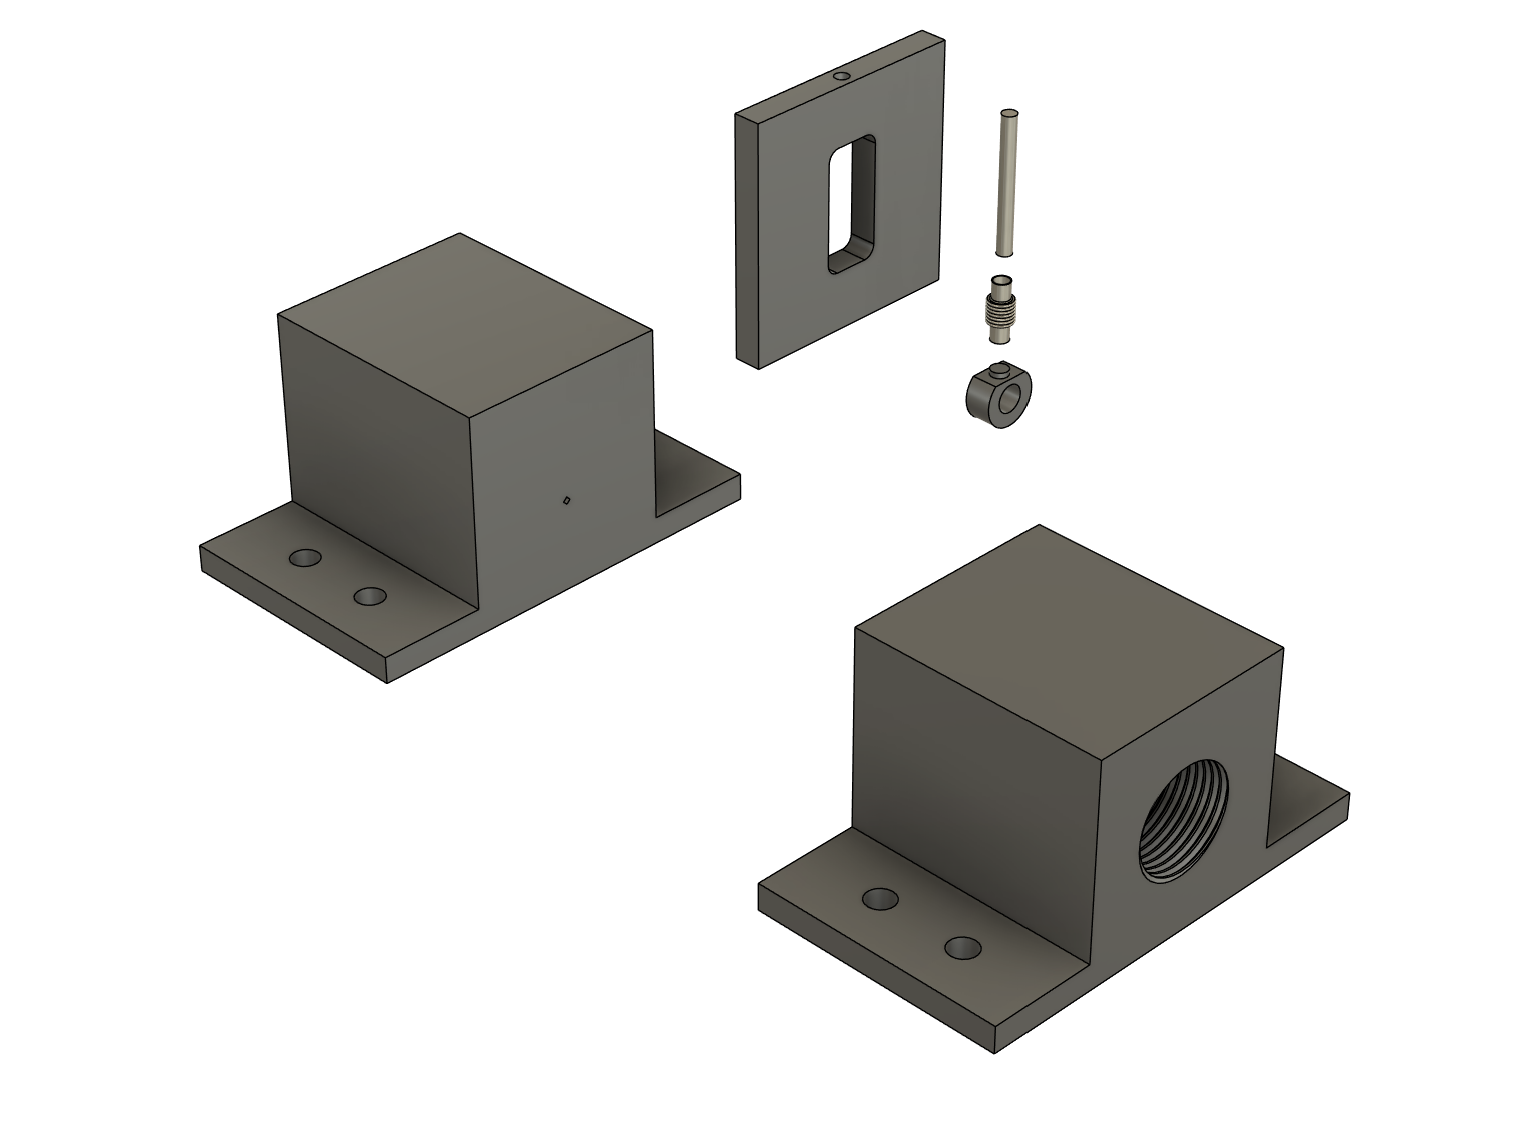
\includegraphics[height=3.5in, width=5.5in, keepaspectratio]{ValveSubsystemExploded.png}
                \caption{Valve subsystem exploded view}
                \label{fig:valve_exploded}
            \end{figure}

            \begin{figure}[H]
                \centering
                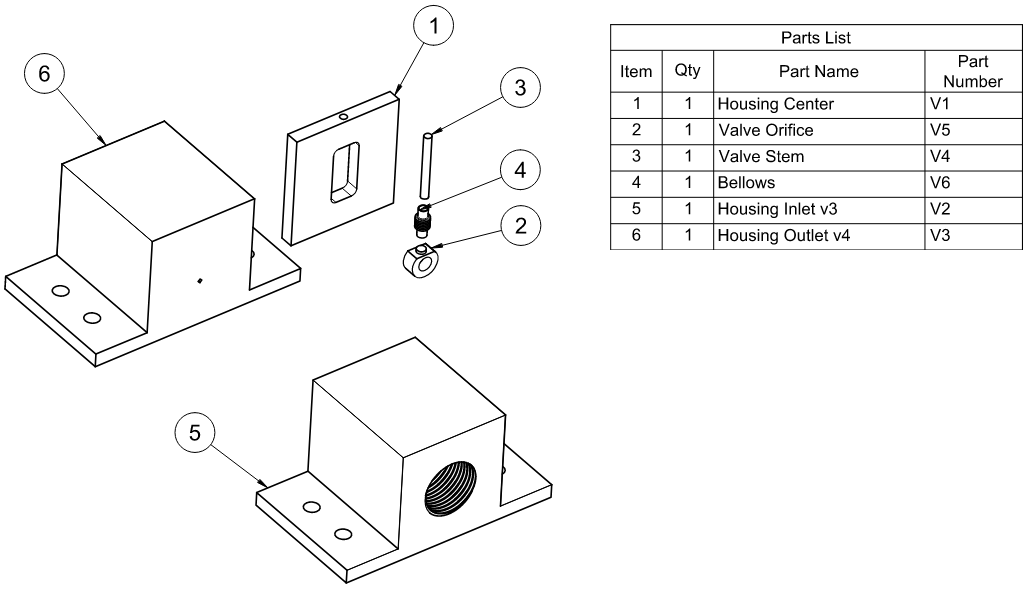
\includegraphics[height=3.5in, width=5.5in, keepaspectratio]{ValveID.png}
                \caption{Valve subsystem with part ID's}
                \label{fig:valve_id}
            \end{figure}

            \begin{figure}[H]
                \centering
                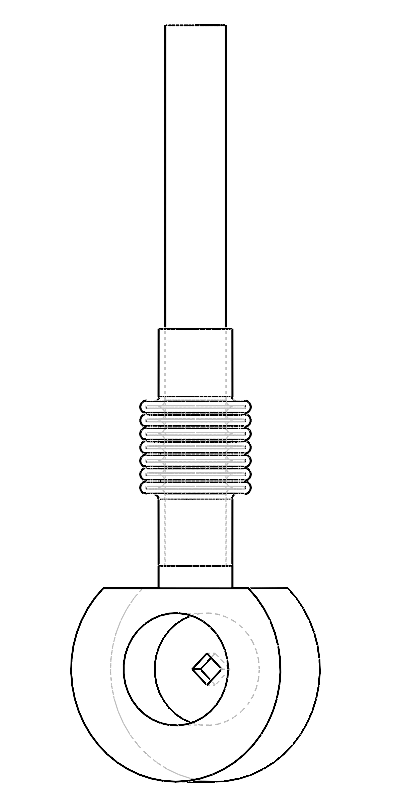
\includegraphics[height=3.5in, width=5.5in, keepaspectratio]{Valve_interior_wireframe.png}
                \caption{Central valve components}
                \label{fig:valve_wireframe}
            \end{figure}

            As pictured in Figure \ref{fig: orifice}, the V5 (referred to as the "valve orifice" and the "central plate" interchangeably) comprises a square diamond cut through its face.
            The housing outlet is similarly cut such that the two holes will slightly overlap.
            The valve stem will drive the central plate downwards, shrinking the orifice. The bellows maintains a hermetic seal, stretching slightly with the valve motion.

            \begin{figure}[H]
                \centering
                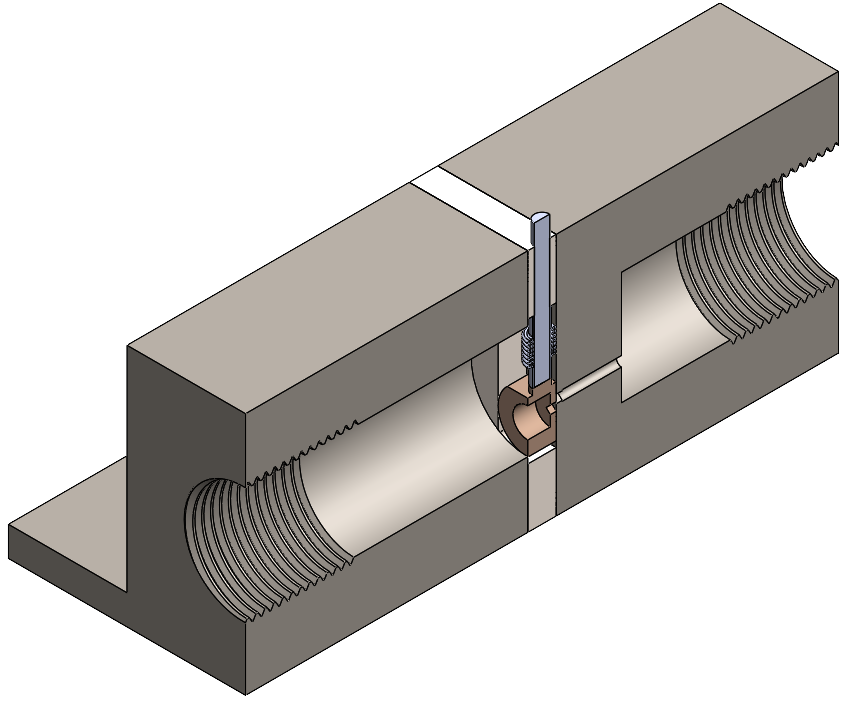
\includegraphics[height=3in, width=5in, keepaspectratio]{Valve_cutaway_isometric.png}
                \caption{Valve subsystem cutaway view}
                \label{fig:valve_cutaway_isometric}
            \end{figure}

            Figures \ref{fig:valve_cutaway_isometric}, \ref{fig:valve_cutaway_normal}, and \ref{fig:valve_cutaway_close} show the internal mechanism once assembled. The central plate sits flush against the housing outlet, held in place by the pressure of the gas flow.
            The resulting orifice, as shown in Figure \ref{fig:valve_interior}, is very small compared to the entire assembly.
            Across the entire temperature range, the maximum orifice size (at the coldest temperature) is about twice the minimum orifice size (at the hottest temperature).

            \begin{figure}[H]
                \centering
                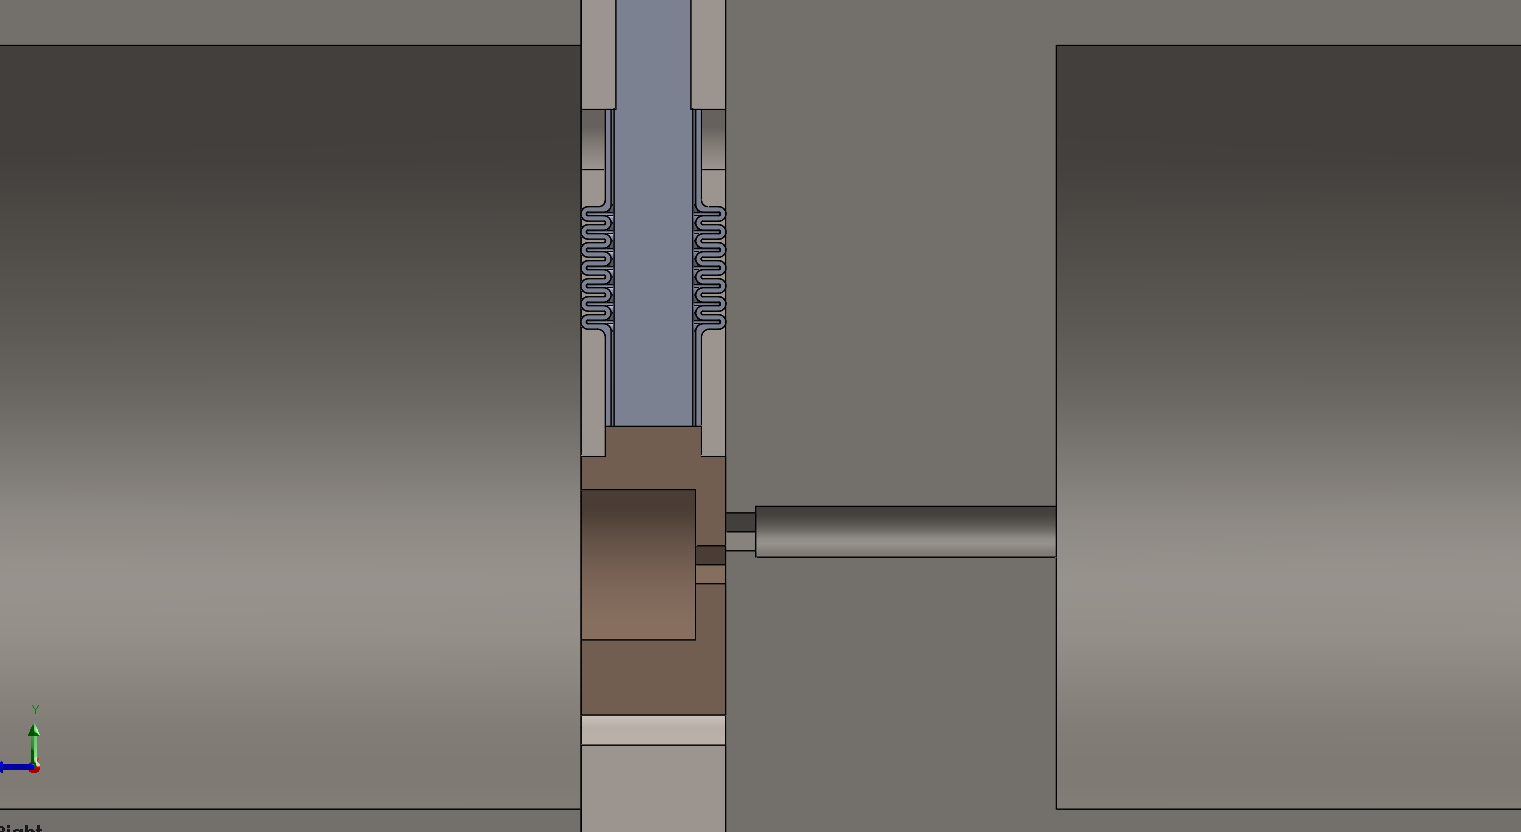
\includegraphics[height=3in, width=5in, keepaspectratio]{Valve_cutaway_normal.png}
                \caption{Valve subsystem internal mechanism}
                \label{fig:valve_cutaway_normal}
            \end{figure}

            \begin{figure}[H]
                \centering
                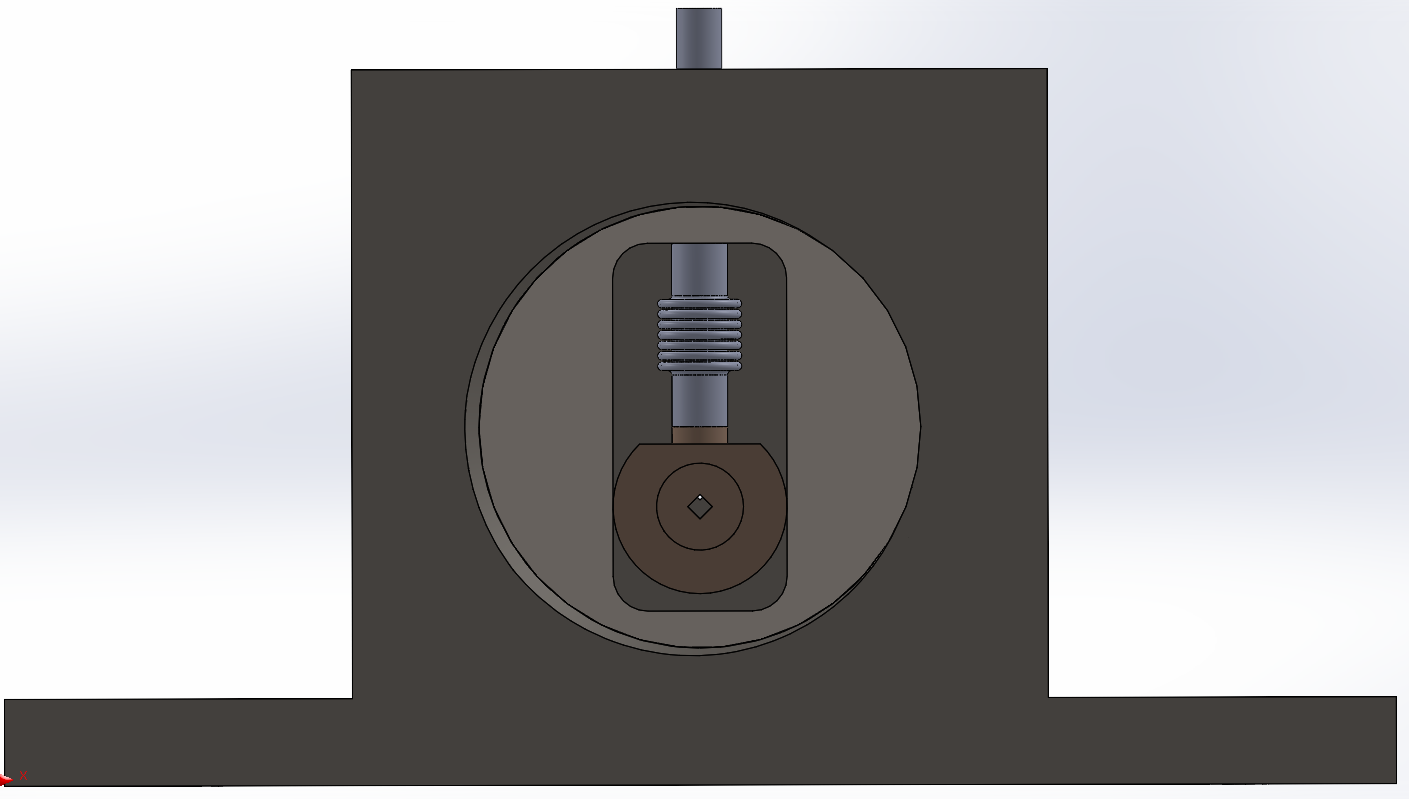
\includegraphics[height=3in, width=5in, keepaspectratio]{Valve_interior.png}
                \caption{Valve orifice front view}
                \label{fig:valve_interior}
            \end{figure}

            \begin{figure}[H]
                \centering
                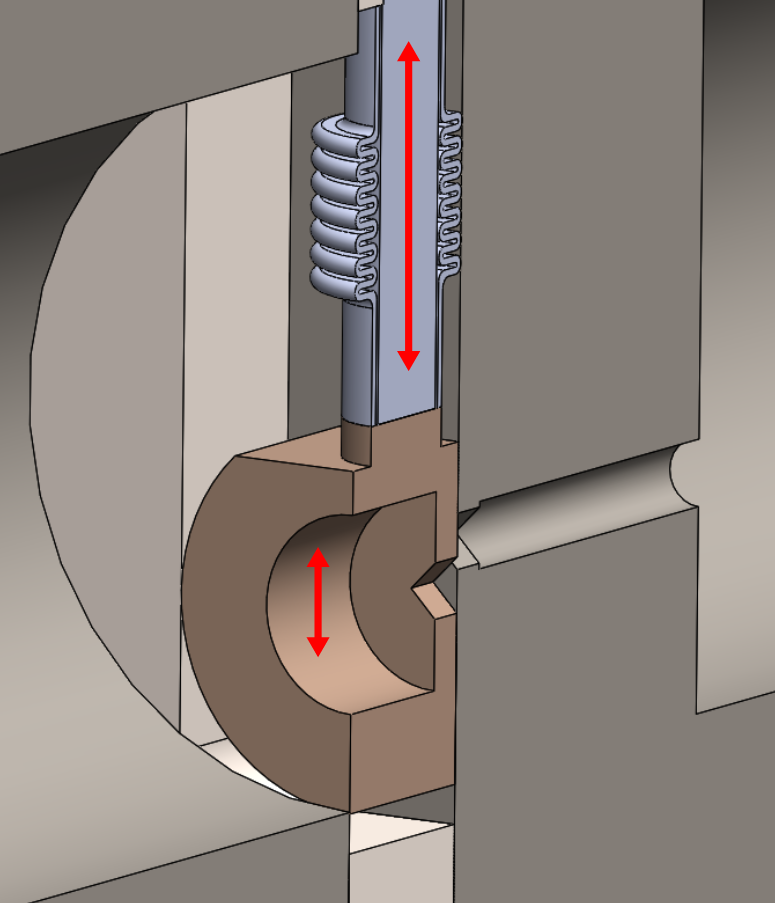
\includegraphics[height=3in, width=5in, keepaspectratio]{Valve_cutaway_close.png}
                \caption{Valve orifice internal mechanism, close view}
                \label{fig:valve_cutaway_close}
            \end{figure}

            Despite the patent difficulty in manufacturing a square hole of this size, our team selected this architecture with two motivations:

            \begin{enumerate}
                \item The required relationship between $T_{\text{amb}}$ and $D_{\text{eff}}$ is linear.
                        If any component delivers a nonlinear output for its input, this will require a complex reparameterization in the other subsystems.
                        Thus, our team selected a system that will maintain a constant value for $\frac{dD}{dX}$.
                        This requires that the orifice overlap maintain a regular polygon shape at all times.
                        Because the square holes are tilted at a $45$ angle, the overlapping hole will also be a tilted square.
                        Its sides will shrink at equal rates, maintaining the square geometry and the desired linear output.
                \item This architecture is simpler than its alternatives. As discussed in Section \ref{subsec:valve_req_updates},
                        other solutions that also promoted the aforementioned linear relationship were deemed too complex, with too many moving components to introduce intolerable error.
                        The "pizza cutter" maintains the desired output while using minimal parts. As shown in the Discussion, this dramatically aids compliance with the subsystem specifications.
            \end{enumerate}


    \section{Actuator Subsystem}
    \label{sec:act_sub_description}

        \subsection{Actuator Selection Criteria}
        \label{subsec:act_sel_crit}

        The actuator subsystem governs the open-loop control derivative $\frac{dL}{dT}$
        as defined in Figure \ref{fig:controls_diagram}, and equations \ref{eq: transfer_function} and \ref{eq:actuator_control}.
        Thus, assuming $\frac{dD}{dX} = -\sqrt{\frac{2}{\pi}}$ and $\frac{dX}{dL} = -1$ within the valve subsystem
        (which is correct practice when calculating error propagation),
        $\frac{dL}{dT}$ must equal $\sqrt{\frac{\pi}{2}} A_1$.
        Because
        $\frac{dL}{dT} = \alpha L_0$,
        two sources drive its error:

        \begin{enumerate}
            \item Changes in the coefficient of thermal expansion (CTE) $\alpha$ across the temperature range
            \item Machining errors in the length of the actuator at $T_{\text{ref}}$, $L_0$
        \end{enumerate}

        Thus, using Kline-McClintock error propagation, the error of $\frac{dL}{dT}$ is calculated as
        
        \begin{equation}
            u_{\frac{dL}{dT}} =
            \sqrt{
                \left( \frac{\partial \left( \frac{dL}{dT} \right)}{\partial \alpha} \cdot u_{alpha} \right)^2 + 
                \left( \frac{\partial \left( \frac{dL}{dT} \right)}{\partial L_0} \cdot u_{L_0} \right)^2}
            \label{eq:udLdX}
        \end{equation}

        where $u_x$ is the error of variable x, and the partial derivatives are evaluated at their variable's respective averages. \cite{ref_Figliola}

        The valve subsystem may also resist the movement of the actuator by providing a reaction force.
        The actuator subsystem must account for any forces it provides within its respective specified limit.

            \begin{table}[H]
                \centering
                \caption{Actuator Selection Criteria}
                \actSpecs
                \label{tab:act_specs}
            \end{table}

        \subsection{Actuator Architecture}


        \begin{figure}[H]
            \centering
            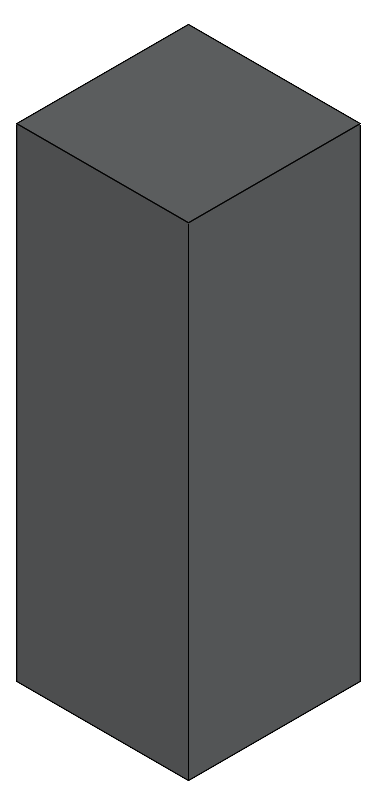
\includegraphics[height=4in, width=6in, keepaspectratio]{Actuator_isometric.png}
            \caption{Actuator block}
            \label{fig:actuator_isometric}
        \end{figure}

            % Paragraph 1
            The actuator subsystem (Figure \ref{fig:actuator_isometric}, part number A0 in Figure \ref{fig:SubAssemblyID}) is a single aluminum block that is driven by ambient temperature changes into a proportional linear displacement. The governing equation of the actuator is $\govActuator$, where $L_0$ is the actuator's free length, $\alpha$ is the coefficient of thermal expansion of aluminum, and $\Delta$T is the difference between 
            the current ambient temperature and determined reference temperature. Since $\alpha$ remains approximately constant throughout the operating temperature range, the relationship between temperature and displacement is linear with minimal error, which will be quantified in Section \ref{subsec:act_spec_1}.

            % Paragraph 2
            The actuator block is mounted between the top inside face of the mount and the top of the valve stem via laser weld. As the ambient temperature rises, the actuator expands downwards pushing the valve stem and translating the plate downward to close the orifice. Similarly, as ambient temperature decreases, the actuator contracts causing the plate to be pulled up, therefore reopening the orifice.
            The actuator is machined to the exact length necessary to expand 267 $\mu$m across the temperature range.

            % Paragraph 3
            One of the most significant design decisions was positioning the actuator block outside the pressure boundary of the valve. It is thermally isolated from the gas flow by the valve housing walls and the bellows assembly. It responds directly to the ambient air temperature instead of the gas temperature.
            This thermal isolation ensures that the 20 $\degC$ difference between the gas and ambient air does not infringe on the operation of the actuator. Moreover, under constraint, the actuator is capable of generating significant thermal stress force that exceeds the friction loads in the system and the bellows spring forces. 
            This force margin ensures reliable actuation across the entire temperature range. 

    \section{Mount Subsystem}
    \label{sec:mount_sub_description}

        \subsection{Mount Selection Criteria}
        \label{subsec:mount_sel_crit}
            The mount subsystem serves as the primary structural interface of the assembly, 
            axially restraining the actuator at one end while transferring reaction forces 
            from the valve subsystem below. 

            The mount must satisfy three primary selection criteria:

            \begin{enumerate}
                \item Sufficient structural rigidity to axially restrain the actuator at its 
                upper boundary condition and withstand the reaction force transmitted upward 
                from the valve subsystem

                \item A low coefficient of thermal expansion $\alpha$ to minimize thermal 
                growth of the mount in the axial direction, ensuring that expansion of the 
                mount does not oppose the intended downward thermal expansion of the actuator

                \item Geometric compatibility with the housing such that the mount 
                structurally integrates all components of the assembly within the required mechanical envelope

            \end{enumerate}

            The second criterion is of particular importance to the function of the device. 
            Because the actuator is designed to expand axially downward into the valve 
            subsystem with increasing temperature, any upward thermal growth of the mount 
            introduces a competing displacement that reduces the net stroke delivered to 
            the valve.


            \begin{table}[H]
                \centering
                \caption{Mount Selection Criteria}
                \mountSpecs
                \label{tab:mount_specs}
            \end{table}

        \subsection{Mount Architecture}
            \begin{figure}[H]
                \centering
                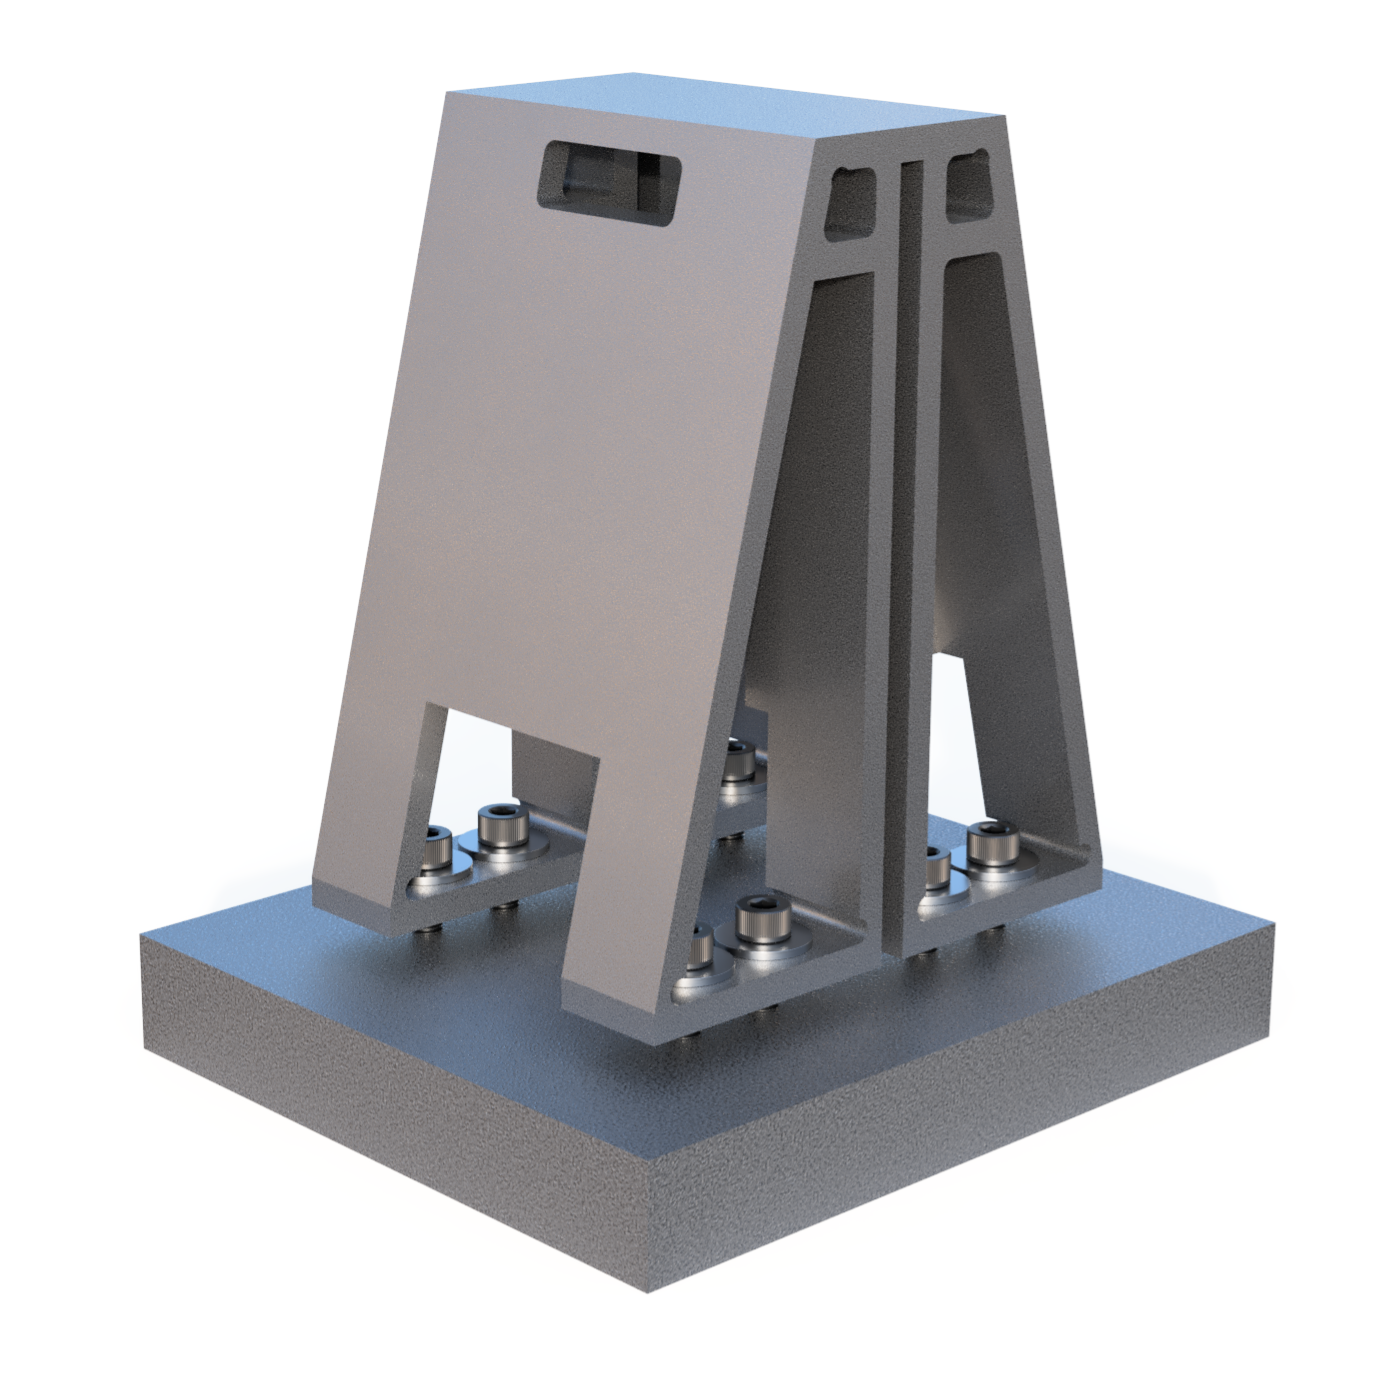
\includegraphics[height=4in, width=6in, keepaspectratio]{Mount_Subsystem_Render.png}
                \caption{Mount subsystem isometric view}
                \label{fig:mount_isometric}
            \end{figure}


            % Paragraph 1
            The mount subsystem (Figures \ref{fig:mount_isometric}, \ref{fig:mount_exploded}) comprises the following components, as identified in Figure \ref{fig:mount_id}:
            \begin{itemize}
                \item Structural components. A fixture (M2) provides a common reference for all the other parts secure to.
                        Two mount parts (M1) sit above the fixture, separated by flanges that extend from the valve housing.
                \item Calibration stack. Eight screws (M3) and washers (M4) mount the valve housing flanges between the mount A-frame and the fixture.
                        To calibrate the height of the mount relative to the housing, eight thick shim washers (M5), thin shim washers (M6), and copper crush washers (M7) are placed between the housing and the mount.
                        The screws are precisely tightened, crushing the washers, until the right tolerance is achieved.
            \end{itemize}

            Note that the screws and washers are all standard metric size M5, not to be confused with their respective part numbers.

            \begin{figure}[H]
                \centering
                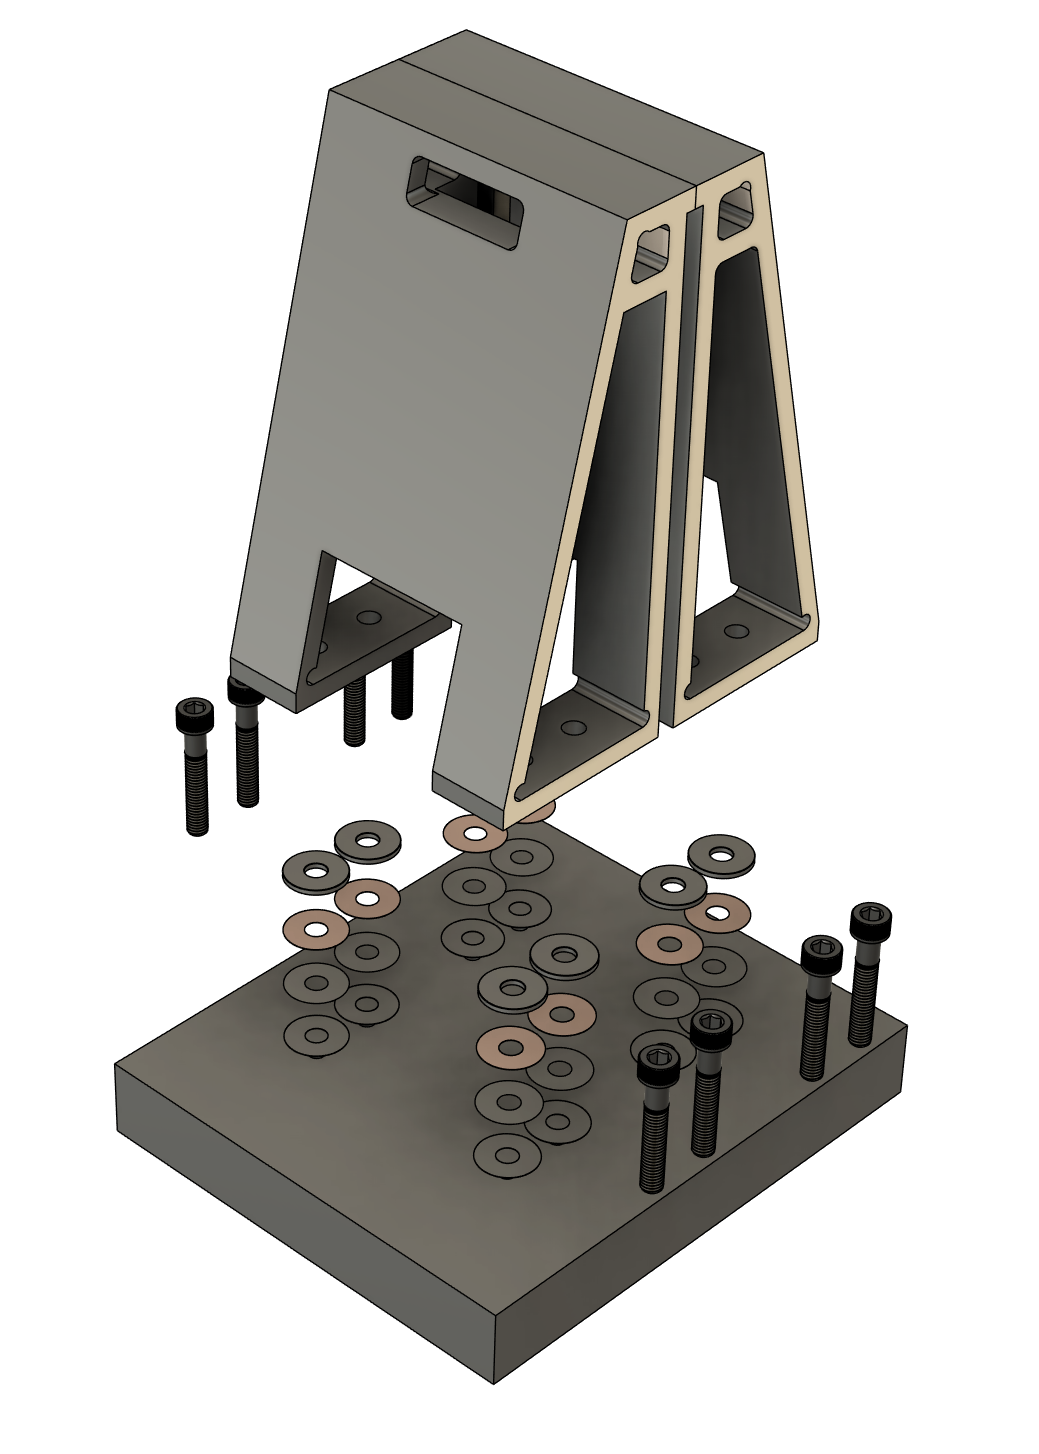
\includegraphics[height=3in, width=5in, keepaspectratio]{MountSubsystemExploded.png}
                \caption{Mount subsystem exploded view}
                \label{fig:mount_exploded}
            \end{figure}

            \begin{figure}[H]
                \centering
                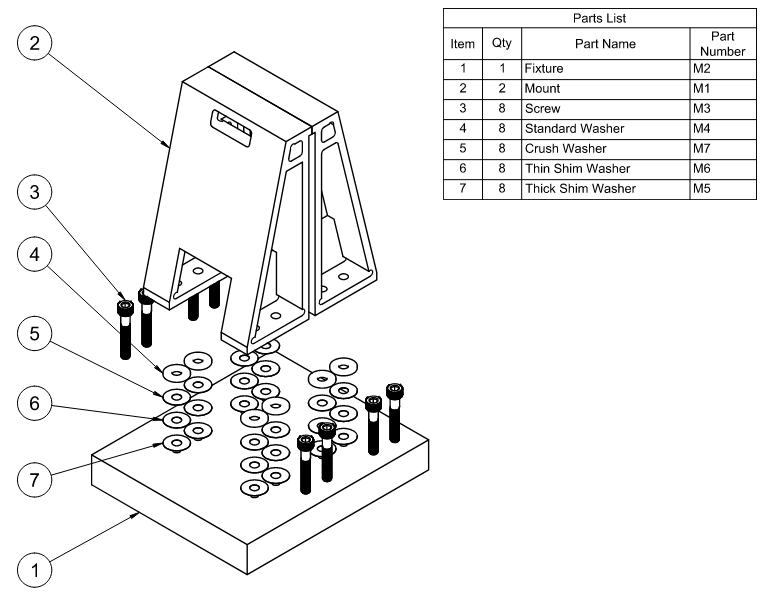
\includegraphics[height=3in, width=5in, keepaspectratio]{MountID.png}
                \caption{Mount subsystem with part ID's}
                \label{fig:mount_id}
            \end{figure}

            % Paragraph 2
            The two trapezoidal mount plates are fabricated from Invar 36 in order minimize the thermal expansion and therefore error caused by the mount. They are vertically oriented to form an A-frame structure and mounted through the housing onto the fixture as seen in Fig. \ref{fig:mount_cutaway_oblique}. The actuator block is housed inside the cavity between the A-frame structure. The upper end is anchored onto the interior top face of the mount.
            The holes machined into the top of each trapezoidal plate provide ease of access for laser welding the top of the actuator to the mount structure. Similarly, the large open windows on the side of the mount plates provide ample clearance for laser welding the valve stem to the actuator at the lowest connection point. These features were designed around the laser beam welding process as each weld joint must be 
            reachable from outside the assembly without having to disassemble adjacent components. The design focus was for the mount geometry to accommodate the welding tool path rather than requiring the weld to be made before the assembly.

            \begin{figure}[H]
                \centering
                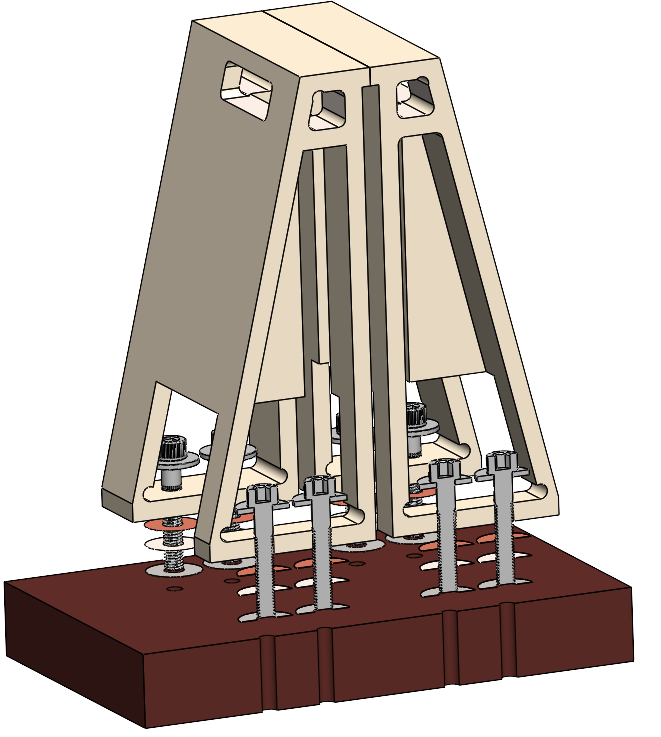
\includegraphics[height=3in, width=5in, keepaspectratio]{Mount_cutaway_oblique.png}
                \caption{Mount subsystem cutaway oblique view}
                \label{fig:mount_cutaway_oblique}
            \end{figure}
            
            % Paragraph 4
            The eight socket head cap screws secure the mount plates to the fixture, which contains corresponding threaded holes and can be assumed to be fixed.
            Each fastener passes through the mount from the top, through the housing, and threads into the fixture at the base. On top of the mount, each screw is seated against a stainless steel washer to distribute the clamping load.
            Between the underside of the mount and the top face of the housing, the three shim washers are stacked in the following order (top to bottom):
            \begin{enumerate}
                \item One annealed copper crush washer
                \item One thin steel shim washer
                \item One thick steel shim washer
            \end{enumerate}
            The crush washer deforms plastically under clamping load to allow for precise positioning during the calibration phase. The thin and thick shim washers provide discrete height adjustment as needed.
            By selecting or combining the shim thicknesses, we can set the precise vertical offset between the mount's actuator anchor point and the valve housing. This shimming capability is the primary calibration mechanism for the PTCD, as the assemble can be shimmed to the correct actuator-to-valve distance during final assembly and testing if any machined dimensions fall outside the desired tolerance.

            % Paragraph 5
            The mount is made of Invar 36, selected for its low coefficient of thermal expansion, machinability, and rigidity.

% ============================================================================
% SECTION 3: DISCUSSION
% ============================================================================
% GRADING: Section IV — 25 points total
%   4.1) Discussion of requirements and rolldown to subsystems (5.0 pts)
%        "Half points well described requirement updates,
%         half points roll down discussion"
%   4.2) Discussion of subsystem interactions (10.0 pts)
%        "Half marks accurate technical discussions, describes how
%         subsystems work together. Half marks for proper engineering
%         drawing package."
%   4.3) Proof that design will meet requirements / calculations (10.0 pts)
%        "Accurate, well motivated / related to requirements,
%         reasonable assumptions stated"
%
% This is the MOST HEAVILY WEIGHTED section (25 pts).
% ============================================================================

\chapter{Discussion}
\label{sec:discussion}
    %--- BEGIN CONTENT ---
    \section{Valve Subsystem}
            As enumerated in Section \ref{subsec:valve_sel_crit}, the Valve Subsystem must meet or exceed the following specifications, listed again in Table \ref{tab:valve_specs_disc}:

        \begin{table}[H]
            \centering
            \caption{Valve Specifications (repeated)}
            \valveSpecs
            \label{tab:valve_specs_disc}
        \end{table}
        \subsection{Specification Compliance}
        \subsubsection{Specification 1: Dimensional tolerances}
        \label{subsec:valve_spec_1}

            As specified, drawings V4 and V5 mandate a tolerance of 1 $\mu m$ on all critical dimensions.

        \subsubsection{Specification 2: Valve Stem displacement}
        \label{subsec:valve_spec_2}


                    The valve will undergo both mechanical compression and thermal expansion due to exposure to temperature change and system forces.
                    Mechanical deformation will occur due to actuation force and is characterized in the following calculation:
                \begin{equation}
                    \delta_{compression} = \frac{F *L_{stem}}{\pi d_{stem}^2/4 E} = 5.0975 \text{ microns}
                    \label{eq:stem_compression}
                \end{equation}


                There will also be minimal thermal expansion from the valve stem itself. The total error from the linear expansion follows the formula:
                \begin{equation}
                    \delta_{thermal} = \alpha_{\text{Invar}} L_{\text{stem}} \Delta T = (1.2 \times 10^{-6})(24.041)(85) = 2.45 \text{ microns}
                    \label{eq:stem_thermal_expansion}
                \end{equation}
                See table \ref{tab:stem_parameters} for the parameter values used in this calculation.

                This is slightly higher than expected but it still much lower than the requirements. In addition, this error is opposite of the compression error caused by the force on the valve stem and by actuator over-expansion (discussed in chapter \ref{sec:act_sub_description}). 
                Note that within the valve stem the total deflection will be that of thermal expansion minus that of compression: $5.0975-2.45 = -2.6475 \text{ microns}$. This magnitude is just lower than the specificaton of 2.75 $\mu$m.

                The valve stem (Figure \ref{fig:stem_bellows_orifice}) transmits mechanical displacement from outside the valve to the orifice plate itself.
                The stem diameter was sized in accordance with the inner diameter of the bellows, and the calculations below validate its structural capability under the surrounding forces present in the assembly.
                The stem must withstand the axial actuation force without yielding or buckling.
                Its material was selected to be Invar 36 for its relatively low coefficient of thermal expansion which thermally insulates the valve from the actuator and prevents thermal expansion of the stem from affecting the valve orifice size.

        \begin{figure}[H]
            \centering
            \includegraphics[height=4in, width=6in, keepaspectratio]{StembellowsOrifice_Render.png}
            \caption{Valve stem, bellows, and orifice plates view}
            \label{fig:stem_bellows_orifice}
        \end{figure}

                \begin{table}[H]
                        \centering
                        \caption{Valve Stem Parameter Values}
                        \label{tab:stem_parameters}
                        \begin{tabularx}{\textwidth}{l X l}
                            \toprule
                            \textbf{Parameter} & \textbf{Description} & \textbf{Value} \\
                            \midrule
                            Material &
                                    &
                            Invar 36
                            \\\addlinespace
                            $d$ &
                            Stem diameter &
                            2.62 mm
                            \\\addlinespace
                            $K_{column}$ &
                            End condition factor &
                            1.0
                            \\\addlinespace
                            $E$ &
                            Young's modulus &
                            148 GPa \cite{matweb}
                            \\\addlinespace
                            $S_y$ &
                            Yield strength &
                            483 MPa \cite{matweb}
                            \\\addlinespace
                            $F$ &
                            Axial actuation force &
                            168.96 N
                            \\\addlinespace
                            $L_{seg}$ &
                            Unsupported length &
                            10.54 mm
                            \\\addlinespace
                            $L_{stem}$ &
                            Total stem length &
                            24.041 mm \cite{matweb}
                            \\\bottomrule
                        \end{tabularx}
                    \end{table}

                Axial stress:
                \begin{equation}
                \sigma_{axial} = \frac{F}{A_{stem}} = \frac{F}{\dfrac{\pi d^2}{4}} = \frac{168.96}{\dfrac{\pi (2.62 \times 10^{-3})^2}{4}} = \frac{168.96}{5.389 \times 10^{-6}} \approx 31.34 \ \text{MPa}
                \label{axial_stress}
                \end{equation}

                The axial stress of $31.34\ \text{MPa}$ is well below the yield strength of $483\ \text{MPa}$, giving a yield safety factor of $S_y / \sigma_{axial} = 483 / 31.34 \approx 15.41$.
                The stem therefore operates comfortably within its elastic range under the full actuation load, and the small diameter is justified by the low force demand.
                \\~\\
                Critical buckling load (Euler):
                \begin{equation}
                P_{cr} = \frac{\pi^2 E I}{(K_{column} L_{seg})^2}, \quad I = \frac{\pi d^4}{64} = \frac{\pi (2.62)^4}{64} \approx 2.313 \ \text{mm}^4
                \label{crit_buck}
                \end{equation}

                \begin{equation}
                P_{cr} = \frac{\pi^2 (148{,}000)(2.313)}{(1.0 \times 10.54)^2} \approx 30{,}413 \ \text{N}
                \label{crit_buck2}    
                \end{equation}

                The stem is laterally guided at the top and bottom, making it a pin-pin column with $K_{column} = 1.0$ and an unsupported length of $L_{seg} = 10.54\ \text{mm}$.
                The critical buckling load yields a buckling safety factor of $30{,}413 / 168.96 \approx 180$.
                Given the short unsupported length of the stem, buckling is not a governing concern for this geometry.
                \\~\\

        \subsubsection{Specification 3: Pressure rating}
        \label{subsec:valve_spec_3}

            The housing consists of three distinct sections: the inlet, the outlet, and the central body, each of which is constructed from 1018 steel and analyzed for its ability to withstand the internal pressure. 
            The housing sections are integrated between the fixture and the mount; they provide the pressure boundary for the valve. The inlet and outlet sections have cylindrical internal geometries with threaded ends that connect to the pipe, while the central body is a rectangular prism that contains the orifice plate and bellows assembly.
            The housing is modeled as a thick-walled cylinder in order to determine the appropriate wall thickness required to sustain the internal pressure.
            The thickness $t$ of the housing is defined as the shortest distance from the inner wall to the outer wall.
            The following equations are used to verify structural integrity under the specified conditions.
            Since internal pressure constitutes the only significant structural load, external forces on the housing are neglected.

            \begin{table}[H]
                            \centering
                            \caption{Valve Housing Parameter Values}
                            \label{tab:housing_parameters}
                            \begin{tabularx}{\textwidth}{l X l}
                                \toprule
                                \textbf{Parameter} & \textbf{Description} & \textbf{Value} \\
                                \midrule
                                Material &
                                &
                                1018 Cold-Rolled Steel
                                \\\addlinespace
                                $r_i$ &
                                Inner radius &
                                9.53 mm
                                \\\addlinespace
                                $t$ &
                                Wall thickness (minimum) &
                                10 mm
                                \\\addlinespace
                                $r_o$ &
                                Outer radius (minimum) &
                                19.53 mm
                                \\\addlinespace
                                $P$ &
                                Internal pressure &
                                \specPressure\ MPa
                                \\\addlinespace
                                $S_y$ &
                                Yield strength &
                                370 MPa \cite{matweb}
                                \\\bottomrule
                            \end{tabularx}
                        \end{table}

            Principal Stresses:
            \begin{equation}
            \sigma_{\theta} = P \left( \frac{r_o^2 + r_i^2}{r_o^2 - r_i^2} \right) = 68.95 \left( \frac{19.53^2 + 9.53^2}{19.53^2 - 9.53^2} \right) \approx 112.05 \ \text{MPa} \quad (\text{Hoop Stress})
            \label{hoop}    
            \end{equation}

            \begin{equation}
            \sigma_{r} = -P \approx -68.95 \ \text{MPa} \quad (\text{Radial Stress})
            \label{radial}  
           \end{equation}

            \begin{equation}
            \sigma_{z} = P \left( \frac{r_i^2}{r_o^2 - r_i^2} \right) = 68.95 \left( \frac{9.53^2}{19.53^2 - 9.53^2} \right) \approx 21.55 \ \text{MPa} \quad (\text{Longitudinal Stress})
            \label{longitudinal}
            \end{equation}
            \\~\\
            Von Mises Equivalent Stress:
            
            \begin{equation}
            \sigma_{vm} = \sqrt{\frac{(\sigma_\theta - \sigma_r)^2 + (\sigma_r - \sigma_z)^2 + (\sigma_z - \sigma_\theta)^2}{2}}
            \label{vonmises}  
            \end{equation}

            \begin{equation}
            \sigma_{vm} = \sqrt{\frac{(112.05 - (-68.95))^2 + (-68.95 - 21.55)^2 + (21.55 - 112.05)^2}{2}} 
            \approx 156.75 \ \text{MPa}
            \label{vonmises2}     
            \end{equation}

            The design is verified if $\sigma_{vm} \leq S_y / FS$; the factor of safety is calculated as follows:
            
            \begin{equation}
            FS = \frac{S_y}{\sigma_{vm}} = \frac{370}{156.75} \approx 2.36
            \label{fs}
            \end{equation}

            The wall thickness of $10\ \text{mm}$ produces a Von Mises stress of $156.75\ \text{MPa}$, yielding a factor of safety of $FS \approx 2.36$.
            The housing design ensures that $10\ \text{mm}$ is the shortest distance from the inner wall to the outer wall therefore the thickness at some points of the housing is greater than $10\ \text{mm}$.
            
            The three sections of the valve housing are joined using welded connections which are designed to withstand the internal pressure without failure.
            Laser Beam Welding (LBW) is used for joint construction with a square butt joint geometry to ensure 
            full penetration \cite{steen2010laser}.
            Full penetration is considered achieved when the weld fuses through the entire wall thickness $t$.
            LBW's high power density enables complete fusion across the interface, and the square butt profile 
            is the optimal geometry for radiographic interpretation, as it ensures defects cannot be obscured 
            \cite{aws2020welding}.
            Weld penetration quality is verified using 100\% X-ray radiographic inspection per ASME B31.3 
            Table 302.3.4 \cite{asme_b313}.
            The circumferential welds are certified to be free of defects such as porosity, lack of fusion, 
            and cracking, all of which could significantly reduce joint strength \cite{aws2020welding}.
            \\~\\
            The viability of the weld joint is evaluated using the ASME B31.3 Pressure Piping Code 
            (Equation 3a or Equation \eqref{tmin_weld}, below) \cite{asme_b313}, which governs the required minimum wall thickness as a function 
            of the weld joint quality factor $E$:
            
            \begin{equation}
            t_{min} = \frac{P D_o}{2(SEW + PY)}
            \label{tmin_weld}
            \end{equation}

            \begin{table}[H]
                \centering
                \caption{Weld Analysis Parameter Values}
                \label{tab:weld_parameters}
                \begin{tabularx}{\textwidth}{l X l}
                    \toprule
                    \textbf{Parameter} & \textbf{Description} & \textbf{Value} \\
                    \midrule
                    $P$ &
                    Internal pressure &
                    \specPressure\ MPa
                    \\\addlinespace
                    $D_o$ &
                    Outer diameter &
                    39.06 mm
                    \\\addlinespace
                    $S$ &
                    ASME allowable stress, $S_y$ / 1.5 &
                    246.7 MPa
                    \\\addlinespace
                    $W$ &
                    Weld strength reduction factor &
                    1.0
                    \\\addlinespace
                    $Y$ &
                    Coefficient for austenitic steels &
                    0.4
                    \\\addlinespace
                    $E$ &
                    Weld joint quality factor &
                    1.0
                    \\\bottomrule
                \end{tabularx}
            \end{table}

            The ASME allowable stress is derived directly from the housing yield strength using the standard 
            code factor of $S = S_y / 1.5 = 370 / 1.5 = 246.7\ \text{MPa}$.
            Per ASME B31.3 Table 302.3.4 \cite{asme_b313}, the weld joint quality factor $E$ depends entirely 
            on the level of examination applied:

            \begin{itemize}
                \item $E = 0.80$: Single butt weld with visual inspection only.
                \item $E = 0.85$: Double butt weld or spot radiography.
                \item $E = 1.00$: Full radiography (100\% X-ray) of all butt welds.
            \end{itemize}

            With full radiography ($E = 1.00$), the minimum required wall thickness is:
            
            \begin{equation}
            t_{min} = \frac{68.95 \times 39.06}{2\left(246.7 \times 1.00 \times 1.0 + 68.95 \times 0.4\right)} 
             \approx 5.17 \ \text{mm}
            \label{t_num}
            \end{equation}

            Since $t_{min} = 5.17\ \text{mm} < t_{actual} = 10\ \text{mm}$, the design is verified.
            The thickness safety factor at the weld joint is:
            
            \begin{equation}
            SF_{weld} = \frac{t_{actual}}{t_{min}} = \frac{10}{5.17} \approx 1.93
            \label{sf_weld}    
            \end{equation}
            \\~\\
            As a secondary check, the peak hoop stress at the inner wall from the thick-wall analysis 
            ($\sigma_\theta = 112.05\ \text{MPa}$) is compared directly against the weld joint allowable stress 
            \cite{asme_b313}:
            
            \begin{equation}
            \sigma_{allow} = S \cdot E \cdot W = 246.7 \times 1.00 \times 1.0 = 246.7 \ \text{MPa}
            \label{stress_allow}
            \end{equation}

            \begin{equation}
            \sigma_\theta = 112.05 \ \text{MPa} < \sigma_{allow} = 246.7 \ \text{MPa}
            \label{ineq_hoop}
            \end{equation}

            The weld joint stress safety factor is:
            \begin{equation}
            SF_{stress} = \frac{\sigma_{allow}}{\sigma_\theta} = \frac{246.7}{112.05} \approx 2.20
            \label{sf_stress}    
            \end{equation}
            
            These results confirm that with 100\% X-ray radiographic inspection ($E = 1.00$) \cite{asme_b313}, 
            the weld joint introduces no strength penalty relative to the base material.
            The joint is viable with a thickness margin of $ 4.83\ \text{mm}$ and a stress safety factor of $2.20$.            
        
        \subsubsection{Specification 4: Temperature gradient}
        \label{subsec:valve_spec_4}

            Formal heat transfer analysis will require extensive computation, which our team will perform during the Spring quarter.
            However, the design is optimized to isolate the actuator from heat transfer from the hotter gas for two reasons:

            \begin{itemize}
                \item The only conductive contact is through the Invar valve stem, which makes minimal surface contact with the actuator.
                \item The entire actuator is exposed to convection with the air or conduction with the mount, both of which are at ambient air temperature and will likely outweigh any heat transfer from the valve stem.
            \end{itemize}

        \subsubsection{Specification 5: Reaction force}
        \label{subsec:valve_spec_5}

            \begin{figure}[H]
                \centering
                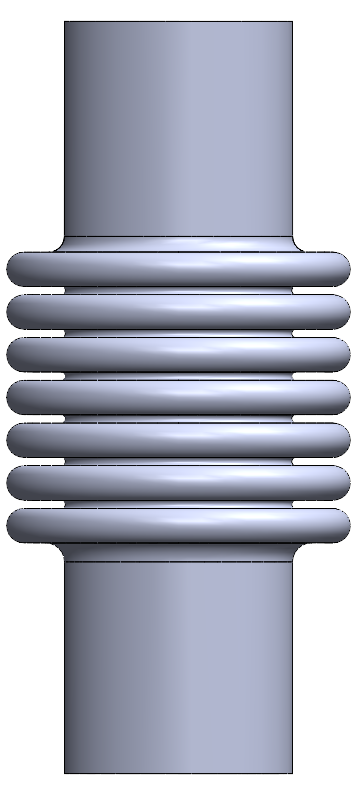
\includegraphics[height=4in, width=6in, keepaspectratio]{bellows.png}
                \caption{CAD model of the bellows}
                \label{fig:bellows}
            \end{figure}

            The welded metal bellows transmits an axial stroke $\delta$ from an external actuator into a high-pressure hydrogen valve while maintaining zero leakage. The bellows must withstand internal pressure $P$, provide the required displacement without plastic deformation, and minimize actuator force demand.
            \\~\\
            Figure \ref{fig:bellows}, illustrates the valve assembly with the bellows. It is laser beam welded to the central valve housing and the valve stem, ensuring a leak-tight seal while permitting the necessary axial movement. 
            This weld joint is one of the first steps
            The following equations address the key design parameters and constraints governing the selection of appropriate bellows geometry and material.
            Accounting for the spring force of the bellows is important for actuator sizing.
            
            Let $K$ be the spring rate of the bellows, which depends on material properties, geometry, and convolution count $N$.
            The spring force is proportional to deflection $\delta$.
            \\~\\

            \begin{table}[H]
                \centering
                \caption{Bellows Parameters}
                \label{tab:bellows_parameters}
                \begin{tabularx}{\textwidth}{l X l}
                    \toprule
                    \textbf{Parameter} & \textbf{Description} & \textbf{Value} \\
                    \midrule
                    Material &
                    Hydrogen Compatible &
                    Inconel 718
                        \\\addlinespace
                    $D_o$ &
                    Outside convolution diameter &
                    4.826 mm
                    \\\addlinespace
                    $D_i$ &
                    Inside convolution diameter &
                    2.616 mm
                    \\\addlinespace
                    $t$ &
                    Wall thickness &
                    0.183 mm
                    \\\addlinespace
                    $L$ &
                    Convolution free length &
                    4.191 mm
                    \\\addlinespace
                    $A$ &
                    Effective area &
                    $10.84 \ \text{mm}^2$
                        \\\addlinespace
                    $N$ &
                    Number of convolutions &
                    7
                    \\\addlinespace
                    $P_{burst}$ &
                    Burst pressure &
                    86.87 MPa
                    \\\addlinespace
                    $k$ &
                    Spring rate &
                    630.46 N/mm
                    \\\bottomrule
                \end{tabularx}
            \end{table}

            Spring force:
            \begin{equation}
            F_s = K \delta = (630.46 \ \text{N/mm})(0.267 \ \text{mm}) \approx 168.96 \ \text{N}
            \label{force_spring}    
            \end{equation}

            The resulting spring force confirms that the stroke demand is well within the elastic operating 
            range of the selected bellows \cite{miniflex_design}.
            The relatively high spring rate of $K = 630.46\ \text{N/mm}$ provides strong squirm resistance 
            under pressure while still producing a manageable spring load given the small stroke $\delta$.
            This balance between stiffness and stroke compliance is central to the optimized selection.
            \\~\\
            Total force required for actuation:
            \begin{equation}
            F_{total} = K \delta + F_{friction} \pm mg \approx 168.96 + F_{friction} \pm mg \ \text{N}
            \label{force_total}
            \end{equation}

            Since $\delta$ is very small, the spring force contribution is modest but nonetheless significant. 
            The term $F_{friction}$ accounts for any additional forces due to friction in the system, which 
            is minimized through careful design and material selection.
            The term $mg$ accounts for gravitational forces acting on the valve stem, which are minimal given 
            the small mass of the stem.
            Together, these contributions result in a low total actuation force demand that is easily 
            achievable with a compact actuator.
            \\~\\
            Critical squirm pressure is the pressure at which the bellows becomes unstable and experiences 
            lateral deformation \cite{miniflex_design}.
            This occurs when the bellows is unrestrained from sideways movement and the internal pressure 
            exceeds the bellows' ability to maintain its shape.
            As noted in the Mini-Flex design guide, squirm will not occur if the bellows is guided internally 
            or externally by a dowel pin, that being the valve stem, or used in a close-fitting bore \cite{miniflex_design}.
            Because the valve body provides lateral restraint, the bellows will not experience squirm, and 
            the critical squirm pressure is therefore not a limiting factor in this design.
            \\~\\
            Burst pressure is the maximum pressure the bellows can withstand while laterally restrained.
            The Mini-Flex design guide defines burst pressure as the minimum internal pressure that will not 
            result in fracture when the bellows is restrained from squirm or sideways movement \cite{miniflex_design}.
            The design is governed by the following relationship:

            \begin{equation}
            P_{operating} < P_{burst} \quad \Rightarrow \quad 68.95 \ \text{MPa} < 86.87 \ \text{MPa}
            \label{ineq_burst}
            \end{equation}

            For this application, the bellows carries a safety factor of 1.26 against burst.
            An optimized design targets a burst safety factor in this range, as too low a factor risks failure 
            under overpressure events, while too high a factor necessitates a larger, stiffer bellows that 
            increases spring load and actuator demand.

        \subsubsection{Specification 6: Mechanical envelope}
        \label{subsec:valve_spec_6}

            As shown in Appendix \ref{app:drawings}, the valve subsystem's maximum mechanical envelope is 
            \begin{itemize}
                \item Longitudinal: 100 mm. This is the sum of the length of the housing inlet and outlet (47.6 mm each) and the housing center (4.8 mm).
                \item Lateral: 80 mm, the width of the housing flanges.
                \item Vertical: 5 mm. Only the thickness of the housing flanges affects the mechanical envelope.
            \end{itemize}
        
        \subsection{Design Requirement Updates}
        \label{subsec:valve_req_updates}

                The core system-level requirements established in the Preliminary Design Report remained 
                unchanged entering the detailed design phase: the valve must produce a linear change in 
                effective diameter with respect to ambient temperature, and must withstand an internal 
                operating pressure of \specPressure\ MPa. What changed substantially was the team's understanding 
                of what could be physically realized given the scale of the device, the number of moving 
                parts, and the tolerancing demands of precision machining at sub-millimeter orifice sizes.

                The Preliminary Design Report selected the hexagonal diaphragm as the valve architecture 
                on the strength of its theoretical properties. The hexagonal geometry was shown analytically 
                to produce a linear relationship between actuator displacement and effective orifice diameter, 
                and it performed well in the screening and scoring matrices on criteria such as force 
                resistance and flow stability. However, as the team moved from concept into detailed design, 
                it became clear that the hexagonal diaphragm presented fundamental manufacturability 
                challenges that could not be resolved within the scope of this project. The design required 
                six independent trapezoidal sliding plates, each interfacing with adjacent plates along 
                precision-machined edges, all operating at an orifice scale thinner than the tip of a 
                ballpoint pen. The tolerance stack-up across six moving parts at this scale introduced 
                unquantifiable uncertainty in the effective diameter, and no feasible assembly sequence 
                could be identified that would allow the device to be built, sealed against \specPressure\ MPa 
                internal pressure, and calibrated reliably. The design was theoretically sound but 
                physically unrealizable under the project constraints.

                Following sponsor feedback and internal reassessment, the team reset its design assumptions 
                and returned to the valve selection problem with manufacturability elevated to a primary 
                constraint alongside linearity and pressure resistance. This shift in perspective produced 
                a fundamentally different solution: a two-plate sliding valve consisting of one fixed plate 
                and one moving plate. The orifice is formed by the overlap between an opening in the fixed 
                plate and an opening in the moving plate. As the actuator displaces the moving plate, the 
                overlapping area changes, producing a linear change in effective orifice diameter. The 
                geometry satisfies the same linearity requirement as the hexagonal design but with a 
                fraction of the part count and a straightforward machining and assembly path.

                This simplification did not eliminate design complexity; it redirected it. By reducing 
                the valve to two plates, the team was able to clearly identify and quantify three new 
                subsystem-level design requirements that the hexagonal design had obscured: managing hoop 
                stress in the valve housing under internal pressure, sealing the valve stem that drives the 
                moving plate through the housing wall, and ensuring the structural integrity of all 
                construction welds. These requirements are tractable and calculable in a way that the 
                tolerance uncertainties of the hexagonal design were not, and they form the basis of the 
                detailed analyses presented in the following sections.

                The transition to the two-plate valve architecture allowed system-level specifications to 
                be rolled down into clearly defined subsystem requirements for the first time. The 
                operating pressure requirement of \specPressure\ MPa rolled down into a housing wall thickness 
                specification governed by thick-wall hoop stress analysis, a weld joint quality requirement 
                mandating radiographic inspection, and a stem seal 
                specification requiring a bellows assembly capable of withstanding full internal pressure 
                without leakage. The linearity requirement rolled down into a geometric constraint on the 
                orifice plate overlap profile, which must be designed such that lateral displacement of 
                the moving plate produces a proportional change in effective diameter across the full 
                temperature operating range. The hydrogen 
                compatibility requirement rolled down into the material specification of Inconel 718 (bellows material) and 1018 steel (housing material) for 
                all wetted components, driven by the need for hydrogen embrittlement resistance, 
                low-temperature toughness, and weld compatibility between the valve stem and bellows 
                assembly.
        
    \section{Actuator Subsystem}
        The Actuator Subsystem must meet or exceed the specifications enumerated in Section \ref{subsec:act_sel_crit}, listed again in Table \ref{tab:act_specs_disc}:

        \begin{table}[H]
            \centering
            \caption{Actuator Specifications (repeated)}
            \actSpecs
            \label{tab:act_specs_disc}
        \end{table}


        \begin{table}[H]
            \centering
            \caption{Actuator Parameter Values}
            \label{tab:actuator_parameters}
            \begin{tabularx}{\textwidth}{l X l}
                \toprule
                \textbf{Parameter} & \textbf{Description} & \textbf{Value} \\
                \midrule
                $E$ &
                Young's modulus &
                $\specYoungMActuator$
                \\\addlinespace
                $A$ &
                Cross-sectional area &
                $\specCrossSectArea$
                \\\addlinespace
                $\alpha$ &
                Coefficient of thermal expansion &
               $ \specActuatorCTE$
                \\\addlinespace
                $L_0$ &
                Original actuator length &
                $\specOrigActuatorLength$
                \\\addlinespace
                $\Delta T$ &
                Temperature change &
                \specTempChange
                \\\addlinespace
                $\Delta L$ &
                Change in length &
                $\specLengthChange$
                \\\bottomrule
            \end{tabularx}
        \end{table}

        \subsection{Specification Compliance}
    \subsubsection{Specification 1: Thermal Expansion Tolerance}
        \label{subsec:act_spec_1}

            The actuator must undergo enough thermal expansion (or contraction) to move the valve plate
            to its minimum and maximum aperture diameter, $\coldBoundary$ and $\hotBoundary$. To move the plates
            to these extrema a total stroke length of \specStroke\ mm is required. The governing equation
            for thermal expansion $\Delta L = L_o\Delta T\alpha $ is used to determine materials and actuator
            dimensions that facilitate this movement. 

            \begin{figure}[H]
                 \centering
                \fbox{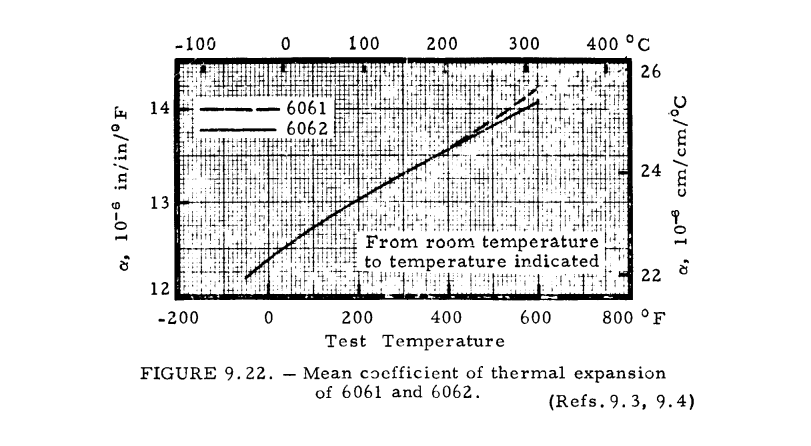
\includegraphics[width=0.8\textwidth]{Al_alpha_values}}
                \caption{Coefficient of thermal expansion of aluminum as a function of temperature}
                \label{fig:al_alpha}
            \end{figure}            
            
            Table \ref{fig:al_alpha} \cite{muraca1972aluminum} shows the change in $\alpha$ across the operating temperature range. As shown in the table, $\alpha$ changes constantly depending on the temperature. However the change in $\alpha$ from $T_{\text{ref}}$ to $T_{max}$ is very small and will only account for an error of a few microns which is well within the error range given in our design requirements.
            
            Using $\alpha = 22.7 \times 10^{-6} \frac{1}{\degC}$, we get the expected
            
            $\delta L {(T_{\text{ref}} \to T_{max})} = L_0 \alpha \Delta T = (84.335 \text{ mm})(22.7 \times 10^{-6})(70) = 0.1339 \text{ mm}$  
            
            To find the actual change in length based on a constant change in $\alpha$, we use the formula 
            \begin{align*}
            \Delta L &= L_0 \int_{T_1}^{T_2} \alpha(T) \, dT \\
            &= 84.335 \int_{10}^{80} (0.0058T + 22.6) \times 10^{-6} \, dT \\
            &= (84.335)\left[(0.0058(80)^2 + 22.6(80)) - (0.0058(10)^2 + 22.6(10))\right] \times 10^{-6} \\
            &= 0.1363 \text{ mm}
            \end{align*}

            The maximum error that will arise is at $T_{max}$ and $T_{min}$. The error is the difference between actual $\Delta L$ and expected $\Delta L$ which is

            $Error = \Delta L_{actual} - \Delta L_{expected} = 0.1363 \text{ mm} - 0.1339 \text{ mm} = 2.4 \text{ microns}$

            The 2.4 microns fall much below the error range of our design requirements so even added with the other errors that will occur in our system we will fall within the design requirements.
            Using the dimensional tolerance of $5 \mu m$ for $L_0$, we can combine these values as indicated in Table \ref{tab:act_specs_disc}:

            $$\sqrt{ \left( L_0 u_{\alpha} \right) ^2 + \left( \alpha u_{L_0} \right) ^2} = \sqrt{ \left( 84.335 * 2.4 \mu m \right) ^2 + \left( 23E-6 * 5 \mu m \right) ^2} = 0.2 \mu m \leq 0.3 \mu m$$


        \subsubsection{Specification 2: Reaction force deflection}
        \label{subsec:act_spec_2}

        The actuator must overcome resisting forces without deformation before expansion can be 
        translated into movement. The forces resisting actuator expansion include friction
        and other un-modeled losses in the actuator-valve system, as well as the spring force of
        the bellows. The below calculations show that any error caused by deflection is minimal
        and will not cause the system to fall outside of the design requirements.


  
\begin{table}[H]
    \centering
    \caption{Actuator variables}
    \label{tab:act_known_var}
    \renewcommand{\arraystretch}{1.4}
    \begin{tabularx}{\textwidth}{l X l}
        \toprule
        \textbf{Symbol} & \textbf{Description} & \textbf{Value} \\
        \midrule
        $L_0$ &
        Original actuator length &
        \SI{84.335}{mm}
        \\\addlinespace
        $\alpha$ &
        Thermal expansion coefficient (aluminum) &
        \SI{23.1e-6}{\per\celsius}
        \\\addlinespace
        $\Delta T_{\text{lower}}$ &
        Temperature change (lower bound) &
        \SI{-80}{\celsius}
        \\\addlinespace
        $\Delta T_{\text{upper}}$ &
        Temperature change (upper bound) &
        \SI{+60}{\celsius}
        \\\addlinespace
        $k$ &
        Bellows spring constant &
        \SI{630236}{N/m}
        \\\addlinespace
        $F_{\text{friction}}$ &
        Friction force (estimated) &
        \SI{3}{N}
        \\\addlinespace
        $w$ &
        Actuator face width &
        \SI{0.03}{m}
        \\\addlinespace
        $t$ &
        Actuator face thickness &
        \SI{0.03}{m}
        \\\addlinespace
        $E_{\text{Al}}$ &
        Young's modulus of aluminum &
        \SI{69}{GPa}
        \\\bottomrule
    \end{tabularx}
\end{table}

\noindent\textbf{Deflection Calculations}

\vspace{1em}
Unit conversion for spring constant:
\begin{equation}
    k = 3600\;\frac{\text{lbf}}{\text{in}}
      \times \frac{4.448\;\text{N}}{\text{lbf}}
      \times \frac{1\;\text{in}}{0.0254\;\text{m}}
      = 630{,}236\;\frac{\text{N}}{\text{m}}
\end{equation}

%------------------------------------------------------------

%------------------------------------------------------------

Displacement of the valve stem due to a temperature change $\Delta T$:
\begin{equation}
    \delta x = L_0 \cdot \alpha \cdot \Delta T
\end{equation}

Force exerted by the bellows spring opposing the displacement:
\begin{equation}
    F_{bellows} = k \cdot \delta x
\end{equation}

The total resistance the actuator must overcome is the sum of friction and bellows spring force.
Note that the largest contributor to friction force will be the sliding of the valve plates. As
the system is only required to adjust prior to testing, there will be no hydrogen flow and thus minimal
normal force pressing the plates together. Citing $F_{friction} = \mu*N $, we can assume friction force
will be minimal but include a worst-case value of 3N in calculations. This results in:
\begin{equation}
    F_{resistance} = F_{bellows} + F_{friction}
\end{equation}

This force is applied to the face of the actuator of area calculated:
\begin{equation}
    A_{contact} = w \cdot t
\end{equation}

The compressive or tensile stress on the actuator face:
\begin{equation}
    \sigma = \frac{F_{resistance}}{A_{contact}}
\end{equation}

Using Young's modulus (valid for both tension and compression in aluminum) to obtain strain:
\begin{equation}
    \varepsilon = \frac{\sigma}{E_{Al}}
\end{equation}

The elastic deformation of the actuator caused by the resisting force:
\begin{equation}
    \delta_{mech} = \varepsilon \cdot L_0
\end{equation}

The mechanical deflection as a percentage of the thermal displacement to 
quantify actuation error at temperature extrema:
\begin{equation}
    \%\,\text{error} = \frac{\delta_{mech}}{\delta x} \times 100\%
\end{equation}

%------------------------------------------------------------
\noindent\textbf{Results}
%------------------------------------------------------------

\begin{table}[h!]
\centering
\caption{Summary of results for upper and lower temperature bounds}
\vspace{0.5em}
\begin{tabular}{lSS}
\toprule
\textbf{Parameter} & \textbf{Lower Bound} & \textbf{Upper Bound} \\
                   & {($\Delta T = -80$\,\textdegree C)} & {($\Delta T = +60$\,\textdegree C)} \\
\midrule
$\delta x$ \textnormal{(m)}              & 2.6741e-4   & 1.0505e-4  \\
$F_{bellows}$ \textnormal{(N)}           & 168.6       & 66.2       \\
$F_{friction}$ \textnormal{(N)}          & 3.0         & 3.0        \\
$F_{resistance}$ \textnormal{(N)}        & 171.6       & 69.2       \\
$\sigma$ \textnormal{(MPa)}              & 0.191       & 0.077      \\
$\varepsilon$ \textnormal{(\textmu strain)} & 2.77     & 1.12       \\
$\delta_{mech}$ \textnormal{(m)}         & 2.33e-7     & 9.42e-8    \\
\%\,\textnormal{error}                   & 0.087       & 0.090      \\
\bottomrule
\end{tabular}
\end{table}

\noindent The mechanical deflection due to the resisting force is less than $0.1\%$ of the thermal
displacement in both cases, confirming that the net displacement is dominated by thermal
expansion and the resisting forces have negligible effect on actuator length.


        \subsection{Design Requirement Updates}
        \label{subsec:act_req_updates}

         Requirements for actuator operation have developed with further sub-requirements being 
        defined and individual weight being reevaluated by importance. Preliminary 
        conditions were defined by the need to deliver necessary stroke length for valve operation, 
        that thermal expansion
        should be precise and predictable, and that actuator length combined with other sub-system
        components should be contained within the mechanical envelope. The governing equation for
        the actuator expansion $\Delta L = L_o\Delta T\alpha $ relates expansion magnitude to 
        undeformed length $L_o$ and the linear coefficient of expansion $\alpha$. In preliminary 
        designs actuator length was maximized within the bounds of the mechanical envelope. 
        An amplifying interface between the valve stem and actuator was designed to increase 
        linear movement to the necessary stroke length via a compound gear train. This allowed the
        system to meet actuation distance needs of the valve while keeping within the mechanical 
        envelope. Discussion with subject matter experts and further calculations 
        showed that backlash and expected tolerance deviations from machining and assembly would
        be compounded by the gear train. 
        This would push the entire system out of error tolerance and 
        sparked consideration of eliminating the interface in favor of increasing un-deformed actuator
        length $L_o$. The increase in the weighted importance of precision led to discussion with
        our sponsor solidifying the mechanical envelope as a soft requirement. This allowed the actuator
        length to exceed the bounds of the mechanical envelope in interest of preserving movement precision.

        Though considered a "soft requirement", deviation outside of the mechanical envelope should still 
        be minimized. Further research was done into materials with higher coefficients of thermal 
        expansion to decrease necessary actuator length and it was found that zinc and magnesium alloys,
        as well as specialized polymers can exceed the expansion of aluminum. 
        Issues with these materials brought material property requirements
        to the forefront of our consideration regarding stability of mechanical properties across the operating temperature
        range. 



    \section{Mount Subsystem}

     \subsection{Overview}

            % Paragraph 1
            In the original Preliminary Design Report, we did not treat the mount as a subsystem requiring independent analysis. It was solely described as rigid structural frame whose function was to hold
            the actuator above the valve housing. In this detailed design phase, we realized that we needed to broaden our understanding of this design piece. The mount is not merely a structural bracket, but a dynamic
            element that responds to thermal changes and whose dimensional behavior directly affects the displacement delivered to the valve. 

            % Paragraph 2
            The crux of the matter is that the actuator block is anchored at the top interior face of the mount, and the free end extends downward to contact the valve stem. As the ambient temperature changes, the aluminum
            actuator expands or contracts the valve stem. However, the steel mount also expands or contracts over the same temperature range as it is nested above the housing. Since the mount and actuator share a common anchor point at the top, the displacement
            delivered to the valve is not the gross thermal expansion of the actuator alone. It is the difference between the actuator's expansion and the mount's expansion over the same vertical span. Therefore, the mount introduces another element of thermal
            expansion that directly affects the displacement that subtracts from the actuator's stroke. If this effect is not properly account for, the device can possibly under-stroke and the effective orifice diameter will fail to reach its specified endpoints.

            % Paragraph 3
            After realizing how error can cascade from the thermal expansion of the mount, it became crucial to identify subsystem-level design requirements. Within the mount, there are three careful considerations. First, the mount needs to be stiff enough such that its mechanical
            deflection under the actuator's reaction force is negligible compared to the total actuator stroke. Crucially, to resolve this issue our mount needs enough thickness. Second, the thermal expansion of the mount must be quantified and incorporated into the actuator length calculation.
            The required actuator length can have overshoot or undershoot negating the entire effects of the valve if the mount thermal expansion is not properly accounted for. Third, the mount must provide a calibration mechanism capable of setting the orifice to the correct effective diameter
            at the reference temperature of 25 $\degC$ with a resolution at least as fine as the $\pm$0.0127 mm tolerance on $D_{\text{eff}}$. This calibration must also withstand the clamping, thermal cycling, and full operating pressure without shifting. 

            These three requirements are the basis of the analysis presented in the following sections.

        

        \begin{table}[H]
            \centering
            \caption{Mount Specifications (repeated)}
            \mountSpecs
            \label{tab:mount_specs_disc}
        \end{table}
        \subsection{Specification Compliance}
        \subsubsection{Specification 1: Dimensional tolerances}
        \label{subsec:mount_spec_1}

        Table \ref{tab:mount_specs_disc} lists again the specifications from Section \ref{subsec:mount_sel_crit}

            The dimensions between the base of the mount and the upper interior, where the actuator will be mounted, are specified as 0.005 $\mu$m in the engineering drawings.

        \subsubsection{Specification 2: User calibration}
        \label{subsec:mount_spec_2}

            Shim washers are commonly used for micrometer-level height adjustments. After manufacturing, our team will be able to measure the exact dimensions of our parts tools available in the machine shop on campus.
            After calculation of the expected post-assembly value of $X(T_{\text{ref}})$, we can increase the height of the mount by one of three values:

            \begin{itemize}
                \item 100 $\mu m$ with the thick washer
                \item 10 $\mu m$ with the thin washer
                \item 110 $\mu m$ with both washers
            \end{itemize}

            depending on the measured tolerance values. Finally, we will add the crush washers, which provide reliable plastic compression to a tolerance of $5 \mu m$ over a range of $15 \mu m$.
            We will be able to tighten the screws with a torque wrench, compressing and plastically deforming the crush washers, to precisely bring the mount height down from a height of $15 \mu m$ above to within $5 \mu m$ above or below the target height. This complies with the specified range. 

        \subsubsection{Specification 3: Thermal expansion}
        \label{subsec:mount_spec_3}

            As the actuator expands with temperature, the mount will similarly expand, increasing $X(T_{\text{ref}})$ and detracting from the actuator's expansion.
            This must be kept below \mountdLTol\ as specified. The mount will be machined at $T_{\text{ref}}$, meaning its worst error will occur at $-60 \degC$.
            The thermal expansion of the mount can be calculated simply:

                $$\Delta L = L_0 \alpha \Delta T = \left( 122.476\ mm \right) \left( \SI{1.2e-6}{\per\celsius} \right) \left( -85 \degC \right) = -12.5\ \mu m$$

            This meets the specified deviation. Its implications are dealt with in Section \ref{subsec:sys_comp}.

        \subsubsection{Specification 4: Mechanical envelope}
        \label{subsec:mount_spec_4}

            As shown in Appendix \ref{app:drawings}, the mount subsystem's maximum mechanical envelope is
            \begin{itemize}
                \item Longitudinal: 100 mm. Its ends lie flush with the housing inlet and outlet faces.
                \item Lateral: 80 mm. Its sides also lie flush with the housing flanges.
                \item Vertical: 127.43 mm. This is the total height of the mount, which site on top of the housing flanges.
            \end{itemize}


       
        \subsection{Design Requirement Updates}
        \subsubsection{Trapezoidal Mount Plate Requirement Updates}
            The system-level mechanical envelope requirement was ($\leq$ 10 $cm^3$) and the stiffness requirement both roll down directly to the mount plates. The plates must be tall enough to house the actuator block in the cavity between them, wide enough such that the base can cradle the valve housing,
            and stiff enough such that deflection from the actuator's reaction force is negligible. 

        \subsection{Trapezoidal Mount Plate Current Implementation}
            The two trapezoidal mount plates are machined from Invar 36 stock. The plates rise vertically from the fixture and taper inward toward the top, forming the A-frame geometry visible in Figure \ref{fig:mount_cutaway_oblique}. The actuator fits in the cavity between the two plates with the upper end welded to the interior
            top face. Holes machined through the top of each plate provide access for the laser beam welding process that bonds the actuator to the mount. The large open windows on the sides provide access for laser welding the valve stem to the lower end of the actuator. These features were implemented in the design with manufacturing in mind.
            

             \begin{table}[H]
                \centering
                \caption{Mount Parameters}
                \label{tab:mount_parameters}
                \begin{tabularx}{\textwidth}{l X l}
                    \toprule
                    \textbf{Parameter} & \textbf{Description} & \textbf{Value} \\
                    \midrule
                    Material &
                    &
                    Invar 36
                        \\\addlinespace
                    $E$ &
                    Young's Modulus &
                    140 GPa
                    \\\addlinespace
                    $S_y$ &
                    Yield Strength &
                    240 MPa
                    \\\addlinespace
                    $\alpha_{Invar}$ &
                    CTE of Invar &
                    $1.20 \times 10^{-6} \, \degC ^{-1}$
                    \\\addlinespace
                    $H$ &
                    Mount height &
                    122.48 mm
                    \\\addlinespace
                    $\Delta{T}$ &
                    Operating temperature range &
                    85 $\degC$
                    \\\addlinespace
                    F &
                    Axial actuation force &
                    168.96 N
                    \\\bottomrule
                \end{tabularx}
            \end{table}           

        \subsubsection{Trapezoidal Mount Structural Stiffness}
        In addition to thermal expansion, the mount plate thickness is an important consideration. The plates must be thick enough such that the actuator's reaction force or response to pressure does not cause any mechanical deflection. The actuator exerts a maximum force
         of F = 168.96 N, which is the bellows spring force at full stroke, per Section \ref{subsec:valve_spec_1}. This force is reacted at the top of the mount and transmitted down through the two trapezoidal plates to the fixture. A detailed stiffness analysis using the machined cross-section geometry from the CAD model, or equivalently a finite element analysis under the 168.96 N reaction load, is planned for the spring quarter model validation phase. 
         Given that Invar 36 has a modulus of 140 GPa and the mount plates have substantial cross-sectional area at their base, the deflection under such a modest load is expected to be negligible relative to the 162 µm stroke from $T_{\text{ref}}$, but this will be quantitatively confirmed before fabrication.
        
        \subsubsection{Fasteners Design Requirement Updates}
        The fastener joints must maintain a sufficient enough clamping force across the full operating temperature range. Any discrepancy between the fasteners and the fixture corrupts the calibration of the entire device.

        \subsubsection{Fasteners Current Implementation}
        Eight M5 black-oxide alloy steel socket head screws secure the mount plates to the fixture. The valve housing and calibration shim stack are clamped between these screws. Each screw passes through the mount from the top, through the washer calibration stack, over the housing, and threads into the fixture at the base.
        A standard 18-8 M5 stainless steel oversized washer sits under each screw head to distribute the clamping load across the mount plate surface. 
        
        \begin{table}[H]
                \centering
                \caption{Fastener Parameters}
                \label{tab:fastener_parameters}
                \begin{tabularx}{\textwidth}{l X l}
                    \toprule
                    \textbf{Parameter} & \textbf{Description} & \textbf{Value} \\
                    \midrule
                    Fastener &
                    M5 Black-oxide alloy steel socket head screw &
                    McMaster 91290A254
                        \\\addlinespace
                    $A_t$ &
                    Tensile stress area &
                    14.1$mm^2$
                    \\\addlinespace
                    $S_p$ &
                    Proof load stress &
                    970 MPa
                    \\\addlinespace
                    $\alpha_{Invar}$ &
                    CTE of Invar &
                    $1.20 \times 10^{-6} \, \degC^{-1}$
                    \\\addlinespace
                    $H$ &
                    Mount height &
                    88.9 mm
                    \\\addlinespace
                    $\alpha_{Aluminum}$ &
                    CTE of aluminum actuator &
                    $23.6 \times 10^{-6} \, \degC$
                        \\\addlinespace
                    $\Delta{T}$ &
                    Max displacement from reference &
                    85 $\degC$
                    \\\addlinespace
                    F &
                    Axial actuation force &
                    168.96 N
                    \\\bottomrule
                \end{tabularx}
            \end{table}

        Using the proof load equation, we can calculate the total capacity of force for the joint:
        \[ F_{bolt} = A_t \times S_p \]
        Plugging in the values from the table:
        \[ F_{bolt} = \SI{14.2e-6}{\metre\squared} \times 970 \times {MN/m^2} = 13.774 \ \text{kN} \]

        For a total of eight screws:
         \[ F_{total} = 8 \times \SI{14.2e-6}{\metre\squared} \times 970 \times {MN/m^2} = 110.192 \ \text{kN} \]

        The maximum external separating load on the joint is the actuator force of 168.96 N. The factor of safety against the joint separation is:
        \[ FOS_{bolt} = F_{total} / F = 81.5 \]
        
        The bolted joint is more than capable of receiving the actuator load. The M5 fastener size was selected not for the structural necessity but for standardization, ease of assembly, and compatibility with the shim washer stack geometry.

        \subsubsection{Fasteners Preload Stability}
        The fasteners (alloy steel, \( \alpha \approx 11.5 \times 10^{-6} /^\circ\text{C} \)) pass through the Invar 36 mount plates (\( \alpha = 1.30 \times 10^{-6} /^\circ\text{C} \)), 
        the steel shim washers (\( \alpha \approx 12.0 \times 10^{-6} /^\circ\text{C} \)), and thread into the fixture. The CTE mismatch between the fastener and the Invar mount means the bolt will expand more than the clamped material over the joint grip length. 
        The worst-case thermal preload shift occurs at the cold extreme of \( -60^\circ\text{C} \), representing \( \Delta T = 85^\circ\text{C} \) below the reference. For a grip length on the order of \( 25 \text{ mm} \), the differential expansion between the bolt and the Invar is:
        \(\Delta\delta = L_{\text{grip}} \cdot (\alpha_{\text{bolt}} - \alpha_{\text{Invar}}) \cdot \Delta T = 25 \times (11.5 - 1.30) \times 10^{-6} \times 85 \approx 0.022 \text{ mm} = 22 \text{ µm}\)

        This $22 \, \mu\text{m}$ of differential expansion will slightly increase bolt preload at low temperatures and slightly decrease it at elevated temperatures. 
        Given that the proof load per bolt ($13.774 \ \text{kN}$) exceeds the per-bolt share of the actuator load ($168.96 / 8 \approx 21.1 \, \text{N}$) by a factor of $6.52 \times 10^8$, this preload variation does not threaten joint integrity. 




        % \subsection{Calibration Stack}
        % \subsection{Fasteners}
        





    

    \section{Subsystem Interaction}
    
   
    The three subsystems of the PTCD form an open-loop control chain as depicted in Figure \ref{fig:controls_diagram}. Each subsystem has inputs within the system transfer function, and the interactions between them define the net behavior of the device. This section describes the mechanical and thermal interfaces between subsystems and identifies the coupling effects that each must account for.
    
    \subsection{Mount–Actuator Interface}
    The actuator block is welded to the interior top face of the mount. This weld joint defines the fixed boundary condition from which the actuator expands downward. Because both the mount and actuator are exposed to the same ambient temperature, both undergo thermal expansion simultaneously. The mount expands downward from its anchor at the fixture toward the valve, while the actuator expands downward from its anchor at the top of the mount toward the valve stem. 
    These two expansions oppose one another: the mount's growth effectively raises the actuator's anchor point relative to the valve housing, reducing the net stroke delivered to the valve. The net displacement is therefore:
    $$ \delta_{\text{net}} = L_{\text{act}} \cdot \alpha_{\text{Al}} \cdot \Delta T - H_{\text{mount}} \cdot \alpha_{\text{Invar}} \cdot \Delta T $$
    The selection of Invar 36 for the mount minimizes the opposing direction of expansion. At $-60\,^\circ\text{C}$, the mount contributes only $\alpha_{\text{Invar}} \cdot H \cdot \Delta T = (1.2 \times 10^{-6})(88.9)(85) \approx 9.1\,\mu\text{m}$ of opposing displacement, 
    compared to the actuator's expansion of approximately $162\,\mu\text{m}$ over the same interval. The actuator length $L_0 = 84.335\,\text{mm}$ was sized to deliver the required net stroke after subtracting this mount expansion.

    \subsection{Actuator–Valve Interface}
    The lower end of the actuator is laser welded directly to the valve stem. This rigid connection transmits the actuator's thermal displacement to the translating orifice plate with a unity gain of $dX/dL = 1$. The displacement delivered by the actuator is identically the displacement received by the valve plate. This direct coupling eliminates backlash and hysteresis that would arise from 
    intermediate mechanical interfaces. However, it also means that the valve's reaction force is transmitted directly back into the actuator. The bellows spring force of $F_s = 168.96\,\text{N}$ at full stroke compresses the 
    actuator axially. This deflection is negligible, but is carried upward through the actuator into the mount. This must be stiff enough to absorb it without measurable deflection of its own.

    \subsection{Mount–Valve Interface} 
    The mount sits on top of the valve housing, separated by the calibration shim stack. The vertical distance from the interior top face of the mount to the orifice plate defines the reference offset $X(T_{\text{ref}})$. This distance governs the constant $A_0$ in: $$\requiredRelationship$$ The shim washers between the mount and housing enable 
    adjustment during final assembly to bring $X(T_{\text{ref}})$ within the specified $\pm 5\,\mu\text{m}$ of its target value. The eight M5 fasteners clamp the mount, shim stack, and housing together as a rigid unit, ensuring 
    that the calibrated offset does not shift under thermal cycling or the actuator's reaction load.

    \subsection{Thermal Coupling}
    \label{subsec:sub_int}

    All three subsystems are exposed to the ambient air temperature, which is the sole input to the control system. The valve housing thermally isolates the actuator from the internal gas flow. The $10\,\text{mm}$ steel 
    wall thickness ensures that the potential temperature difference between the gas and the ambient air does not propagate to the actuator. The valve stem, fabricated from Invar 36, provides 
    additional thermal resistance between the pressurized interior and the actuator. 



    \section{System Compliance}
    \label{subsec:sys_comp}

        Recall that the system transfer function is 
        
        $\transferFunction$ \quad (eq. \ref{eq: transfer_function})
        
        which must equal the required relationship

        $\requiredRelationship$ \quad (eq. \ref{eq: required_relationship})

        to the given tolerance. Let us consider the worst-case scenario in which each core responsibility is at the maximum limit of tolerable error.
        The error in height of the orifice, X(T), is the sum of the greatest errors in the system. We have calculated the following dimensional or operational deviations throughout the Discussion:
        
        \begin{itemize}
            \item The height of the mount from drawing M2: $122.476\,{}^{+0}_{-0.01} mm$
            \item The length of the actuator from drawing A1: $84.335 \pm 0.005mm$
            \item The thermal expansion error of the actuator: $162.35\,{}^{+2.4}_{-0} \mu m$
            \item Actuator compression due to bellows force (this will be in the opposite direction of the other deviations, cancelling them partially): $0.3 \mu m$
            \item Valve stem compression due to bellows force (this will also negate the other error values): $5 \mu m$
            \item The dimensional length of the valve stem (because the tolerance only allows the length to err too short, this will also detract from the total error): $24.041\,{}^{+0}_{-0.01} mm$
            \item Most significantly, the thermal expansion of the mount will decrease the orifice height by: $12.5 \mu m$
        \end{itemize}

        These sum up to 
        $(10 + 5 + 2.4 - 0.3 - 5 - 10 - 12.5) = -10.4 \mu m$

        Because $D_{\text{effective}} = \sqrt{\frac{2}{\pi}}*X(T)$, the maximum error in the Required Relationship, according to these specifications, is
        $\sqrt{\frac{2}{\pi}}*(10.4 \mu m) = 8.3 \mu m$. This is within the tolerance specification for all temperatures.
        As stated in Section \ref{sec:initial_system_requirements} and Appendix \ref{app:errorProp}, the minimum tolerance is 12.7 $\mu$m.
        This leaves enough room for unseen errors.

        Note that this calculation makes a number of first-order assumptions, which will be refined early next quarter as the computational model is optimized.
        These assumptions included the following:

        \begin{itemize}
            \item The square orifice will have a negligible fillet radius via high-precision manufacturing techniques. These methods will be researched in the coming weeks.
            \item The thermal expansion of the valve housing will be negligible.
            \item Several dimensional tolerances were ignored.
        \end{itemize}

        However, this provides a first-order approximation that if this iteration is not within tolerance, it will at least be close.
        
        % \begin{table}[H]
        %     \centering
        %     \caption{Control derivative tolerances}
        %     \label{tab:tol_final}
        %     \begin{tabular}{cc}
        %         \toprule
        %         $\frac{dD}{dX} = -\sqrt{\frac{2}{\pi}} \pm \dDdXTol$ \\
        %         $\frac{dX}{dL} = 1 \pm \dXdLTol$ \\
        %         $\frac{dL}{dT} = \sqrt{\frac{\pi}{2}} A_1$ \\
        %         $ dud $ \\
        %         \bottomrule
        %     \end{tabular}
        % \end{table}

            


    
% ============================================================================
% SECTION 4: PRELIMINARY BILL OF MATERIALS
% ============================================================================
% GRADING: Section V — 10 points
%   "All parts included, each part belongs to a sub system,
%    accurate costs, all info included"
%
% TEMPLATE GUIDANCE:
%   - TABLE FORMAT (mandatory)
%   - Include: part numbers, part names, quantity, material,
%     purchased vs fabricated, supplier name/part number if purchased
%   - For fabricated parts: size and cost of raw material
%   - Include any special tooling that must be purchased
%   - Must be complete enough to release your budget for Spring quarter
%
% ESTIMATED LENGTH: 1-2 pages
%
% TIP: The longtable environment is used here because the BOM may
% span multiple pages. Regular tabular would break across pages poorly.
% ============================================================================

\chapter{Preliminary Bill of Materials}
\label{sec:bom}

%--- BEGIN CONTENT ---

    Sandia National Labs awarded our team \$2,000 to manufacture and test a prototype of the \device.
    Due to the extreme precision and conditions required for our design, the prototype will serve as a first-order approximation to the real device.
    SNL explicitly gave us no budget cap for the final design package, giving us liberty to recommend more expensive and exotic materials, manufacturing methods, and testing procedures after we test this cheaper prototype next quarter.
    Note that this bill of materials (BOM) covers material costs only and remains subject to revision. Funds for the project were awarded in close proximity to the report's due date allowing for manufacturer selection to be completed early next quarter. The team is actively engaged with manufacturers to obtain quotes for the precision machining required for several components. 
    These manufacturing costs, along with testing apparatus procurement, will constitute the remainder of the projected budget. The total cost presented here should therefore be considered a preliminary estimate, with the final project 
    cost to be updated upon receipt of manufacturing quotes early next quarter.

    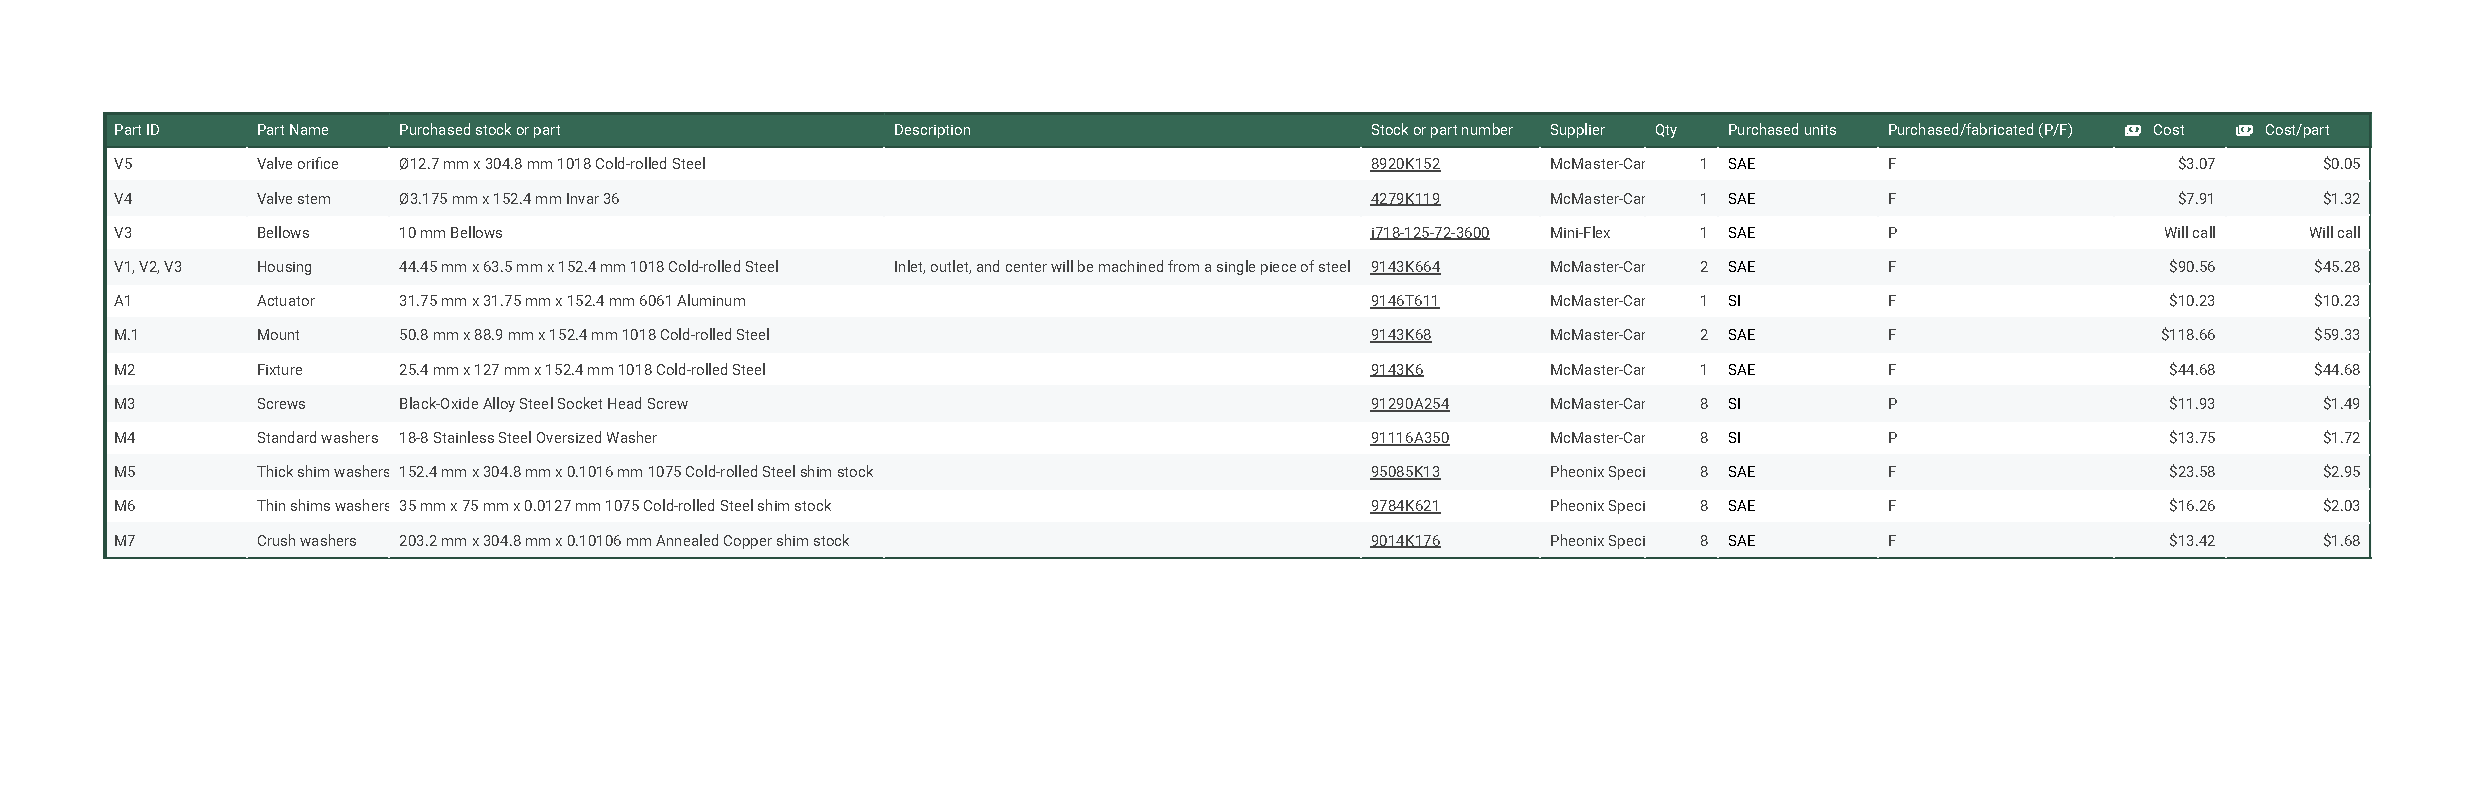
\includepdf[pages=1, fitpaper=true, landscape=true]{BOM.pdf}


%--- END CONTENT ---


% ============================================================================
% SECTION 5: PROJECT MANAGEMENT INFORMATION
% ============================================================================
% GRADING: Section VI — 15 points total
%   6.1) Appropriate tasks identified over 2 quarters (5.0 pts)
%   6.2) Updated Gantt chart for 2 quarters (5.0 pts)
%   6.3) Critical path method (CPM) analysis (5.0 pts)
%
% TEMPLATE GUIDANCE:
%   - Task list must be specific to YOUR project and design
%   - Gantt chart must span BOTH quarters (Fall through Spring)
%   - CPM must be in graphical format with a paragraph description
%   - If permits or PE sign-offs are needed, note them here
%
% ESTIMATED LENGTH: 3-4 pages (could be longer)
% ============================================================================

\chapter{Project Management Information}
\label{sec:project_management}


% --- 5.1: Task List ---
\section{Updated Task List}
\label{subsec:task_list}

%--- BEGIN CONTENT ---

\begin{table}[h]
\caption{Task List for Winter and Spring Quarters}
\centering
\begin{tabular}{@{} c l @{}}
\toprule
\textbf{\#} & \textbf{Task Description} \\
\midrule
\multicolumn{2}{c}{\textbf{Winter Quarter}} \\
\midrule
1  & Prepare Questions for Sponsors \\
2  & First Memo Report \\
3  & Sponsor Meeting (Recurring) \\
4  & Define Problem Statement \\
5  & Research Potential Solutions \\
6  & Second Memo Report \\
7  & Fully Define Design Space \\
8  & Third Memo Report \\
9  & Problem Statement \\
10 & Project Specifications \\
11 & Presentation of Alternative Solutions \\
12 & Preliminary Calculations \\
13 & Final Designs \\
14 & Report Revision \\
15 & Subsystem Delegation \& Communication \\
16 & Performance Calculations \\
17 & Design Refinement \\
18 & Establish Sub-component Geometry \\
19 & CAD \\
20 & Fourth Memo Report \\
21 & Subsystem Integration \& Team Coordination \\
22 & Finalize Machine Architecture \\
23 & System Architecture \\
24 & Discussion \\
25 & Project Management \\
26 & Bill of Materials \\
27 & Abstract \\
28 & Report Revision \& Submission \\
\bottomrule
\end{tabular}
\end{table}

\newpage

\begin{table}[h]
\centering
\begin{tabular}{@{} c l @{}}
\toprule
\textbf{\#} & \textbf{Task Description} \\
\midrule
\multicolumn{2}{c}{\textbf{Spring Quarter}} \\
\midrule
29 & Assess Manufacturable Components \\
30 & Order Materials \\
31 & Sponsor Preliminary Design Review \\
32 & Tolerance Stack-up Analysis \\
33 & CAD Revisions \\
34 & FEA (Actuator, Valve, Gears) \\
35 & CFD (Valve) \\
36 & Thermal Analysis \\
37 & Design Revision \\
38 & Safety/Risk Assessment \\
39 & Rapid Prototyping/Machining \\
40 & Finish POC Model \\
41 & Complete Product Demonstration \\
42 & Draft Poster Design \\
43 & Final Report \\
44 & Final Poster Design \\
45 & Critical Design Reviews \\
46 & Design Showcase \\
\bottomrule
\end{tabular}
\end{table}

%--- END CONTENT ---


% --- 5.2: Gantt Chart ---
\section{Gantt Chart}
\label{subsec:gantt}

%--- BEGIN CONTENT ---
    An updated Gantt chart is provided below, spanning both the Winter and Spring quarters. 
    The chart includes all major tasks and milestones identified in the task list, with dependencies clearly indicated. 
    The vertical line represents the current date.

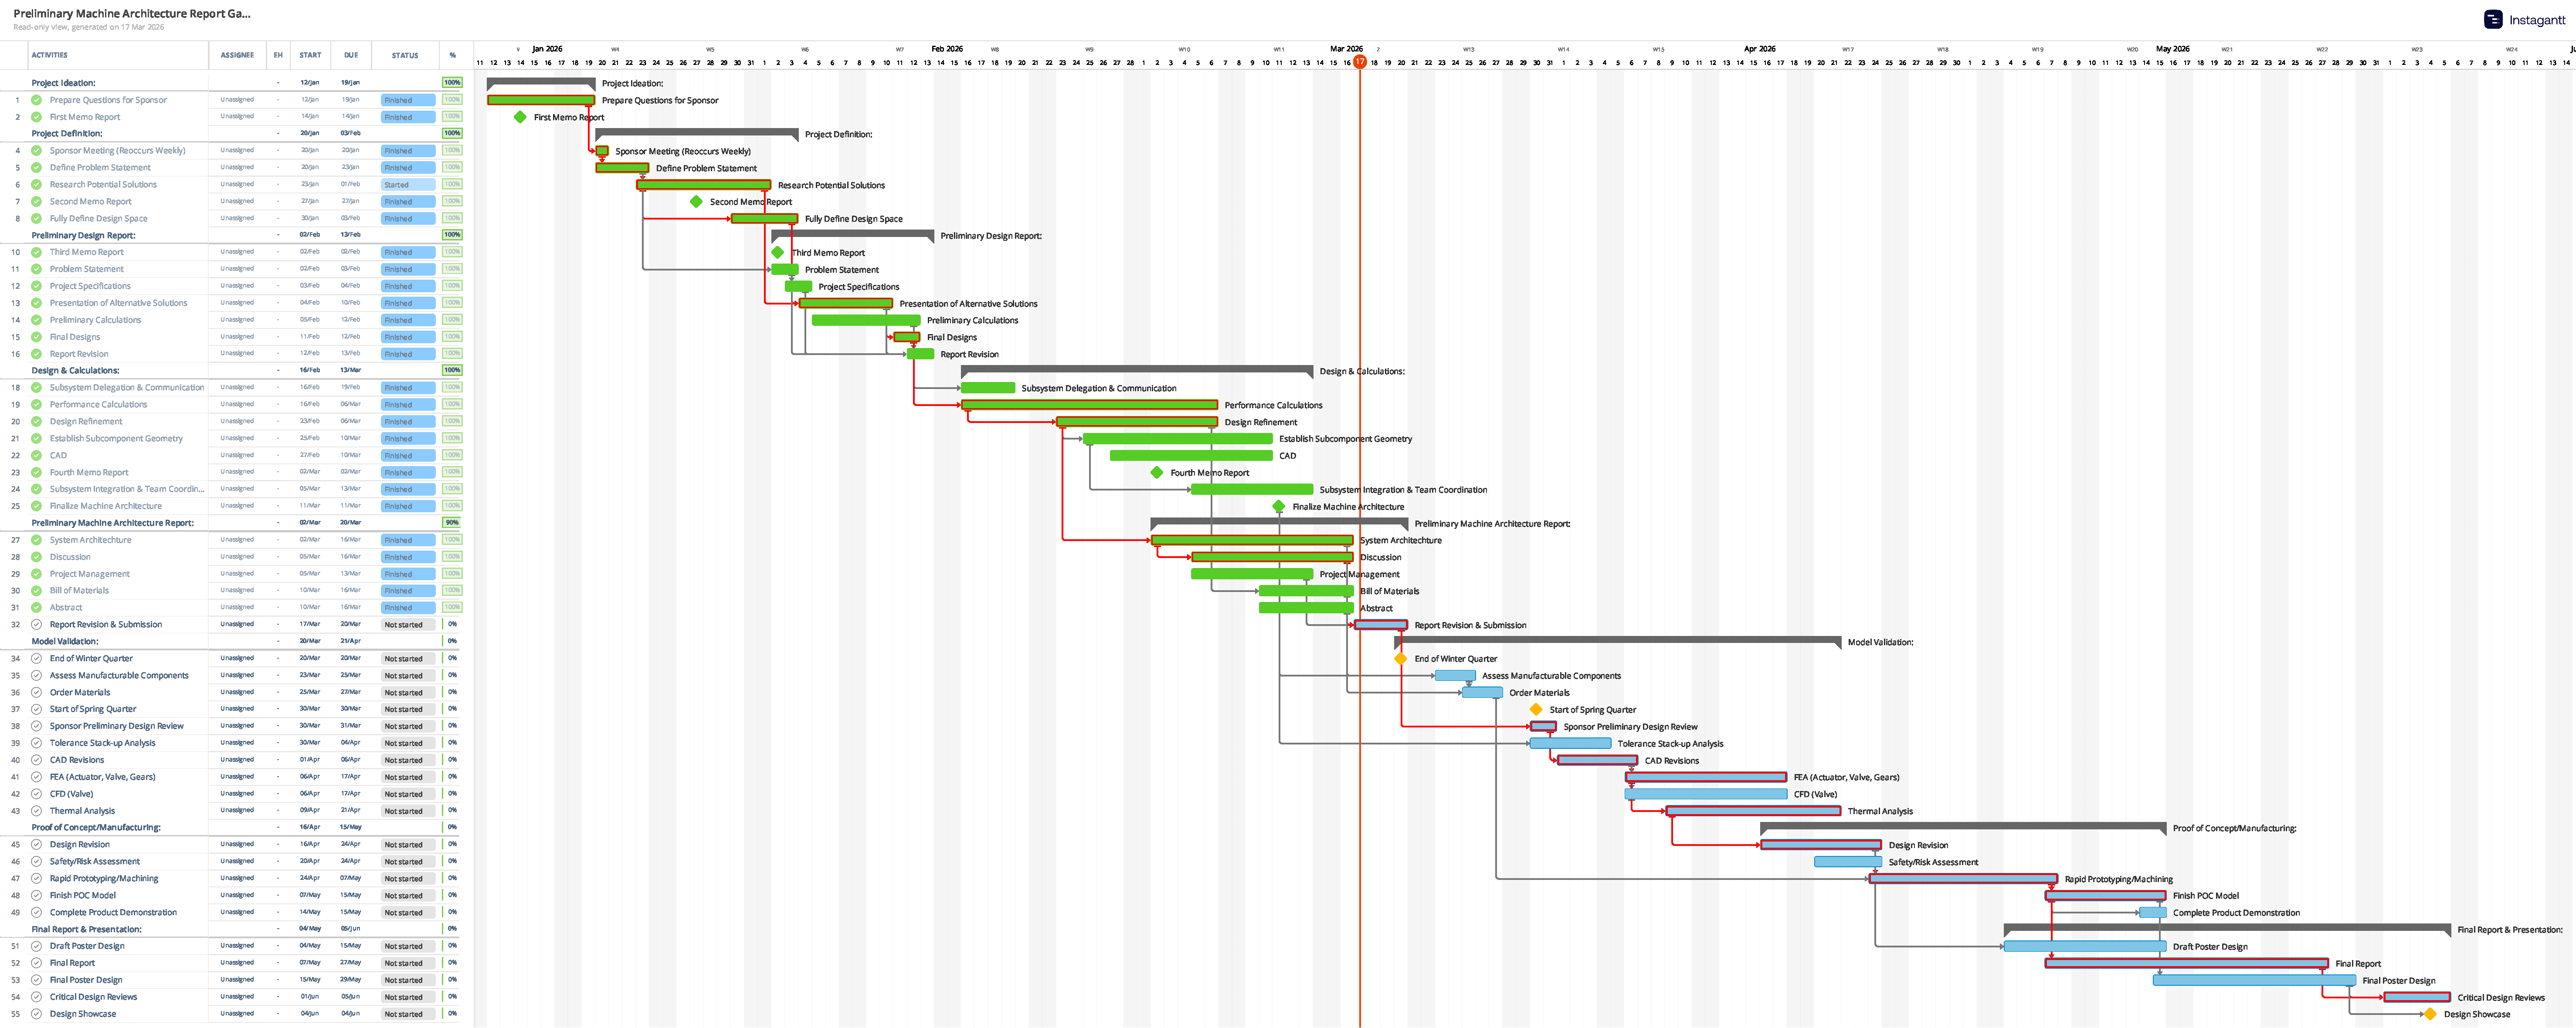
\includepdf[pages=1, fitpaper=true, landscape=true]{GanttChart.pdf}

%--- END CONTENT ---


% --- 5.3: Critical Path Method (CPM) Analysis ---
\section{Critical Path Method (CPM) Analysis}
\label{subsec:cpm}

%--- BEGIN CONTENT ---

The critical path, highlighted in red within the project Gantt chart, identifies the sequence of tasks with zero float that dictate the 
project’s minimum duration. This path began with the fundamental tasks of sponsor communication and problem statement definition, which
 were imperative for establishing the project's technical direction. These initial phases directly fed into the research and scoring of 
 alternative solutions, which provided the necessary data to begin performance calculations and design refinement. The analysis identifies
  a high-dependency transition point where the system architecture and design discussion were compiled for sponsor review; the subsequent 
  CAD revisions and computer modeling are entirely dependent on this feedback loop. Consequently, any delay in these design iterations would
   directly postpone the prototyping of the conceptual model and the completion of the final report. The project concludes with the Critical
    Design Review, which serves as the final milestone on the critical path, ensuring all technical requirements and documentation converge
     for the successful closeout of the project.

%--- END CONTENT ---


% ============================================================================
% SECTION 6: CITED REFERENCES
% ============================================================================
% GRADING: Part of Section I (General Considerations)
%   "Appropriate technical references" and "professional in appearance"
%
% TEMPLATE GUIDANCE:
%   - Use citations as appropriate for technical writing
%   - Cite other's work, supporting assumptions, technical data
%   - Use a consistent format (IEEE, APA, MLA — pick one)
%
% HOW THIS WORKS IN LATEX:
%   Option A (recommended): Use BibTeX with a .bib file.
%   Option B (simpler): Use thebibliography environment (shown below).
%
%   For Option A, create a file called "references.bib" with entries like:
%     @article{bon2025,
%       author  = {Bon, Bradley},
%       title   = {Passive Flow Control for Hydrogen Systems},
%       journal = {Sandia Technical Report},
%       year    = {2025}
%     }
%   Then cite with: \cite{bon2025}
%   And compile with: pdflatex -> bibtex -> pdflatex -> pdflatex
% ============================================================================

% \chapter{Cited References}
% \label{sec:references}

% --- Option B: Manual bibliography (simpler, no .bib file needed) ---
% Each \bibitem{key} creates a reference. Cite with \cite{key} in text.
%
% The [99] tells LaTeX the widest label will be two digits.

\begin{thebibliography}{99}

    \bibitem{ref_sandiaprompt}
    B.\ Bon,
    ``Passive Temperature Compensation Device --- Project Prompt,''
    Sandia National Laboratories, SAND2025-15446O, 2025.

    \bibitem{asme_b313}
    American Society of Mechanical Engineers, \textit{ASME B31.3: Process Piping}, 
    ASME, New York, NY, 2022.

    \bibitem{steen2010laser}
    W. M. Steen and J. Mazumder, \textit{Laser Material Processing}, 4th ed., 
    Springer, London, UK, 2010.

    \bibitem{aws2020welding}
    American Welding Society, \textit{AWS D1.1/D1.1M: Structural Welding Code --- Steel}, 
    AWS, Miami, FL, 2020.

    \bibitem{miniflex_design}
    Mini-Flex Corporation, \textit{Metal bellows Design Guide}, Mini-Flex Corporation, 
    Watervliet, NY. [Online]. Available: \url{https://mini-flex.com/metal-bellows-design-guide/}
    [Accessed: Mar. 2026].

    \bibitem{muraca1972aluminum}
    R.\ F.\ Muraca and J.\ S.\ Whittick,
    \textit{Materials Data Handbook: Aluminum Alloy 6061}, 2nd ed.,
    Western Applied Research \& Development, Inc.,
    NASA CR-123772, May 1972.
    Available: \url{https://ntrs.nasa.gov/api/citations/19720022808/downloads/19720022808.pdf}
    [Accessed: Mar. 2026].

    \bibitem{matweb}
    MatWeb, LLC, \textit{MatWeb Material Property Data}, 
    [Online]. Available: \url{https://www.matweb.com}, 
    Accessed: March 20, 2026.

    \bibitem{ref_Nise}
    N. S. Nise, Control Systems Engineering, 8th ed. Hoboken, NJ: Wiley, 2019.

    \bibitem{ref_Figliola}
    R. S. Figliola and D. E. Beasley, Theory and Design for Mechanical Measurements, 7th ed. Hoboken, NJ: Wiley, 2020, pp. 172–175.

    \bibitem{ref_carpentertechnology}
    Carpenter Technology Corporation, "Invar 36," Material Safety Data Sheet. \url{https://www.carpentertechnology.com/hubfs/7407324/Material%20Saftey%20Data%20Sheets/Invar%2036.pdf.}
    [Accessed: Mar. 20, 2026].
   
    \bibitem{ref_AZoM}
     AZoM, "Properties: Invar — Nickel Iron Alloy," AZoM.com. \url{https://www.azom.com/properties.aspx?ArticleID=515.}
    [Accessed: Mar. 20, 2026].

    \bibitem{ref_AircraftMaterials}
    Aircraft Materials Ltd., "Invar 36 / Nilo 36 / Alloy 36 (ASTM F1684)," AircraftMaterials.com. \url{https://www.aircraftmaterials.com/data/nickel/al36.html. }
    [Accessed: Mar. 20, 2026].

    \bibitem{ref_ISO}
    International Organization for Standardization, "Mechanical properties of fasteners made of carbon steel and alloy steel — 
    Part 1: Bolts, screws and studs with specified property classes — Coarse thread and fine pitch thread," ISO 898-1:2013, Geneva, Switzerland, 2013.

    \bibitem{ref_ASM}
    ASM International, Properties and Selection: Irons, Steels, and High-Performance Alloys, ASM Handbook, vol. 1. Materials Park, OH, USA: ASM International, 1993.
    

    



    % Add more \bibitem entries as needed.
    % In the body text, cite as: \cite{ref_sandiaprompt}

\end{thebibliography}


% ============================================================================
% APPENDICES
% ============================================================================
% TEMPLATE GUIDANCE:
%   - Label and title every appendix
%   - You MUST refer to each appendix in the body of the report
%   - Include: working drawings, product sheets, price quotes,
%     updated requirements table, scoring matrices, etc.
%
% IMPORTANT: Appendices don't count toward estimated page lengths
% of other sections, so put detailed tables and drawings here.
% ============================================================================

\newpage
\begin{appendices}

% --- Appendix A: Final Design Requirements ---
\chapter{Final Design Requirements}
\label{app:requirements}

    Below is a complete rolldown of the system requirements into subsystem specifications
    as previously listed in Tables \ref{tab:valve_specs}, \ref{tab:act_specs}, and \ref{tab:mount_specs}.

    Remember that the chief objective of the \device\ is to satisfy the Required Relationship:

        $$D_{\text{eff}} = A_1(T - T_{\text{ref}}) + A_0$$

    which corresponds to the system transfer function in equation \ref{eq: transfer_function}:

        $$D_{\text{eff}}=\frac{dD_{\text{eff}}}{dX} \left[\frac{dL}{dT}\frac{dX}{dL}(T-T_{\text{ref}})+X\left(T_{\text{ref}} \right) \right]$$

    while the secondary, soft requirement is to remain within the 10 cm x 10 cm x 10 cm Mechanical Envelope.


\newpage
\enlargethispage{4cm}
\begin{table}[H]
    \centering
    \caption{System-Level Requirements and Specification Rolldown}
    \label{tab:system_specs}
    \renewcommand{\arraystretch}{1.4}
    \begin{tabular}{|m{0.2\textwidth}|m{0.3\textwidth}|m{0.4\textwidth}|}

        \hline
        \textbf{System requirement}
            &
        \textbf{Core responsibility}
            &
        \textbf{Specification} \\

        \hline

        % ---- RR block ----
        \multirow[c]{9}{0.2\textwidth}{%
            \device\ must satisfy the Required Relationship:
            $D_{\text{eff}} = A_1(T - T_{\text{ref}}) + A_0$
        }
            &
        Valve orifice must govern $\frac{dD_{\text{eff}}}{dX} = \sqrt{\frac{2}{\pi}}$ to within \dDdXTol\
            &
        Maintain all dimensional tolerances to $-1\ \mu m$ where specified in drawings V4 and V5
        \\ \cline{2-3}

            &
        Valve stem must govern $\frac{dX}{dL} = 1$ to within \dXdLTol\
            &
        Must limit total thermal expansion and forced compression to \dXdLTol
        \\ \cline{2-3}

            &
        \multirow[c]{2}{0.3\textwidth}{%
            bellows must not change $\frac{dL}{dT}$ by more than \dLdTTolValve\ %
        }
            &
        Prevent a temperature gradient of less than \dTTol\ between the internal gas and the actuator contact point
        \\ \cline{3-3}

            &
            &
        Prevent a reaction force of more than \FTolValve
        \\ \cline{2-3}

        &
        Valve housing must prevent critical failure by rupture
        &
        Withstand a minimum of 10{,}000 psi internal pressure
        \\ \cline{2-3}

            &
        Actuator must govern $\frac{dL}{dT} = \sqrt{\frac{\pi}{2}} A_1$ to within \dLdTTolAct\
            &
        Limit the error of $\alpha$ and $L_0$ such that
        $\sqrt{(L_0 u_\alpha)^2 + (\alpha u_{L_0})^2} \leq $\dLdTTolAct
        \\ \cline{2-3}

            &
        \multirow[c]{3}{0.3\textwidth}{%
            Mount must fix $X(T_{\text{ref}}) = \sqrt{\frac{2}{\pi}} A_0$ %
        }
            &
        Maintain all dimensional tolerances to $0.005\ \mu m$ where specified in drawing M2
        \\ \cline{3-3}

            &
            &
        Allow adjustment from within \calRange\ above target to within \calTol\ of target
        \\ \cline{3-3}

            &
            &
        Limit thermal expansion to \mountdLTol
        \\ \hline

        % ---- ME block ----
        \multirow[c]{2}{0.2\textwidth}{%
            \device\ must remain approximately within the Mechanical Envelope
        }
            &
        Valve must not exceed its portion of the ME
            &
        Must not exceed \valveMEX\ lateral, \valveMEY\ vertical, \valveMEZ\ longitudinal mechanical envelope
        \\ \cline{2-3}

            &
        Mount must not exceed its portion of the ME
            &
        Must not exceed \mountMEX\ lateral, \mountMEY\ vertical, \mountMEZ\ longitudinal mechanical envelope
        
        \\ \hline

    \end{tabular}
\end{table}

$\left( \text{Equation\ \ref{eq: transfer_function}, for reference:} D = \frac{dD}{dX} \left[ \frac{dL}{dT} \frac{dX}{dL} \Delta T + X_0 \right] \right)$

% --- Appendix B: Engineering Drawing Package ---
\chapter{Engineering Drawing Package}
\label{app:drawings}

To manufacture the \device , refer to the following part and assembly drawings.
Pay special heed to the specified tolerances; as elaborated in this report, these must be satisfied to maintain the Required Relationship to its specified tolerance.

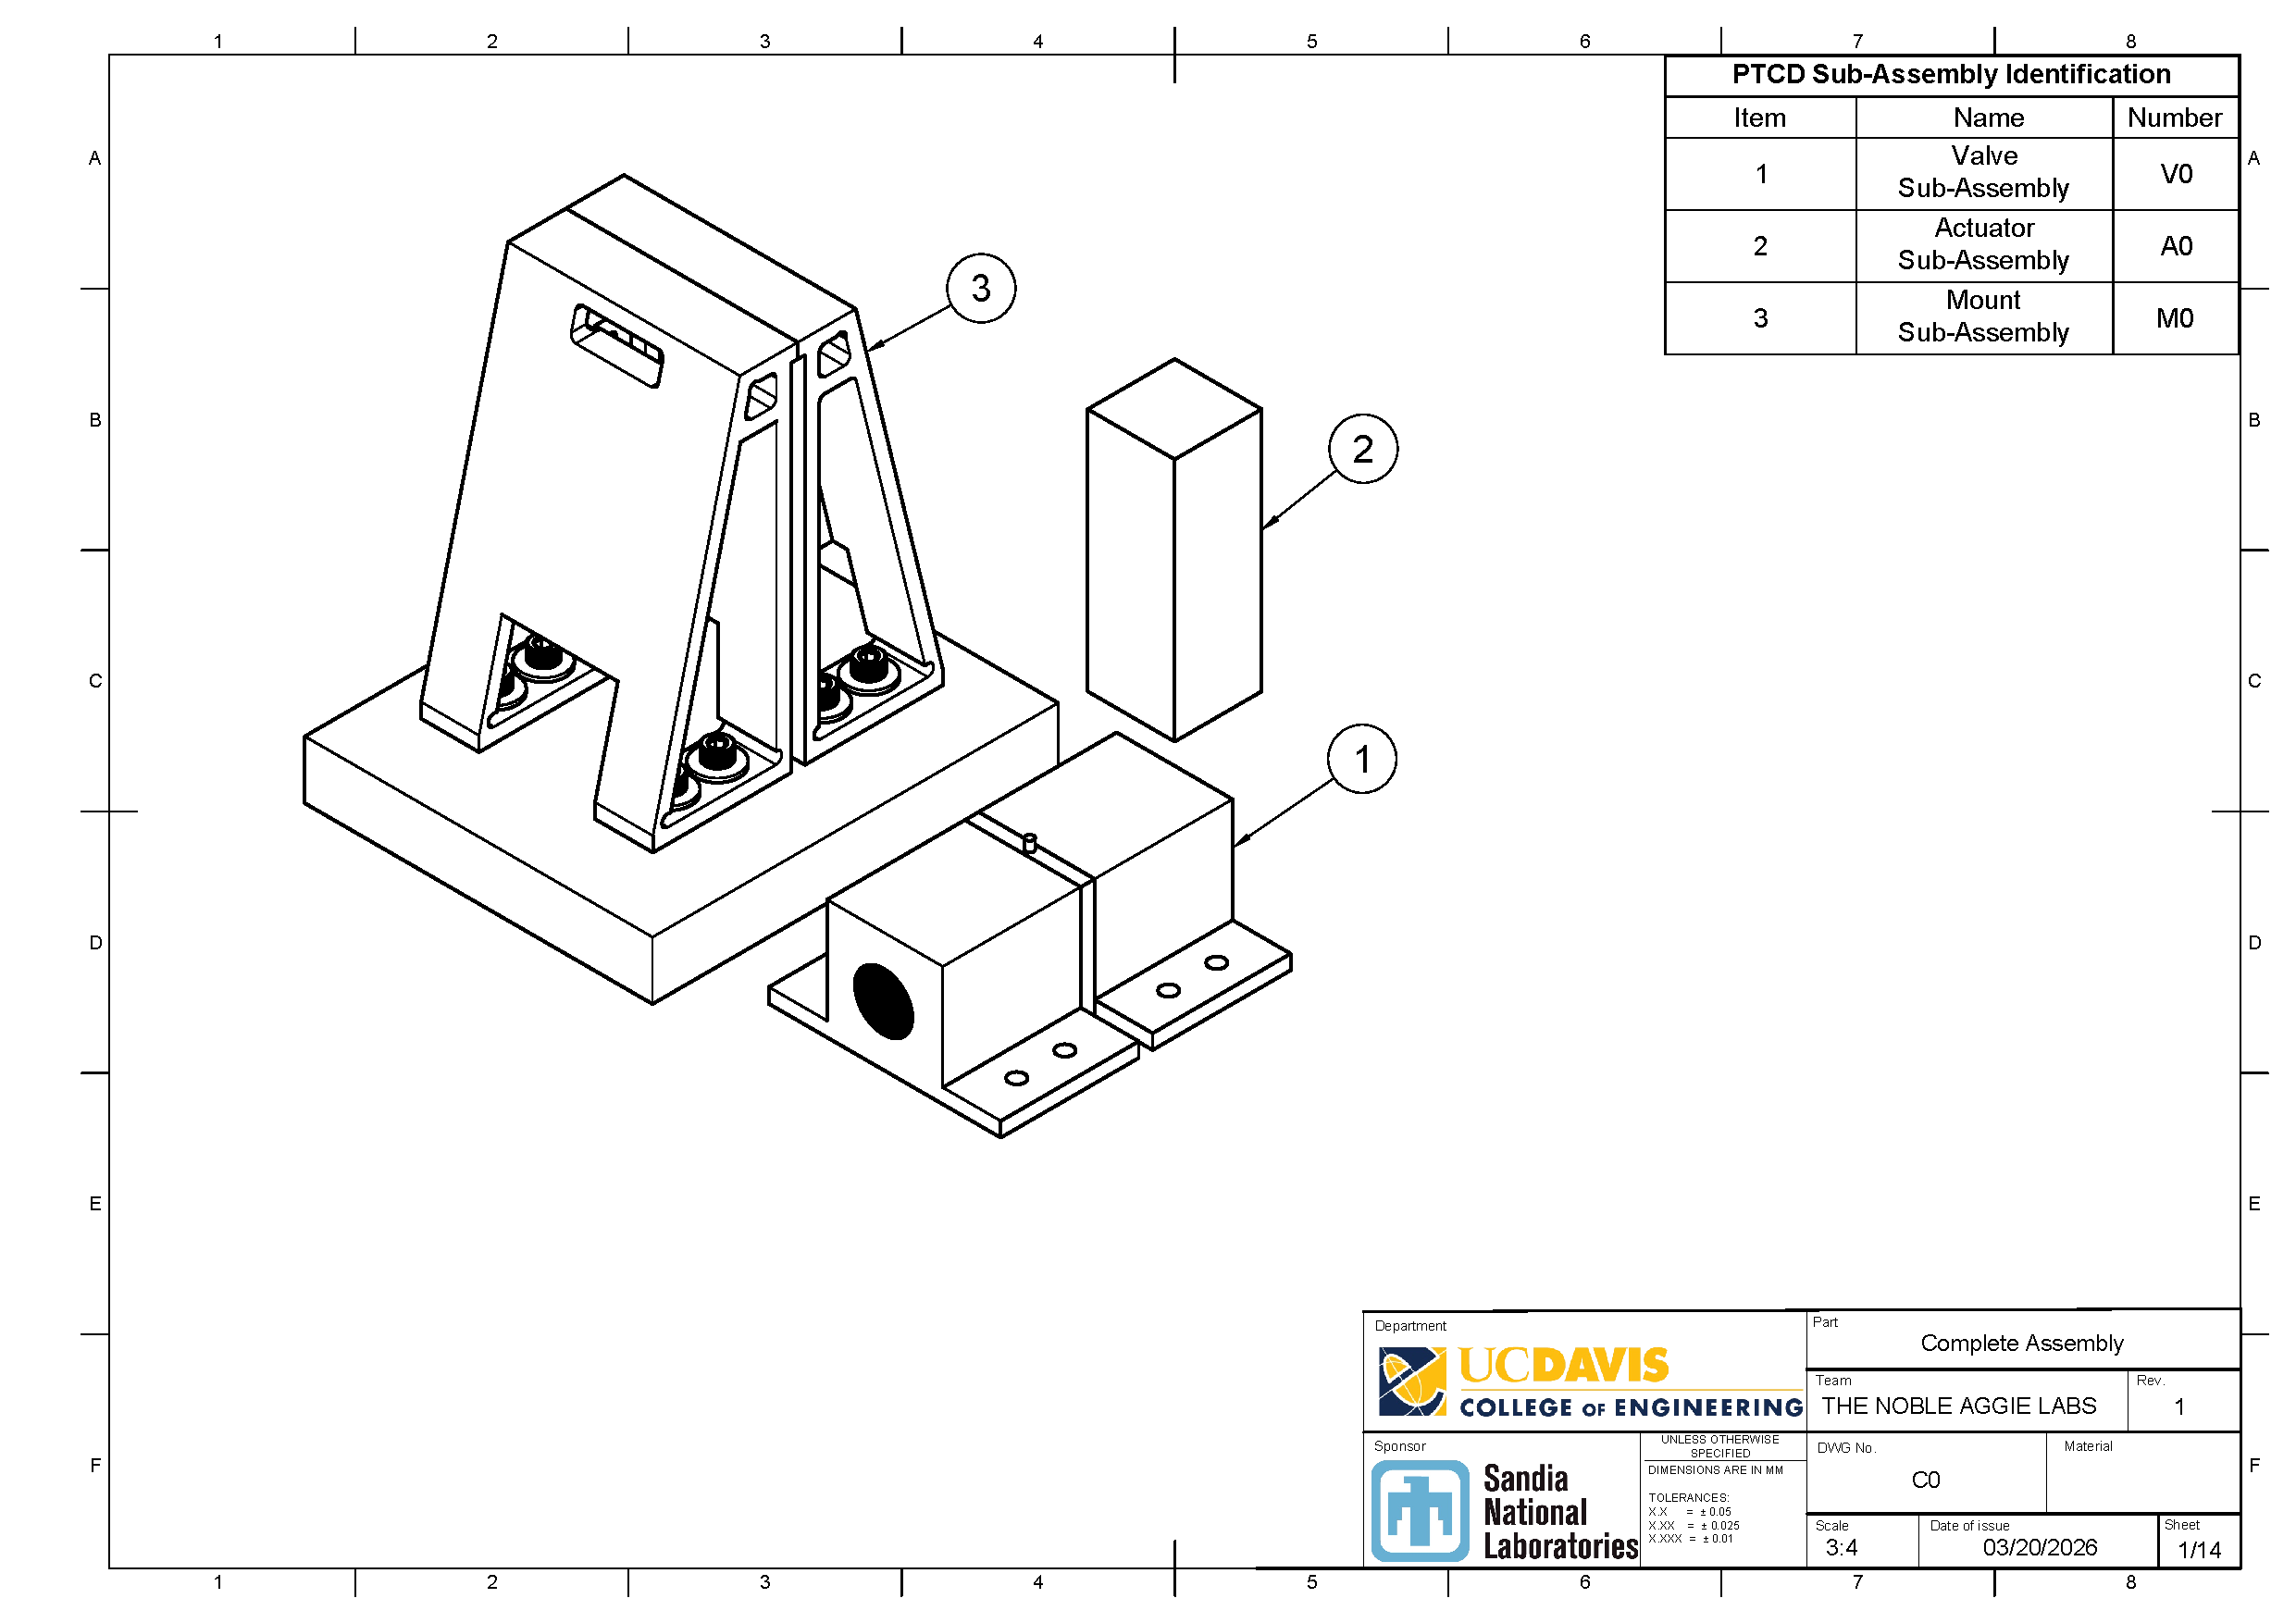
\includepdf[pages=1-14, fitpaper=true, landscape=true]{FinalDrawingPackage.pdf}

% --- Appendix C: Product Data Sheets and Price Quotes ---
\chapter{Bellows Catalog Data Sheet}
\label{app:datasheets}

% The following data sheets are included below:

% \begin{enumerate}
%     \item Mini-Flex bellows (excerpts from their 2026 catalog)
% \end{enumerate}


\includepdf[pages=1-2, fitpaper=true, landscape=true]{bellows_catalog.pdf}


% --- Appendix D: Detailed Calculations ---
\chapter{Detailed Calculations}
\label{app:calculations}

\section{Error Propagation Calculation}
\label{app:errorProp}

    As detailed in Section \ref{sec:initial_system_requirements}, the Required Relationship

        $$ \requiredRelationship $$

    depends on the following independent variables, each with their own tolerance values:

        \begin{align*}
            &A_1 = \specDeffConstOne \specTolerancePercent\ \frac{\text{mm}}\degC
            \\
            &A_0 = \specDeffConstTwo \specTolerancePercent\ \text{mm}
        \end{align*}

    The tolerance of $D_{\text{effective}}$ as a function of temperature can be found using the following formula:

        \begin{equation}
            D_{\text{eff}} = \overline{D_{\text{eff}}}(T) \pm u_D(T)
        \end{equation}

    such that

        \begin{equation}
            u_D(T) = \sqrt{\left( \theta_{A1} \cdot u_{A1} \right)^2 + \left( \theta_{A0} \cdot u_{A0} \right)^2}
            \label{eq:KM_gen}
        \end{equation}

    We can find these values as follows:

        \begin{align}
            &\theta_{A_1}(T) = \frac{\partial D_{\text{eff}}}{\partial A_1} = T - T_{\text{ref}}
            \\
            &u_{A_1} = (5\%)(\SI{-1.52e-6}{m \per \degreeCelsius}) = \SI{-7.62e-8}{} \frac{m}{\degC}
            \\
            &\theta_{A_0} = \frac{\partial D_{\text{eff}}}{\partial A_0} = 1
            \\
            &u_{A_0} = (5\%)(\SI{2.54e-4}{m}) = \SI{1.27e-5}{m}
        \end{align}

    Plugging these into \ref{eq:KM_gen} yields the following tolerance for $D_{\text{effective}}$ as a function of $T_{\text{ambient}}$:

        \begin{equation}
            u_{D_{\text{eff}}} = \sqrt{\left( (\SI{-7.62e-8}{} \frac{m}{\degC}) (T-T_{\text{ref}}) \right)^2 + \left( \SI{1.27e-5}{m} \right)^2}
        \end{equation}

    Therefore, the complete Required Relationship reduces to equations \ref{eq:RR_symb} and \ref{eq:RR_full} in symbolic and numeric form, respectively.

        \begin{align}
            D_{\text{effective}} &= A_1(T_{\text{ambient}}-T_{\text{reference}}) + A_0 \notag \\
                &\quad \pm \sqrt{\left( (0.05)(A_1)(T_{\text{ambient}}-T_{\text{reference}}) \right)^2 + ((0.05)(A_0))^2} \label{eq:RR_symb}
            \\[6pt]
            D_{\text{effective}} &= \SI{-1.52e-6}{} \frac{m}{\degC} (T_{\text{ambient}} - \SI{25}{\degreeCelsius}) + \SI{2.54e-4}{\meter} \notag \\
                &\quad \pm \SI{7.60e-8}{} \frac{m}{\degC} \sqrt{(T_{\text{ambient}} - \SI{25}{\degreeCelsius})^2 + \SI{2.78e4}{\degreeCelsius\squared}} \label{eq:RR_full}
        \end{align}

    Equation \ref{eq:RR_full} can be plotted as a function of temperature with its upper and lower boundaries, as shown in Figure \ref{fig:errorpropboundary}.
    As is evident, the relationship is linear, with the effective diameter decreasing as temperature increases, and the tolerance window is mostly constant.

        \begin{figure}[H]
            \centering
            \begin{tikzpicture}
                \begin{axis}[
                    legend pos=north east,
                    xlabel={$T$},
                    ylabel={$D_{\text{eff}}$},
                ]
                    \addplot[thick, mark=none, color={rgb,255:red,0;green,200;blue,00}] table [x=T, y=D, col sep=comma] {figures/D.csv};
                    \addlegendentry{$\overline{D}(T)$}

                    \addplot[thick, mark=none, red] table [x=T, y=Hi, col sep=comma] {figures/D.csv};
                    \addlegendentry{Upper limit}

                    \addplot[thick, mark=none, blue] table [x=T, y=Lo, col sep=comma] {figures/D.csv};
                    \addlegendentry{Lower limit}
                \end{axis}
            \end{tikzpicture}
            \caption{$D_{\text{eff}}$ with tolerable deviation}
            \label{fig:errorpropboundary}
        \end{figure}

    However, if we plot the tolerance alone, as in Figure \ref{fig:errorpropvariation}, we see that $u_{D_{\text{eff}}}$ varies slightly with temperature.
    Its minimum is at $T_{\text{ref}}$, which motivated the decision to ensure minimum error at this temperature.

        \begin{figure}[H]
            \centering
            \begin{tikzpicture}
                \begin{axis}[
                    xlabel={$T$},
                    ylabel={$u_{D_{\text{eff}}}$},
                ]
                    \addplot[thick, mark=none, blue] table [x=T, y=u_D, col sep=comma] {figures/u_D.csv};

                \end{axis}
            \end{tikzpicture}
            \caption{$u_{D_{\text{eff}}}$ variation with T}
            \label{fig:errorpropvariation}
        \end{figure}

    Finally, the tolerance boundaries for $X(T)$ can be easily found by multiplying every value by $X = \sqrt{\frac{\pi}{2}} D_{\text{eff}}$,
    which relationship is derived in Appendix \ref{app:orifice_geometry}.

        \begin{align}
            X &= \sqrt{\frac{\pi}{2}} \left( A_1(T_{\text{ambient}}-T_{\text{reference}}) + A_0 \right) \notag \\
                &\quad \pm \sqrt{\frac{\pi}{2}} \sqrt{\left( (0.05)(A_1)(T_{\text{ambient}}-T_{\text{reference}}) \right)^2 + ((0.05)(A_0))^2} \label{eq:RR_symb_X}
            \\[6pt]
            X &= \SI{-1.91e-6}{} \frac{m}{\degC} (T_{\text{ambient}} - \SI{25}{\degreeCelsius}) + \SI{3.18e-4}{\meter} \notag \\
                &\quad \pm \SI{9.53e-8}{} \frac{m}{\degC} \sqrt{(T_{\text{ambient}} - \SI{25}{\degreeCelsius})^2 + \SI{2.78e4}{\degreeCelsius\squared}} \label{eq:RR_full_X}
        \end{align}

    As in Figures \ref{fig:errorpropboundary} and \ref{fig:errorpropvariation}, the same can be shown for $X(T)$ in Figures \ref{fig:errorpropboundary_X} and \ref{fig:errorpropvariation_X}.

        \begin{figure}[H]
            \centering
            \begin{tikzpicture}
                \begin{axis}[
                    legend pos=north east,
                    xlabel={$T$},
                    ylabel={$X(T)$},
                ]
                    \addplot[thick, mark=none, color={rgb,255:red,0;green,200;blue,00}] table [x=T, y=X, col sep=comma] {figures/X.csv};
                    \addlegendentry{$\overline{X}(T)$}

                    \addplot[thick, mark=none, red] table [x=T, y=Hi, col sep=comma] {figures/X.csv};
                    \addlegendentry{Upper limit}

                    \addplot[thick, mark=none, blue] table [x=T, y=Lo, col sep=comma] {figures/X.csv};
                    \addlegendentry{Lower limit}
                \end{axis}
            \end{tikzpicture}
            \caption{$X(T)$ with tolerable deviation}
            \label{fig:errorpropboundary_X}
        \end{figure}

        \begin{figure}[H]
            \centering
            \begin{tikzpicture}
                \begin{axis}[
                    xlabel={$T$},
                    ylabel={$u_X$},
                ]
                    \addplot[thick, mark=none, blue] table [x=T, y=u_x, col sep=comma] {figures/u_X.csv};

                \end{axis}
            \end{tikzpicture}
            \caption{$u_X$ variation with T}
            \label{fig:errorpropvariation_X}
        \end{figure}


    This calculation comes from Kline-McClintock error propagation methods used in experimental probability and uncertainty propagation, which states that a dependent variable $x_0 = f(x_1, x_2, x_3...)$,
    such that the tolerance of each independent variable $x_i$ is stated as $\bar{x}_i \pm u_{x_i}$, is represented by its own tolerance value $x_0 = \bar{x}_0 \pm u_{x_0}$ such that
    $$ u_{x_0} = \sqrt{\sum{\left( \theta_{x_i} u_{x_i} \right)^2}} $$
    where $\theta_{x_i} = \frac{\partial x_0}{\partial x_i}\bigg|_{x_i = \overline{x}_i}$ \cite{ref_Figliola}.



\section{Orifice Geometry}
\label{app:orifice_geometry}

    The orifice, as defined in Section \ref{sec:sys_arch_overview} and depicted in Figure \ref{fig: orifice} (shown again in Figure \ref{fig:orifice_rep}), is the "Venn"-style overlap between two angled squares.

    \begin{figure}[H]
        \centering
        
\includegraphics[height=2in]{orifice.png}
        \caption{Orifice geometry, repeated}
        \label{fig:orifice_rep}
    \end{figure}

    \begin{figure}[H]
        \centering
        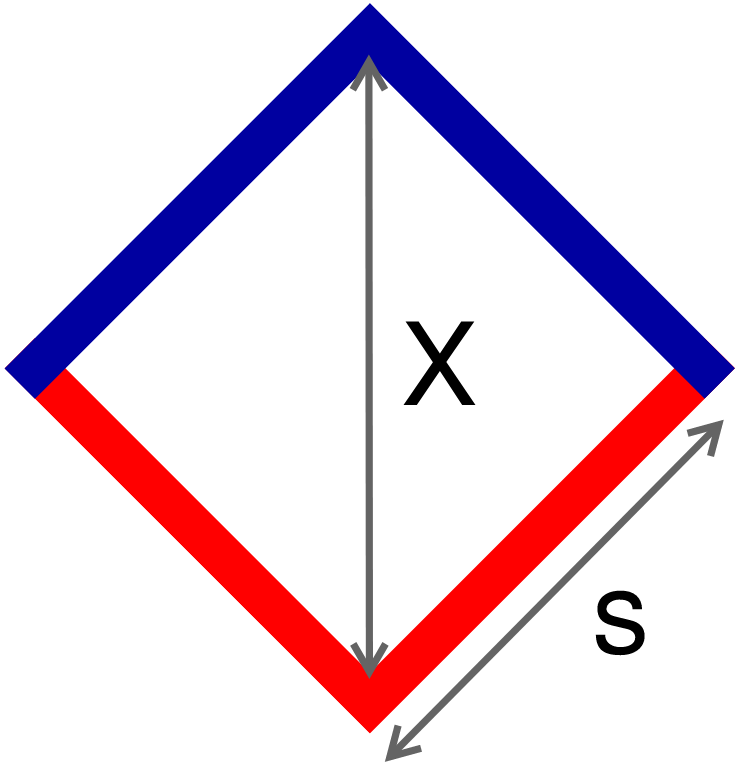
\includegraphics[height=2in]{orifice_detailed.png}
        \caption{Orifice geometry, detailed}
        \label{fig:orifice_detailed}
    \end{figure}

    The effective diameter, as defined in equation \ref{eq:d_eff}, equals the diameter of a circle with equivalent area.
    Thus, the height of the orifice X as defined in Figures \ref{fig: orifice} and \ref{fig:orifice_detailed}, which is directly driven by the actuator movement, 
    can be related to the effective diameter as follows:

        $$ A = \frac{\pi}{4}D_{\text{eff}}^2 = s^2 $$
        $$ s = \sqrt{\frac{\pi}{4}}D_{\text{eff}} $$
        $$ X = \sqrt{s^2 + s^2} = \sqrt{2}s \text{ by the Pythagorean Theorem} $$

    Therefore,

        $$ X = \sqrt{2}\sqrt{\frac{\pi}{4}}D_{\text{eff}} = \sqrt{\frac{\pi}{2}}D_{\text{eff}} $$


\end{appendices}

\end{document}
